\chapter{\scshape KPP surface ocean boundary layer}
\label{chapter:cvmix_kpp}

\minitoc
\vspace{.5cm}

\begin{mdframed}[backgroundcolor=lightgray!50]
  We summarize in this chapter the KPP scheme surface boundary layer
  scheme \citep{LargeKPP} as implemented in CVMix.  CVMix provides the
  same features as that suggested by \cite{LargeKPP} and Appendix A of
  \cite{Dana_etal2006}.  However, for those not intent on recovering
  older results, we recommend simplifying the non-dimensional shape or
  structure function $G(\sigma)$, with this recommendation based on
  testing conducted during the CVMix implementation.  The following
  CVMix Fortran module is directly connected to the material in this
  chapter:
\begin{align*} 
 & {\tt cvmix\_kpp.F90}
\end{align*}
\end{mdframed}


\section{Elements of the K-profile parameterization (KPP)}
\label{sec:implementation}

The ocean surface boundary layer (OBL) mediates the exchange of
properties between the ocean and other components of the climate
system. Hence, parameterization of processes active in the OBL are
fundamental to the integrity of a climate simulation. The K-profile
parameterization (KPP) is a widely used method for parameterizing
boundary layer processes in both the atmosphere and ocean.\footnote{We
  consider here the implementation of KPP for the surface ocean
  boundary layer, as implementations for the bottom do not exist in
  MOM or POP.  \citep{Durski_etal2004} consider KPP for the ocean
  bottom in ROMS.} The paper by \cite{LargeKPP} introduced this scheme
to the ocean community for use in parameterizing processes in the
surface ocean boundary layer .  The pedagogical lectures by
\cite{LargeKPP_lectures} and \cite{Large2012} provide added insight
into the scheme that complements some of the material in
\cite{LargeKPP}.

The KPP scheme has been used by many ocean climate studies for
parameterizing mixing in the OBL, with examples discussed in
\cite{Largeforcing}, \cite{HollandChowBryan1998},
\cite{Gent_etal_1998}, \cite{GOTM}, \cite{LiChowMcWilliamsFu2001},
\cite{Smyth_etal2002}, \cite{Durski_etal2004}, and
\cite{Chang_etal2005}).  It was also used in various climate and earth
system models developed at NCAR and GFDL, and elsewhere.  

We aim to be thorough in exposing the physical aspects of the KPP
scheme, building on the previous discussions in \cite{LargeKPP} and
\cite{Large2012}.  We also discuss certain of the issues that arose
when testing the scheme for use in CVMix that further motivate the
choices and provide suggestions for how to make use of the CVMix
version of KPP for ocean modeling purposes. Correspondingly, we
motivate simplifications to the scheme available in CVMix, relative to
the original implementation based on \cite{LargeKPP}.


\subsection{Conventions}
\label{subsection:conventions}

We use the following notational and sign conventions in this chapter. 

\begin{itemize}
 
\item The fluid is assumed to be volume conserving Boussinesq, with
  extensions to a mass conserving non-Boussinesq fluid trivial.

\item \label{geopotential_defined} The geopotential coordinate, $z$,
  which increases up and where $z=0$ defines the resting ocean
  surface. The ocean free surface is defined by $z=\eta(x,y,t)$ and
  the static ocean bottom is at $z=-H(x,y)$.

\item \label{lambda_defined} A lowercase $\lambda$ is used to denote a
  turbulent fluctuation of an arbitrary field within the surface ocean
  boundary layer; e.g., a tracer such as potential or conservative
  temperature $\theta$ and salinity $s$), or a velocity component
  ($u,v,w$). Note that $x$ is the notation used in \cite{LargeKPP} and
  \cite{LargeKPP_lectures}, but we prefer the Greek letter $\lambda$
  to avoid confusion with the horizontal spatial coordinate.  Also,
  the symbol $s$ is somtimes used for scalar fields such as salinity
  and temperature, whereas $m$ is sometimes used for components of a
  vector field.  

\item There is no distinction in the treatment of scalar fields within
  the KPP boundary layer.  It is only beneath the boundary layer,
  where double diffusive processes are relevant, that we distinguish
  the mixing between scalar fields such as temperature and salinity.
  Also, the surface forcing for salt/scalars and heat distinguishing
  the tracers.

\item \label{Lambda_defined} An uppercase $\Lambda$ is used to denote
  the Eulerian mean of a tracer or velocity component within the
  surface ocean boundary layer; e.g., potential or conservative
  temperature $\Theta$, salinity $S$, or velocity component ($U,V,W$).
  The Eulerian mean fields are time stepped by an ocean climate model
  within the boundary layer, and correlations of turbulent variables
  must be parameterized to close the mean field equations.

\item \label{correlation_defined} The expression $\overline{w \,
    \lambda}$ is used to symbolize the Eulerian correlation of the
  fluctuating turbulent vertical velocity and a fluctuating scalar or
  vector field. This correlation appears in the mean field time
  tendency equation for $\Lambda$ in the Boussinesq primitive ocean
  equations (see equation (\ref{eq:mean-field-equation-kpp})). KPP
  provides a parameterization of this vertical turbulent flux within
  the surface ocean boundary layer.

\item \label{w_W_defined} The mean and turbulent vertical velocity
  components, $W,w$, are positive for upward motion. This sign
  convention implies that
\begin{mdframed}[backgroundcolor=lightgray!50]
   \begin{equation}
  \overline{w \, \lambda}  > 0  \implies \mbox{turbulent flux for $\lambda$ transported vertically upward}.
\label{eq:correlation-convention}
\end{equation}
\end{mdframed}
If $\lambda$ is the temperature, then a positive correlation at the
ocean surface, 
\begin{equation}
 \overline{w \, \theta}^{d=0} > 0,
\end{equation}
corresponds to surface cooling.  To reduce notation clutter,
correlations evaluated at the ocean surface will be written
\begin{equation}
 \overline{w \, \theta}^{0} =  \overline{w \, \theta}^{d=0}.
\end{equation}

\item Boundary fluxes of scalar fields are denoted by a capital $Q$,
  along with a subscript or superscript to denote the particular flux.
  Such scalar fluxes are assumed to be positive when entering the
  ocean and negative when leaving the ocean
\begin{mdframed}[backgroundcolor=lightgray!50]
\begin{equation}
  Q > 0 \Rightarrow \mbox{boundary scalar flux enters the ocean.} 
\label{eq:boundary-sign-convention}
\end{equation}
\end{mdframed}


\item We make the following observations about the sign conventions
  (\ref{eq:correlation-convention}) and
  (\ref{eq:boundary-sign-convention}).
\begin{itemize}
\item A positive heat flux, $Q^{\mbox{\footnotesize heat}} > 0$,
  either through the ocean surface or ocean bottom, adds heat to the
  ocean; likewise for salt and water.

\item The sign convention (\ref{eq:boundary-sign-convention}) is
  followed in MOM and POP.  However, it is not the convention used in
  \cite{LargeKPP}, whose convention was in fact opposite for some
  cases except for penetrative radiation.

\item We consider a positive surface buoyancy forcing, $B_{f} > 0$
  (units $\mbox{m}^{2}~\mbox{s}^{-3}$), to increase the ocean
  buoyancy.  Adding heat to the ocean increases its buoyancy in
  regions of positive thermal expansion, whereas adding salt decreases
  buoyancy in regions of positive haline contraction.

\item The convention (\ref{eq:boundary-sign-convention}) necessitates
  a minus sign when equating surface boundary fluxes of scalars to the
  correlations $\overline{w \, \lambda}^{0}$ defined by equation
  (\ref{eq:correlation-convention}).

\item At the ocean bottom, the convention requires no minus sign,
  since $\overline{w \, \lambda}^{-H} > 0$ means there is a transfer
  of scalar field into the ocean through the ocean bottom, such as
  through geothermal heating.  Note that we are not concerned with
  implementing KPP at the ocean bottom \citep{Durski_etal2004}.

\end{itemize}

\item Momentum imparted to the ocean surface by a boundary stress,
  $\bftau$, acts to accelerate the ocean in the respective direction.
  In contrast, a positive sign to a component of $\overline{w \, {\bf
      u}}^{0}$ removes the associated momentum from the surface
  ocean.  These sign conventions give rise to the minus sign in the
  relation (\ref{eq:wu-kinematic-flux-kpp}) connecting turbulent
  kinematic stress to the boundary stress: $-\rho \, \overline{w \,
    {\bf u}}^{0} = \bftau$.  

\end{itemize}

 
\subsection{General form of the KPP parameterization}

Ignoring all terms except vertical advective transport in the
prognostic equation for the mean field $\Lambda$, its time tendency 
is determined by 
\begin{equation}
 \frac{\partial \Lambda}{\partial t} = -\left( \frac{\partial \, (W \, \Lambda)}{\partial z} \right)  
 -\left( \frac{\partial \, (\overline{w \, \lambda}) }{\partial z} \right).  
\label{eq:mean-field-equation-kpp}
\end{equation}
The advective flux by the mean vertical velocity, $W \, \Lambda$, is
represented via a numerical advection operator. In contrast, the
turbulent correlation, $\overline{w \, \lambda}$, is a subgrid scale
flux that must be parameterized in order to close the equation for
$\Lambda$. Here, the overbar signifies an Eulerian averaging operator
over unresolved turbulent motions occurring within the OBL.

The KPP scheme provides a first order closure for $\overline{w \,
  \lambda}$ within the OBL. It does so by introducing two terms in the
following manner 
\begin{equation}
  \overline{w \, \lambda} = -K_{\lambda} \left( \frac{\partial \Lambda}{\partial z}  \right)
   +  K^{\mbox{\tiny non-local}}_{\lambda}  \, \gamma_{\lambda}.
\label{eq:kpp-parameterization}
\end{equation}
The KPP prescription (\ref{eq:kpp-parameterization}) thus
parameterizes the vertical turbulent flux using two terms
\begin{equation}
  \overline{w \, \lambda} = \overline{w \, \lambda}^{\mbox{\tiny local}} + \overline{w \, \lambda}^{\mbox{\tiny non-local}}.
\label{eq:vertical-flux-decomposed}
\end{equation}
The first term provides for the familiar downgradient vertical
diffusion determined by a vertical diffusivity and the local vertical
derivative of the mean field.  This term is referred to as the local
portion of the parameterization
\begin{equation}
\overline{w \, \lambda}^{\mbox{\tiny local}} = -K_{\lambda}  \left( \frac{\partial \Lambda}{\partial z} \right).
\label{eq:vertical-flux-local}
\end{equation}
Note that the diffusivity $K_{\lambda} $ computed from KPP is a
non-local function of boundary layer properties, so the name ``local''
is not directed at the diffusivity, but instead at the vertical
derivative.  The second term, $\gamma_{\lambda}$, accounts for
non-local transport that is not directly associated with local
vertical gradients of $\Lambda$, in which
\begin{equation}
  \overline{w \, \lambda}^{\mbox{\tiny non-local}} = K^{\mbox{\tiny non-local}}_{\lambda} \; \gamma_{\lambda}.
\label{eq:vertical-flux-nonlocal}
\end{equation}


\subsection{The vertical diffusivity}
\label{subsection:kpp-vertical-diffusivity}

The vertical diffusivity used to parameterize the local flux
(\ref{eq:vertical-flux-local}) arising from KPP in the OBL is
determined as a non-local function of boundary layer properties. It is
written in the following form
\begin{equation}
  K_{\lambda}(\sigma) = h \, w_{\lambda}(\sigma) \, G_{\lambda}(\sigma).
\label{eq:kpp-diffusivity}
\end{equation}
The diffusivity is a constructed as the product of three terms: the
boundary layer thickness $h$, the vertical turbulent velocity scale
$w_{\lambda}(\sigma)$, and the vertical shape or structure function
$G_{\lambda}(\sigma)$.  Note that we introduce a dependence of the
shape function on the field diffused.  Such dependence can arise if
taking the approach of \cite{LargeKPP} whereby the boundary layer
diffusivity is matched at the base of the boundary layer to the
interior diffusivities, which can generally be a function of the
tracer, $\lambda$.  However, as discussed in Section
\ref{subsection:kpp-shape-function-cvmix}, the recommended approach
for CVMix is to use the following universal shape function for all
tracers (equation (\ref{eq:universal-non-local-structure}))
\begin{equation}
 G(\sigma)_{\mbox{\tiny universal}} = \sigma \, \ (1-\sigma)^{2},
\label{eq:simpler-shape-function-first}
\end{equation}
 thus greatly simplifying the KPP scheme. 

\cite{LargeKPP} proposed to set the diffusivities equal
\begin{equation}
 K^{\mbox{\tiny non-local}}_{\lambda} = K_{\lambda},
\end{equation}
and we support that recommendation, along with setting the shape
function to the universal form
(\ref{eq:simpler-shape-function-first}).  However, in moving from the
\cite{LargeKPP} version of KPP to this simplified version, one may
choose to test an intermediate version in which the non-dimensional
shape function is distinct for $K^{\mbox{\tiny non-local}}_{\lambda}$
and $K_{\lambda}$.  It is for this reason that we maintain the
distinct symbols for the diffusivities, even though we recommend users
choose the CVMix implementation of KPP that sets them equal.  We have
more to say on this topic in Section
\ref{subsection:kpp-shape-function}.


\subsubsection{Boundary layer thickness} 

The boundary layer thickness is denoted by 
\begin{equation}
 h \ge 0 \; \; \mbox{is the boundary layer thickness}.
\label{eq:boundary-layer-thickness}
\end{equation}
This is the thickness of the OBL prescribed by the KPP scheme, with
details given in Section \ref{subsection:kpp-obl-thickness}.  The
surface boundary layer generally thickens when mechanical forcing
mixes the water, and negative buoyancy forcing makes the water
gravitationally unstable.  Conversely, the bounday layer shoals with
weak winds and/or positive buoyancy forcing.  The direct dependence of
the vertical diffusivity in equation (\ref{eq:kpp-diffusivity}) on the
OBL thickness manifests the common property of boundary layers,
whereby thicker layers generally arise from stronger eddy motions and
are thus associated with more rapid mixing of tracer concentration and
momentum.

Figure \ref{fig:boundary-layer-schematic-kpp} provides a schematic of
the KPP boundary layer, the Monin-Obukhov surface layer, and the
associated momentum, mass, and buoyancy fluxes impacting these layers.
Details of this figure will be explored in the following.



\subsubsection{Measuring vertical distances within the OBL}

When measuring distances within the boundary layer, it is the
thickness of the water as measured from the ocean surface that is
important. Free surface undulations can be a nontrivial fraction of
the boundary layer thickness, particularly under conditions of stable
buoyancy forcing. Hence, we make explicit note that the ocean has an
undulating free surface at $z=\eta(x,y,t)$, which contrasts to
\cite{LargeKPP} and \cite{LargeKPP_lectures}, who assumed that $z=0$
sets the upper ocean surface.

Following \cite{LargeKPP}, we introduce the non-dimensional depth,
$\sigma$, given by 
\begin{equation}
  \sigma = \frac{d}{h}.
\label{eq:sigma-defined}
\end{equation}
In this definition, $d \ge 0$ is the distance from the ocean surface
at $z=\eta$ to a point within the boundary layer
\begin{equation}
  d = -z+\eta.
\label{eq:distance-from-surface-defined}
\end{equation}
Likewise, $h \ge 0$ is the distance from the free surface 
to the bottom of the boundary layer
\begin{equation}
  h = h_{\mbox{\tiny obl}} +\eta,
\label{eq:h-obl-defined}
\end{equation}
where $h_{\mbox{\tiny obl}}$ is the depth of the boundary layer as
measured from $z=0$. That is, $h$ is the thickness of the OBL, and it is this 
thickness, not $h_{\mbox{\tiny obl}}$, that is
predicted  by KPP (Section \ref{subsection:kpp-obl-thickness}).
Regions within the boundary layer are given by the non-dimensional
depth range
\begin{equation}
  0 \le \sigma \le 1 \qquad \mbox{within boundary layer,}
\end{equation}
with $\sigma=0$ the ocean surface and $\sigma = 1$ the bottom of the
boundary layer.



%%%%%%%%%%%%%%%%%%%% %%%%%%%%%%%%%%%%%%%%%%%%%
\begin{figure}[h!t]
\rule{\textwidth}{0.005in}
\begin{center}
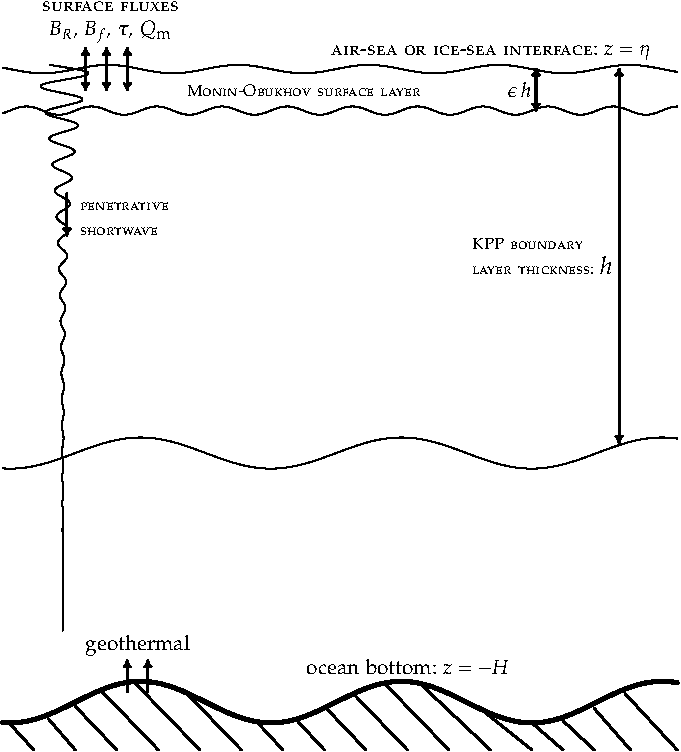
\includegraphics[angle=0,width=10cm]{./mfpic_figs/cvmix_kpp_boundary_layer.pdf}
\caption[KPP boundary layer schematic]{\sf Schematic of the upper
  ocean boundary layer regions associated with the KPP boundary layer
  parameterization.  The upper ocean is exposed to non-penetrative
  air-sea and ice-sea fluxes of momentum $\bftau$ (Section
  \ref{section:boundary-forcing-momentum-kpp}), mass $\Qm$(Section
  \ref{section:boundary-forcing-buoyancy-kpp}), and buoyancy $B_{f}$
  (Section \ref{section:boundary-forcing-buoyancy-kpp}).  In addition,
  there is penetrative shortwave radiation, $-\overline{w \,
    \theta}_{R}$ (Section
  \ref{section:boundary-forcing-buoyancy-kpp}), indicated by the
  exponentially decaying vertical sinusoidal.  The Monin-Obukhov
  surface layer (Section \ref{section:m-o-similarity}) has a thickness
  $\epsilon \, h$, with $\epsilon \approx 0.1$.  The surface layer is
  where turbulence delivers fluxes to the molecular skin layer for
  transfer to the atmosphere or ice.  The surface layer starts from
  just beneath the surface roughness elements at the upper ocean
  interface.  Since neither these roughness elements, nor the
  molecular viscous sublayer, are resolved in ocean models, we assume
  in practice that the Monin-Obukhov surface layer extends to the sea
  surface at $z=\eta(x,y,t)$.  The KPP boundary layer includes the
  surface layer, and it has a thickness $h(x,y,t)$ determined by the
  KPP parameterization (Section \ref{subsection:kpp-obl-thickness}).
  The ocean bottom at $z=-H(x,y)$ is rigid and is exposed to
  geothermal heating.  Presently, the KPP boundary layer scheme has
  not been implemented in MOM or POP to parameterize bottom boundary
  layer physics, though nothing fundamental precludes such.  In fact,
  \cite{Durski_etal2004} provide just such an implementation.}
\label{fig:boundary-layer-schematic-kpp}
\end{center}
\rule{\textwidth}{0.005in}
\end{figure}
%%%%%%%%%%%%%%%%%%%%%%%%%%%%%%%%%%%%%%%%%%%%%%%%%%%%%%%%%%%%%%%%%%%%%%%%


\subsubsection{Scale for turbulent vertical velocity fluctuations $w_{\lambda}$}
\label{subsubsection:turbulent-vertical-velocity-scale}

We introduce a scale for turbulent vertical velocity fluctuations,
written as $w_{\lambda}(\sigma)$.  It is a function of depth within
the boundary layer, and a function of the field to which it refers.
\cite{LargeKPP} recommend using the {\it same} scale $w_{s}$ for all
scalar fields (temperature, salinity, and passive tracers)
\begin{equation}
  w_{s}= \mbox{same for all scalars}.
\end{equation}
The scale $w_{s}$ also is the same as the turbulent velocity scale for
momentum, $w_{m}$, in cases where the surface buoyancy forcing,
$B_{f}$ is positive.  However, $w_{m} < w_{s}$ under unstable surface
buoyancy forcing
\begin{subequations}
\begin{align}
  w_{m}  &= w_{s}  \qquad B_{f} > 0 \\
   w_{m} &< w_{s} \qquad B_{f} < 0.
\end{align}
\end{subequations}
That is, gravitational instability is assumed to mix scalars more
efficiently than momentum.  We return to the specification of
$w_{\lambda}$ in Section \ref{subsection:vertical-velocity-scale}.


\subsubsection{Non-dimensional vertical shape function $G_{\lambda}(\sigma)$}

Non-dimensional vertical shape function $G_{\lambda}(\sigma)$ is used to
smoothly transition from the ocean surface to the bottom of the
boundary layer. \cite{LargeKPP} chose a cubic polynomial
\begin{equation}
 G_{\lambda}(\sigma) = a_{0} + a_{1} \, \sigma + a_{2} \, \sigma^{2} + a_{3} \, \sigma^{3}.
\label{eq:shape-function-gsigma}
\end{equation}
Since turbulent eddies do not cross the ocean surface at $\sigma=0$,
we should correspondingly have a vanishing diffusivity at $\sigma=0$.
This constraint is satisfied by setting 
\begin{equation}
 a_{0} = 0.
\end{equation}
We detail in Section \ref{subsection:kpp-shape-function} how to
specify the remaining expansion coefficients $a_{1}, a_{2}, a_{3}$
following the approach from \cite{LargeKPP}, in which the polynomial
coefficients $a_{1}, a_{2}, a_{3}$ depend on the tracer fields in so
far as they are specified by matching to the interior diffusivities.
Double diffusive processes lead to distinct diffusivities for
temperature and material tracers such as salt.  

However, as discussed in Section \ref{subsection:kpp-shape-function},
the recommended approach for CVMix is to use the following universal
shape function for all tracers (equation
(\ref{eq:universal-non-local-structure}))
\begin{equation}
 G(\sigma)_{\mbox{\tiny universal}} = \sigma \, \ (1-\sigma)^{2},
\end{equation}
thus greatly simplifying the KPP scheme. With this universal shape
function, we have
\begin{equation}
 G(0)_{\mbox{\tiny universal}}= G(1)_{\mbox{\tiny universal}} = G'(1)_{\mbox{\tiny universal}} = 0,
\end{equation}
which is the form suggested by atmospheric boundary layer
implementations of KPP (see Figure \ref{fig:kpp-figure2-reproduced}).


\subsection{The non-local transport $\gamma_{\lambda}$}
\label{subsection:kpp-nonlocal-transport-outline}

There are many processes in the boundary layer that lead to transport
that is difficult to parameterize as a function of the local vertical
derivative of the mean field (see Section 2 of \cite{LargeKPP}).  This
behaviour leads to a diffusivity $K_{\lambda}$ that is a function of
the surface fluxes and boundary layer thickness $h$.  Furthermore,
under convective forcing (negative surface buoyancy forcing; $B_{f} <
0$), fluxes can penetrate into stratified interior.  This
characteristic then motivates the introduction of a non-local
transport term $\gamma_{\lambda}$ to the KPP parameterization
(equation (\ref{eq:kpp-parameterization})) in the case of $B_{f} < 0$.
To further identify the need for a non-local transport term
$\gamma_{\lambda}$, we reproduce Figure 1 from \cite{LargeKPP}, here
shown as Figure \ref{fig:kpp-figure1-reproduced}.  The caption to
Figure \ref{fig:kpp-figure1-reproduced} explores the many facets of
this figure used to help justify the non-local term in KPP.

%%%%%%%%%%%%%%%%%%%% %%%%%%%%%%%%%%%%%%%%%%%%%
\begin{figure}[h!t]
\rule{\textwidth}{0.005in}
\begin{center}
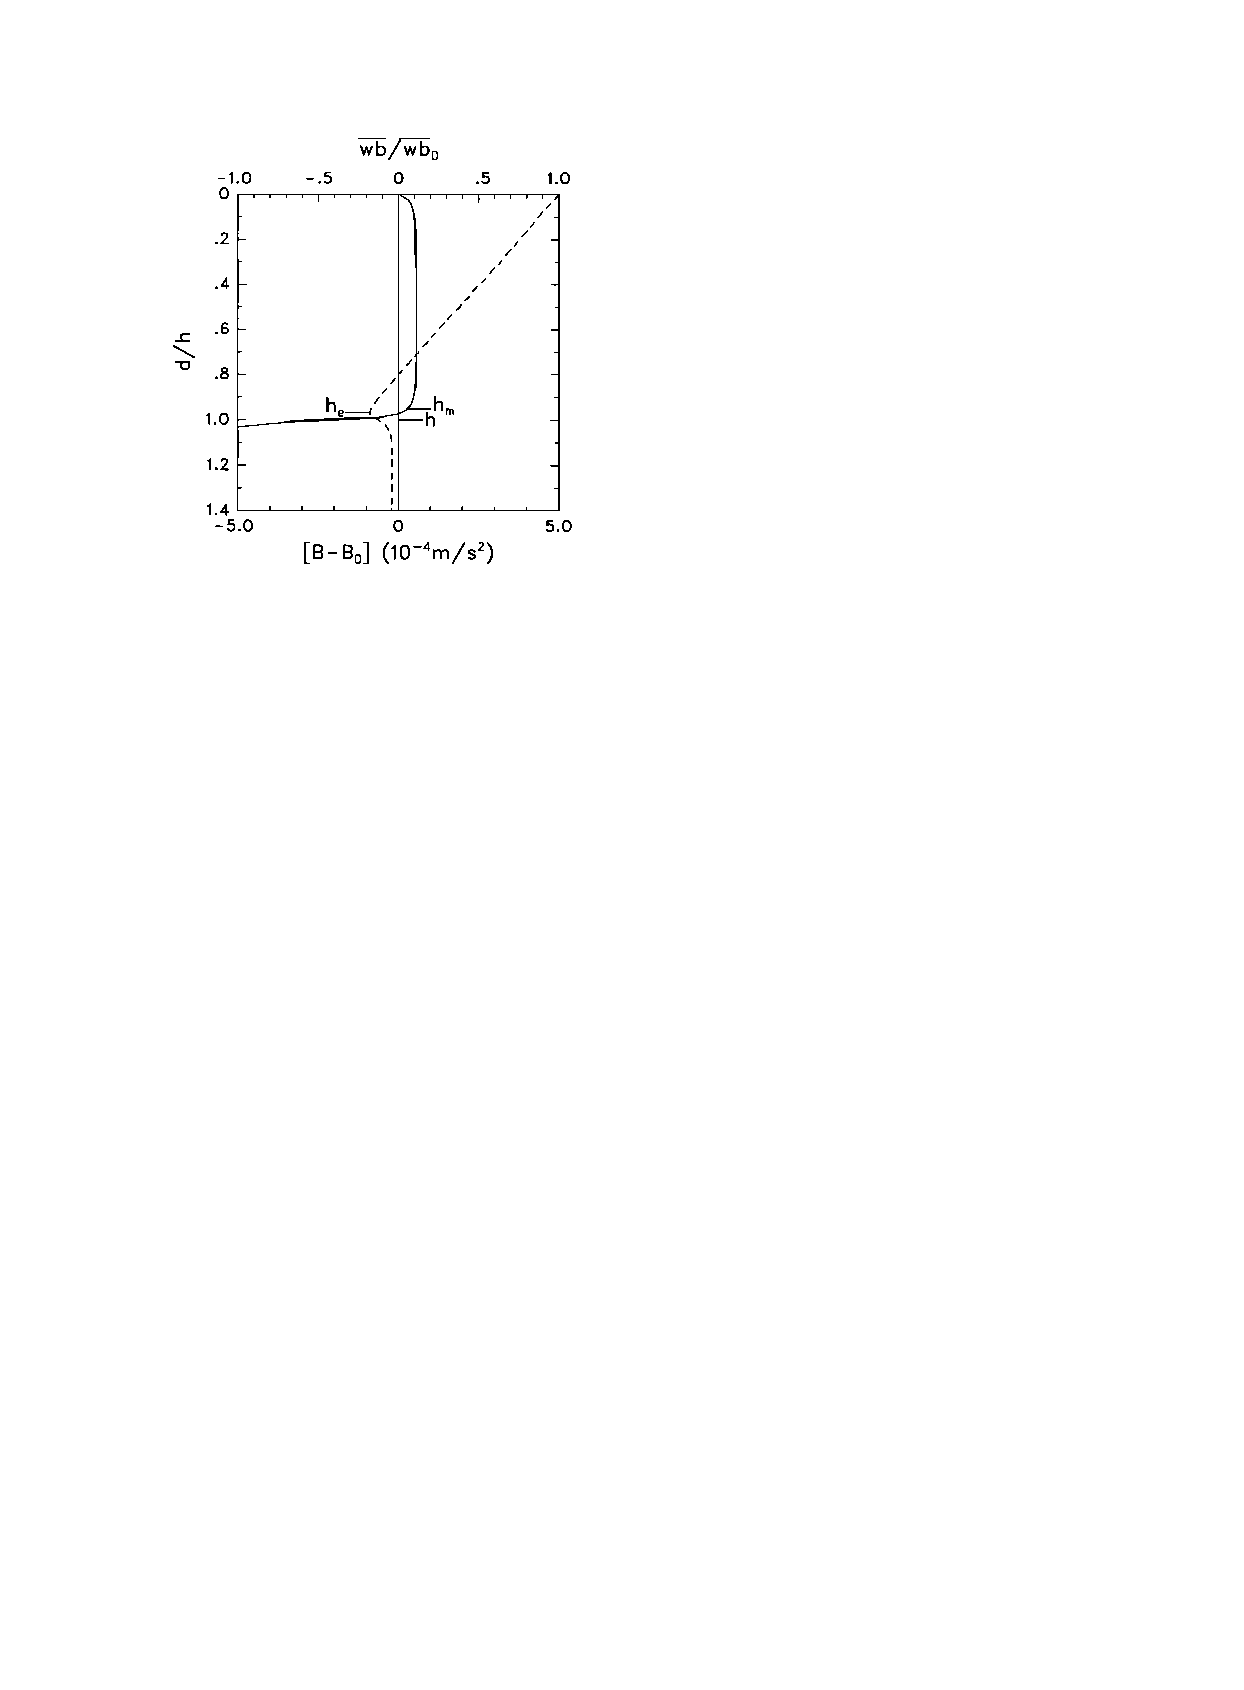
\includegraphics[angle=0,width=10cm]{./figs/LargeKPP_fig1.pdf}
\caption[Figure 1 from \cite{LargeKPP}]{
  \sf
This is a reproduction of
  Figure 1 from \cite{LargeKPP}.
  The figure is derived from a one-dimensional simulation after 3 days of
  convective deepening (zero winds; negative surface buoyancy forcing)
  into an initially uniformly  stratified water column.  The vertical axis
  is vertical distance starting from the ocean surface interface at
  $z=\eta$ and $d=0$, extending down to $d=h$ ($h=13.6$~m at this point
  of the integration), which is the base of
  the boundary layer, and finally to $d=1.4\, h$, which is beneath the
  boundary layer.

 \hspace{0.4cm} The horizontal axis on the bottom is the mean buoyancy, $B$,
  relative to that at the surface, $B_{0}$, and the profile is
  depicted by the solid line. Positive values of
  $B-B_{0}$ indicate that the mean buoyancy at a point is larger than 
  at the surface, with $B-B_{0} > 0$ expected under
  negative buoyancy forcing at the ocean surface.  

  \hspace{0.4cm}  The horizontal axis on
  the top is the ratio of the local turbulent buoyancy flux
  $\overline{w \, b}$ to the surface turbulent flux $\overline{w \,
    b}^{0}$ (denoted $\overline{w \, b}_{0}$ by \cite{LargeKPP}).
  The dashed line depicts this ratio.  Positive values of $\overline{w
    \, b}$ represent upward turbulent buoyancy fluxes; e.g., upward
  fluxes of heat (ocean surface cooling)  for the case where buoyancy is determined by
  temperature, and the thermal expansion coefficient is positive.
  
  \hspace{0.4cm}  Positive values for $\overline{w \, b}$  in regions between roughly $0.35 < d
  < 0.8$ represent upward turbulent buoyancy fluxes in a region where the mean vertical
  gradient of $B$ is nearly zero, thus indicating non-local turbulent transport.
  In shallower regions with $d < 0.35$, the mean gradient is negative,
  $\partial_{z} B < 0$, and the fluxes are positive, $\overline{w \,
    b} > 0$, thus representing downgradient turbulent fluxes.
  Likewise, for $d> 0.8$, the turbulent fluxes are downgradient.

  \hspace{0.4cm} The mixed layer depth is denoted by $h_{m}$, though
  this depth is subject to arbitrary specification of the density
  difference. The entrainment depth is $h_{e}$, with this depth taken
  where the buoyancy flux reaches a negative extrema. Note that it is
  an empirical result that under pure convective forcing ($\bftau =0,
  B_{f} < 0$), the turbulent entrainment flux is roughly 20\% of the
  surface flux: $\overline{w \, b}^{d=h_{e}} = \beta_{T} \;
  \overline{w \, b}^{0}$, where $\beta_{T} = -0.2$. This situation is
  depicted in the figure. }
\label{fig:kpp-figure1-reproduced}
\end{center}
\rule{\textwidth}{0.005in}
\end{figure}
%%%%%%%%%%%%%%%%%%%%%%%%%%%%%%%%%%%%%%%%%%%%%%%%%%%%%%%%%%%%%%%%%%%%%%%%


As part of the KPP parameterization, the non-local transport,
$\gamma_{\lambda}$, aims to account for such processes as boundary
layer eddies whose transport may be unrelated to the local vertical
gradient of the mean field, and whose impacts may penetrate within the
stratified ocean interior. In general, \cite{LargeKPP} prescribe the
following characteristics to $\gamma_{\lambda}$.
\begin{itemize}

\item Page 371 of \citep{LargeKPP} notes that there is no theory for
  non-local momentum transport, so the non-local transport is assumed
  to directly affects only the tracer fields:
\begin{equation}
 \gamma_{\lambda} \; \; = \; \; 
\left\{
 \begin{array}{ll}
  0 \; \;  &\mbox{if $\lambda = (u,v,w)$ a velocity component}
 \\
  \ne 0 \; \; &\mbox{nonzero if $\lambda = \theta,s$ or another tracer.}
  \end{array}
 \right.
\end{equation}
\cite{Smyth_etal2002} consider a non-local term for momentum, thus
motivating further research to see whether it is suitable for climate
modeling.  CVMix has not implemented the \cite{Smyth_etal2002} scheme.
However, CVMix has hooks available in the code for a non-local
momentum transport term, thus facilitating further development of
their ideas.

  \item The non-local transport is non-zero only within the OBL:  
\begin{equation}
 \gamma_{\lambda} \; \; = \; \; 
  \left\{ 
  \begin{array}{ll}
   0 \; \; &\mbox{if $\sigma > 1$}
   \\ 
   \ne 0  \; \; &\mbox{if $0 \le \sigma \le 1$.}
  \end{array}
 \right.
\end{equation}

  \item The non-local transport is non-zero only in the presence of
    destabilizing negative surface ocean buoyancy flux, whose presence
    gives rise to convective mixing:
\begin{equation}
 \gamma_{\lambda} \; \; = \; \; 
  \left\{ 
  \begin{array}{ll}
   0 \; \; &\mbox{for positive (stabilizing) surface buoyancy forcing}
   \\ 
   \ne 0  \; \; &\mbox{for negative (destabilizing) surface buoyancy forcing.}
  \end{array}
 \right.
\end{equation}

  \item The non-local transport can give rise, under
    certain conditions, to either down-gradient or up-gradient
    transport of the mean tracer field. Hence, it can either act to
    smooth gradients of mean fields (downgradient non-local fluxes) or
    enhance gradients (upgradient non-local fluxes).

\end{itemize}
We summarize the KPP parameterization of $\gamma_{\lambda}$ in Section
\ref{subsection:kpp-non-local-transport}.  As shown in that section,
the KPP non-local transport acts to redistribute the surface tracer
fluxes throughout the boundary layer.  



\section{Surface ocean boundary momentum fluxes}
\label{section:boundary-forcing-momentum-kpp}

In this section and Section
\ref{section:boundary-forcing-buoyancy-kpp}, we present features of
how surface boundary fluxes force the upper ocean, largely following
Appendix A of \cite{LargeKPP}.  The aim is to identify how surface
boundary fluxes impact the upper ocean, with this characterization
then used in Section \ref{section:m-o-similarity} to help establish
some basic features of ocean boundary layers.  These ideas are then
used in Section \ref{section:specifying-kpp-diffusivity-nonlocal} to
specify the diffusivity and non-local transport from the KPP
parameterization.

Vertical exchange of momentum across the atmosphere-ocean or
sea-ice-ocean boundary occurs largely through turbulent processes.
The resulting horizontal stress vector acting on the ocean, $\bftau$,
is determined through application of a bulk formula (e.g., see
Appendix C of \cite{CORE_NYF} or \cite{LargeYeager2009}). For our
purposes, we assume $\bftau$ is given, thus yielding the ocean
kinematic fluxes associated with the turbulent transport of momentum
across the ocean surface at $d = -z + \eta = 0$
\begin{equation}
 -\overline{w \, {\bf u}}^{0} 
 = \left( \frac{ \bftau }{\rho(\eta)} \right) \approx \left( \frac{ \bftau }{\rho_{o}} \right).
\label{eq:wu-kinematic-flux-kpp}
\end{equation} 
In this equation, $\rho(\eta)$ is the surface ocean density, which is
commonly approximated by the constant Boussinesq reference density
$\rho_{o}$.  A positive sign on a component of $\bftau$ acts to
accelerate the flow in the respective direction, whereas a positive
sign to a component of $\overline{w \, {\bf u}}^{0}$ removes
momentum from the ocean.  These sign conventions give rise to the
minus sign in the relation (\ref{eq:wu-kinematic-flux-kpp}). In
addition to defining the kinematic surface fluxes, knowledge of
$\bftau$ allows us to compute surface boundary layer velocity scales
when working within the Monin-Obukhov similarity theory (Section
\ref{subsection:m-o-similarity-theory}).

In addition to turbulent momentum transfer, $\bftau$ is associated
with momentum transported through mass exchange across the ocean
surface, since water transported across the ocean generally carries a
nonzero momentum.  \cite{KanthaClaysonII} (see their page 431) point
out that this effect can be nontrivial, particularly when resolving
strong atmospheric storms. They also make the case for including this
effect in computing the Monin-Obukhov length scale defined by equation
(\ref{eq:m-o-length-scale}) (see their equation (4.3.11)).  Notably,
when running a coupled model, the stress from rain is included, since
it is part of the momentum convergence acting at the bottom of the
atmospheric column.  Modifying the stress from a prescribed
atmospheric state, such as CORE \citep{LargeYeager2009}, requires
further considerations.


\section{Surface ocean boundary buoyancy fluxes}
\label{section:boundary-forcing-buoyancy-kpp}

Turbulent and advective fluxes of momentum and buoyancy are
transferred across the upper ocean surface boundary, with ocean
processes such as advection and mixing then transporting the boundary
momentum and buoyancy laterally as well as into the ocean interior.
In contrast, penetrative shortwave radiation is absorbed into the
ocean absent ocean transport processes, with such absorption a
function of ocean optical properties.  In the unphysical case of
perfectly transparent seawater, shortwave radiation penetrates through
the boundary layer and so has no influence on boundary layer
processes.  In realistic cases, much of the shortwave radiation is
absorbed in the boundary layer, with only a fraction leaking through
to the interior. In general, such non-turbulent and non-advective
transport of buoyancy via penetrative radiation represents a
fundamentally novel aspect of ocean boundary layer physics relative to
the atmosphere.  Namely, for the atmosphere, radiative absorption is
far less relevant than in the upper ocean, since the atmosphere is
largely transparent to radiation.  We therefore consider penetrative
shortwave radiation as distinct from other buoyancy fluxes when
formulating how boundary fluxes impact the ocean.


\subsection{General features of buoyancy forcing}

The buoyancy of a fluid is commonly defined as (e.g., page 83 of
\cite{LargeKPP_lectures})
\begin{equation}
 B = g \, \left( \frac{ \rho_{o} - \rho}{\rho_{o}} \right), 
\label{eq:buoyancy-kpp}
\end{equation}
where $g$ is the constant gravitational acceleration, and $\rho_{o}$
is a reference density, taken here to equal the Boussinesq reference
density.  A reduction in density is associated with an increase in
buoyancy; that is, the water becomes more {\it buoyant}.  Changes in
buoyancy arise through changes in density associated with temperature
and salinity changes, since buoyancy changes are computed relative to
a fixed pressure level. In this way, buoyancy changes are directly
related to processes that impact locally referenced potential density.

Ocean buoyancy is affected through surface ocean heat, salt, and water
fluxes. 
\begin{itemize}

\item Turbulent processes transfer heat through latent and sensible
  heating.

\item Longwave radiation cools the upper ocean, with this radiation
  affected by the upper ocean skin temperature.  

\item Penetrative shortwave radiation is absorbed in seawater and so
  increases buoyancy.

\item The transfer of salt occurs when sea ice melts and forms.  This
  transfer is proportional to the water mass flux and the difference
  in salinity between the liquid ocean and sea ice.  More generally,
  we simply consider this process to be associated with a salt flux
  between sea ice and ocean, with this flux operationally computed as
  part of a sea ice model.

\item Advective processes transfer heat and salt across the ocean
  surface through the transfer of water mass across the interface.

\end{itemize}
  We further detail these fluxes in the following. 


\subsection{Scalar budgets for a surface ocean model grid cell}

Buoyancy is not a prognostic variable in ocean models.  So to develop
a quantative understanding of how buoyancy is impacted by surface
fluxes, we consider the evolution of temperature, salinity, and mass
in an arbitrary top model grid cell, and focus exclusively on
evolution arising from surface boundary fluxes.  We write these
budgets in their finite volume sense, which includes density and
thickness weighting of scalar tracer fields 
\begin{align}
 \frac{\partial \, (\rho \, \mathrm{d}z \, \Theta)}{\partial t} &=  \Qm \, \Thetam 
  + Q_{\theta}^{\mbox{\tiny non-pen}} 
  + \left( Q_{\theta}^{\mbox{\tiny pen}}(z=\eta) - Q_{\theta}^{\mbox{\tiny pen}}(z=-\Delta z) 
     \right)
 \label{eq:surface-temperature-equation-kpp}
\\
 \frac{\partial \, (\rho \, \mathrm{d}z \, S)}{\partial t} &=  \Qm \, \Sm + Q_{S}
 \label{eq:surface-salinity-equation-kpp}
  \\
 \frac{\partial \, (\rho \, \mathrm{d}z)}{\partial t} &=  \Qm.
 \label{eq:surface-mass-equation-kpp}
\end{align}
 We now detail the terms appearing in these equations.  
\begin{itemize}

\item $\rho \, \mathrm{d}z$ is the mass per horizontal area of
  seawater in the grid cell.  For a volume conserving Boussinesq
  fluid, the {\it in situ} density, $\rho$, is set to the constant
  reference density $\rho_{o}$
\begin{equation}
  \rho = \rho_{o}  \qquad \mbox{Boussinesq fluid.}
\end{equation}

\item $\Theta$ is the grid cell potential temperature, or more
  accurately it is the conservative temperature of
  \cite{McDougall2003}.

 \item $S$ is the grid cell salinity.

 \item $\Qm$ is the mass flux ($\mbox{kg} \, \mbox{m}^{-2} \,
   \mbox{sec}^{-1})$ of water crossing the ocean surface.  Following
   the sign convention (\ref{eq:boundary-sign-convention}), we
   consider $\Qm > 0$ for water entering the ocean (as when
   precipitation plus runoff exceeds evaporation).

\item $\Thetam$ is the temperature of water crossing the ocean
  surface, and $C_{\mbox{\tiny p}}^{o} \, \Qm \, \Thetam$ is the associated heat flux
  ($\mbox{W} \, \mbox{m}^{-2})$.  We further discuss this heat flux in
  Section \ref{subsection:advective-buoyancy-fluxes}.

\item $\Sm$ is the salinity of water crossing the ocean surface, and
  $\Qm \, \Sm$ is the associated mass flux.  Note that $\Sm$ is
  typically taken to be zero, as for precipitation and evaporation.
  However, rivers can contain a nonzero salt concentration, so we keep
  $\Sm$ for the following formulation.  We further discuss this salt
  flux in Section \ref{subsection:advective-buoyancy-fluxes}.

\item \label{heat_capacity} $C_{\mbox{\tiny p}}^{o}$ is the seawater heat capacity at
  constant pressure ($\mbox{J} \, \mbox{kg}^{-1} \,
  \mbox{}^{\circ}\mbox{C}^{-1}$).  \cite{TEOS2010} provides the most
  precise value appropriate for an ocean with heat measured through
  conservative temperature.

\item $Q_{S}$ is the flux of salt ($\mbox{kg} \, \mbox{m}^{-2} \,
  \mbox{sec}^{-1})$ that crosses the ocean surface.  Following the
  sign convention (\ref{eq:boundary-sign-convention}), we take $Q_{S}
  > 0$ when salt enters the ocean.  This flux arises in the transfer
  of salt when sea ice forms and melts.  We further discuss this salt
  flux in Section \ref{subsection:sea-ice-buoyancy-fluxes}.

\item $C_{\mbox{\tiny p}}^{o} \, Q_{\theta}^{\mbox{\tiny non-pen}}$ is
  the non-penetrative surface heat flux associated with turbulent
  processes (latent and sensible) and radiative longwave cooling
  ($\mbox{W} \, \mbox{m}^{-2}$).  Following the sign convention
  (\ref{eq:boundary-sign-convention}), we take
  $Q_{\theta}^{\mbox{\tiny non-pen}} > 0$ for heat entering the ocean
  surface (i.e., ocean warming).  We further discuss this heat flux in
  Section \ref{subsection:non-pen-buoyancy-fluxes}.

\item $C_{\mbox{\tiny p}}^{o} \, Q_{\theta}^{\mbox{\tiny pen}}(z=\eta)$ is the
  radiative shortwave heat flux ($\mbox{W} \, \mbox{m}^{-2}$) entering
  the ocean through its surface at $z=\eta$, with
  $Q_{\theta}^{\mbox{\tiny pen}}(\eta) > 0$ warming the ocean surface.
  Likewise, $C_{\mbox{\tiny p}}^{o} \, Q_{\theta}^{\mbox{\tiny pen}}(z=-\Delta z)$ is
  the radiative shortwave heat flux leaving the top cell through its
  bottom face.  We further discuss this heat flux in Section
  \ref{subsection:pen-buoyancy-fluxes}.

\end{itemize}


\subsection{Salt fluxes from sea ice melt and formation} 
\label{subsection:sea-ice-buoyancy-fluxes}

The mass flux of salt $Q_{S}$ ($\mbox{kg} \; \mbox{m}^{-2} \,
\mbox{sec}^{-1})$ is positive for salt entering the ocean surface.
There is transport of salt across the ocean surface when sea ice forms
and melts, due to the nonzero salt content in sea ice.  Otherwise, the
surface salt flux is generally zero for the large scale ocean. For
ocean models, however, the salt flux can be nonzero when formulating
the surface boundary in terms of virtual salt fluxes rather than real
water fluxes \citep{Huang1993,GriffiesPacSchmidtBalaji2001}.  It can
also be non-zero when using an ocean-ice model that is not coupled to
an atmosphere or land model, in which case salt restoring is required
to maintain stability of the overturning circulation (see Section 3 of
\cite{CORE_NYF}).


\subsection{Salt and heat fluxes associated with water transport} 
\label{subsection:advective-buoyancy-fluxes}

In most cases, salinity in the water fluxed across the ocean surface
is zero, so that $\Sm=0$.  However, there are some cases where rivers
have a nonzero salinity so that $\Sm \ne 0$ and the product $\Qm \,
\Sm$ leads to an advective transport of salt across the ocean surface.

Since water transported across the ocean has a nonzero heat content,
this transport in turn affects the net heat content in the upper
ocean.  One can either prescribe the temperature of this water,
$\Thetam$, or the product $\Qm \, \Thetam$.  Consider the case where
the product is specified for river water entering the ocean, which is
the case with the GFDL land model used in the earth system model of
\cite{Dunne_etal_part1_2012}.  In this case, the heat flux with
respect to $0^{\circ}C$ (in units of $\mbox{W}~\mbox{m}^{-2}$) of
liquid river runoff ${\cal H}^{\mbox{\tiny liquid runoff}}$ is given
to the ocean from the land model, so that
\begin{equation}
     \Qm \, \Thetam = \frac{  {\cal H}^{\mbox{\tiny liquid runoff}} } {C_{p}^{\mbox{\tiny liquid runoff}}},
\label{eq:river-heating-kpp}
\end{equation}
with $C_{p}^{\mbox{\tiny liquid runoff}}$ the heat capacity of the
water coming in from the river runoff.  Likewise, if the heat
associated with frozen runoff (e.g., calving land ice) is provided by
the land model, then we have
\begin{equation}
      \Qm \, \Thetam = \frac{{\cal H}^{\mbox{\tiny solid runoff}}}{C_{p}^{\mbox{\tiny solid runoff}}},
\end{equation}
with $C_{p}^{\mbox{\tiny solid runoff}}$ the heat capacity of the
solid runoff.  These two heat capacities are typically provided by the
component model (i.e., the land model) used to compute the runoff
fields.  Similar considerations hold for transfer of water between sea
ice models and the ocean.


\subsection{Non-penetrative surface heat fluxes} 
\label{subsection:non-pen-buoyancy-fluxes}

Following the sign convention (\ref{eq:boundary-sign-convention}), the
heat flux $C_{\mbox{\tiny p}}^{o} \, Q_{\theta}^{\mbox{\tiny
    non-pen}}$ ($\mbox{W} \, \mbox{m}^{-2}$) is positive for heat
entering the ocean. This flux is comprised of the following
contributions \citep[see page 34 of][]{Gill1982}
\begin{equation}
 C_{\mbox{\tiny p}}^{o}  \, Q_{\theta}^{\mbox{\tiny non-pen}}
 =  Q_{\mbox{\scriptsize long}} + Q_{\mbox{\scriptsize latent}} +
     Q_{\mbox{\scriptsize sens}}. 
\label{eq:non-penetrative-for-kpp}
\end{equation}
Longwave, latent, and sensible heat fluxes are typically deposited or
withdrawn from the ocean surface layer (Section
\ref{section:m-o-similarity}).  In practice, ocean models assume
these fluxes are taken entirely from the surface grid cell.  

These fluxes are termed non-penetrative since they are deposited or
withdrawn from the liquid ocean surface layer, with transport then
occurring through ocean advection and mixing.  This behaviour
contrasts to that of penetrative shortwave radiation, which is
transferred into the ocean interior as a function of seawater optics,
so it does not depend on ocean transport.  We now comment in a bit
more detail on the various non-penetrative fluxes.

\subsubsection{Longwave radiation}

Longwave radiation leaves the ocean in the form of the
$\sigma_{\mbox{\tiny SB}}\, T^{4}$ Stefan-Boltzmann Law, with $T$ the
skin temperature and 
\begin{equation}
\sigma_{\mbox{\tiny SB}} = 5.6734 \, \times \, 10^{-8}~\mbox{W}~\mbox{m}^{-2}~\mbox{}^{\circ}\mbox{K}^{-4}
\end{equation}
the Stefan-Boltzmann constant.  Following the sign convention detailed
in Section \ref{subsection:conventions}, $Q_{\mbox{\scriptsize long}}
<0$ since the longwave heat flux removes heat from the ocean surface
and sends it back to the atmosphere.


\subsubsection{Latent heat fluxes}

$Q_{\mbox{\scriptsize latent}}$ arises from phase changes whereby
liquid seawater either evaporates, or it acts to melt frozen
precipitation.  In either case, $Q_{\mbox{\scriptsize latent}} < 0$
since the liquid ocean loses heat to energize the phase changes.

When seawater evaporates, the latent heat lost by the ocean is
determined by the latent heat of vaporization for fresh water
  \begin{equation}
  H^{\mbox{\tiny vapor}} = 2.5 \times 10^{6} \, \mbox{J} \; \mbox{kg}^{-1},
\label{eq:latent-heat-vapor}
\end{equation}
so that 
\begin{equation}
  Q_{\mbox{\tiny evap}}  =  H^{\mbox{\tiny vapor}} \,  \Qm^{\mbox{\tiny evap}}
\end{equation}
where $\Qm^{\mbox{\tiny evap}} < 0$ is the mass flux ($\mbox{kg} \,
\mbox{m}^{-2} \; \mbox{sec}^{-1})$ of fresh water leaving the ocean
due to evaporation. A similar expression holds when seawater melts
frozen precipitation (e.g., snow), in which case
\begin{equation}
  H^{\mbox{\tiny fusion}} = 3.34 \times 10^{5} \, \mbox{J} \; \mbox{kg}^{-1},
\label{eq:latent-heat-fusion}
\end{equation}
 so that 
\begin{equation}
  Q_{\mbox{\tiny melt}}  =  -H^{\mbox{\tiny fusion}} \,  \Qm^{\mbox{\tiny frozen precip}},
\end{equation}
where $\Qm^{\mbox{\tiny frozen precip}} > 0$ is the mass flux
($\mbox{kg} \; \mbox{m}^{-2} \, \mbox{sec}^{-1})$ of frozen
precipitation falling onto the ocean surface. Again, both
$Q_{\mbox{\tiny evap}}$ and $Q_{\mbox{\tiny melt}}$ are negative since
latent heating extracts heat from the ocean.


\subsubsection{Sensible heat fluxes}

$Q_{\mbox{\tiny sens}}$ is the sensible heat transfer proportional to
the difference between atmosphere and ocean temperatures. Sensible
heating generally acts to cool the ocean ($Q_{\mbox{\tiny sens}} <
0$), particularly near western boundary currents such as the Gulf
Stream, Kuroshio, and Agulhas.


\subsection{The case of frazil}
\label{subsection:frazil-and-kpp}

As the temperature of seawater cools to the freezing point, sea ice is
formed, initially through the production of frazil ice.  Frazil can
generally form at various levels in the upper ocean, though many ocean
models assume frazil production occurs just in the top grid cell.
Operationally in an ocean model, liquid water can be supercooled at
any particular time step through surface fluxes and transport.  An
adjustment process is used to heat the liquid water back to the
freezing point, with this positive heat flux $Q_{\mbox{\tiny frazil}}
> 0$ extracted from the ice model as frazil sea ice is formed.  When
that adjustment is performed may determine whether to include
$Q_{\mbox{\tiny frazil}}$ as part of the net heat flux impacting the
boundary layer turbulence.  We omitted frazil heating in equation
(\ref{eq:non-penetrative-for-kpp}), as that is the approach taken at
NCAR. However, others, such as GFDL prior to 2012, include frazil as
part of the KPP boundary layer calculation.  We summarize the issues
here.

\begin{itemize}

\item {\sc frazil omitted from $B_{f}$}: When computing the surface
  buoyancy flux, $B_{f}$, for use in KPP, the NCAR practice omits
  frazil heating, as reflected in equation
  (\ref{eq:non-penetrative-for-kpp}).  In effect, this approach
  assumes that all the negative buoyancy forcing that occurs in the
  upper ocean is used to drive convective boundary layer
  turbulence. After mixing, a portion of the heat, $Q_{\mbox{\tiny
      frazil}} > 0$, is returned to the liquid ocean to warm the water
  back to freezing, with this heat taken from the ice model as it
  forms frazil sea ice.

\item {\sc frazil included in $B_{f}$}: Many ocean climate models
  compute frazil heating just in the top model grid cell.  It is thus
  operationally trivial to include $Q_{\mbox{\tiny frazil}} > 0$ as
  another term in the non-penetrative heating (equation
  (\ref{eq:non-penetrative-for-kpp})).  Physically, this approach adds
  the amount of heat $Q_{\mbox{\tiny frazil}}$ to the buoyancy flux,
  and so potentially reduces the strength of the otherwise convective
  turbulence in the upper ocean.  This approach has been used at GFDL
  prior to 2012.  However, with the incorporation of CVMix into MOM6,
  GFDL practice has moved towards that of NCAR whereby frazil is {\it
    not} included in $B_{f}$.

\end{itemize}
We have no strong argument for one approach versus the other.  Tests
should be run to consider sensitivity to the choice.



\subsection{Penetrative shortwave radiation} 
\label{subsection:pen-buoyancy-fluxes}

The penetrative shortwave radiative heat flux $C_{\mbox{\tiny p}}^{o} \,
Q_{\theta}^{\mbox{\tiny pen}} > 0$ arises from the net shortwave
radiation entering through the ocean surface and absorbed by seawater.
This heat flux does {\it not} arise from turbulent or advective
processes, which makes it distinct from other heat and salt fluxes
impacting the ocean through its upper boundary.  This radiation is not
generally deposited entirely within the ocean surface layer or the top
ocean model grid cell. Instead, a fraction of this radiation can
penetrate to beneath the surface ocean grid cell, with the fraction
depending on the optical properties of seawater.  Hence, we subtract a
heat flux $C_{\mbox{\tiny p}}^{o} \, Q_{\theta}^{\mbox{\tiny pen}}(z=-\Delta z)$, which
represents the radiative shortwave heat flux passing through the
bottom of the surface ocean cell at $z=-\Delta z$.  It is the
difference,
\begin{equation}
   \mbox{net shortwave heating of surface grid cell} = 
  C_{\mbox{\tiny p}}^{o} \, \left( Q_{\theta}^{\mbox{\tiny pen}}(z=\eta) 
                    -Q_{\theta}^{\mbox{\tiny pen}}(z=-\Delta z) \right)
\end{equation}
that stays in the surface grid cell.  When considering the same budget
for the surface ocean boundary layer, we are interested in the
shortwave flux that penetrates through the bottom of the boundary
layer at $z=-h$.


\subsection{Buoyancy budget for a surface ocean model grid cell}

We now bring the previous fluxes together to form the budget for
buoyancy in a surface grid cell due to the impacts of surface fluxes.
The resulting expression is then used to derive an expression for the
buoyancy forcing that acts on the ocean surface boundary layer.
Buoyancy (equation (\ref{eq:buoyancy-kpp})) has a time tendency given
by
\begin{equation}
 -\left( \frac{\rho_{o}}{g} \right) \,  \frac{\partial B}{\partial t} 
  =  \rho_{,\Theta} \, \frac{\partial \Theta}{\partial t}  + \rho_{,S} \, \frac{\partial S}{\partial t},
\label{eq:buoyancy-time-tendency-kpp}
\end{equation}
 where we introduced the shorthand notation 
\begin{align}
\rho_{,\Theta} &=
 \left( \frac{\partial \rho}{\partial \Theta} \right)_{S,p} 
\\
\rho_{,S} &=
 \left( \frac{\partial \rho}{\partial S} \right)_{\Theta,p} 
\end{align}
for the partial derivatives of density with respect to conservative
temperature and salinity, respectively, each with pressure held
constant.  We wish to form an evolution equation for buoyancy at the
ocean surface grid cell just due to the effects of surface forcing.
For this purpose, multiply the temperature equation
(\ref{eq:surface-temperature-equation-kpp}) by $\rho_{,\Theta}$ and
add to the surface salinity equation
(\ref{eq:surface-salinity-equation-kpp}) multiplied by $\rho_{,S}$
\begin{equation}
  \rho_{,\Theta} \, \left( \frac{ \partial (\rho \, \mathrm{d}z \, \Theta)}{\partial t} \right)
  +
  \rho_{,S}      \, \left( \frac{\partial (\rho \, \mathrm{d}z \, S)}{\partial t} \right)
  =
  \Qm \, (\rho_{,\Theta} \, \Thetam +  \rho_{,S}  \, \Sm) 
  + \rho_{,\Theta} \, \left( 
     Q_{\theta}^{\mbox{\tiny non-pen}} + 
    \delta_{k} \, Q_{\theta}^{\mbox{\tiny pen}} \right)
    + \rho_{,S} \, Q_{S},
\end{equation}
 where we introduced the shorthand 
\begin{equation}
 \delta_{k} \, Q_{\theta}^{\mbox{\tiny pen}} = 
   Q_{\theta}^{\mbox{\tiny pen}}(z=\eta) - Q_{\theta}^{\mbox{\tiny pen}}(z=-\Delta z).
\label{eq:delta-k-defined}
\end{equation}
We now use the mass budget (\ref{eq:surface-mass-equation-kpp}) and
introduce the buoyancy tendency according to equation
(\ref{eq:buoyancy-time-tendency-kpp}) to realize an expression for the
time tendency of the surface ocean buoyancy
\begin{equation}
  (\rho_{o}/g) \, \rho \, \mathrm{d}z \, \left( \frac{\partial B}{\partial t} \right)
  =
  \Qm \, \left[  \rho_{,\Theta} \, (\Theta - \Thetam)  
                   + \rho_{,S} \, (S - \Sm) \right]
+ \rho_{,\Theta} \, \left( Q_{\theta}^{\mbox{\tiny non-pen}} + \delta_{k} \, Q_{\theta}^{\mbox{\tiny pen}} \right)  - \rho_{,S} \, Q_{S}.
\end{equation}
Now introduce the thermal expansion and saline contraction
coefficients
\begin{align}
 \alpha &= -\frac{1}{\rho} \, \left( \frac{\partial \rho}{\partial \Theta} \right)_{S,p} 
\label{eq:alpha-kpp}
\\
\beta &= \frac{1}{\rho} \, \left( \frac{\partial \rho}{\partial S} \right)_{\Theta,p}
\label{eq:beta-kpp}
\end{align}
to render 
\begin{equation}
\boxed{
 \mathrm{d}z \, \left( \frac{\partial B}{\partial t} \right)
  =
 \frac{g}{\rho_{o}} \left( 
 \Qm \, \left[ -\alpha \, (\Theta - \Thetam) +  \beta \, (S - \Sm) \right]
 + \alpha \, ( \delta_{k} \, Q_{\theta}^{\mbox{\tiny pen}} + Q_{\theta}^{\mbox{\tiny non-pen}} )
 - \beta \, Q_{S} \right). 
\label{eq:buoyancy-tendency-top-cell}
}
\end{equation}


\subsection{Surface boundary terms contributing to buoyancy evolution}

We now summarize the various boundary terms appearing on the right
hand side of the surface grid cell buoyancy budget
(\ref{eq:buoyancy-tendency-top-cell}).


\subsubsection{Heat carried by water transport}

Assuming a positive thermal expansion coefficient, $\alpha > 0$, the
term $-\Qm \, \alpha \, (\Theta - \Thetam)$ reduces ocean buoyancy
when adding water $\Qm > 0$ to the ocean that is colder than the
surface ocean temperature, $\Theta = \Theta_{k=1}$.  The opposite
occurs in regions of cold fresh waters, such as the Baltic, where
$\alpha < 0$.  In such cases, adding water to the ocean that is colder
than the sea surface temperature increases seawater buoyancy.  Given
the ability for $\alpha$ to change sign in the World Ocean, it is
important to avoid making any assumptions about heating always
increasing buoyancy.  We now consider in turn the three cases
evaporation, precipitation, and liquid river runoff and indicate how
they are typically treated in climate models.

  \begin{itemize}

  \item In large-scale modeling, we generally assume that evaporating
    water leaves the ocean at the sea surface temperature, so that
\begin{equation}
   \Theta^{\mbox{\tiny evap}} = \Theta_{k=1} \qquad \mbox{climate models},
\end{equation}
in which case there is no change to ocean temperature upon transfer of
evaporating water across the ocean surface.  This is the approach
taken by all ocean climate models.

\item Precipitating liquid water need not fall on the ocean at the sea
  surface temperature, so that
\begin{equation}
   \Theta^{\mbox{\tiny precip}} \ne \Theta_{k=1} \qquad \mbox{real world}.
\end{equation}
\cite{KanthaClaysonII} (see their page 429) discuss this difference,
and the associated transfer of heat across the ocean due to rain
events, particularly in the West Pacific.  However, we know of no
climate modeling application in which the atmospheric model component
carries information about the temperature of its condensed water, nor
the heat content of that water.  Hence, operationally all climate
modeling applications assume that
\begin{equation}
   \Theta^{\mbox{\tiny precip}} = \Theta_{k=1} \qquad \mbox{climate models},
\end{equation}
in which case there is no change in ocean temperature upon transfer of
precipitating liquid water across the ocean surface.

\item Realistic river models carry the heat content of river water and
  pass this content to the ocean model at river mouths.  Following
  from the discussion surrounding equation
  (\ref{eq:river-heating-kpp}), we may thus write the river
  contribution to the buoyancy budget in the form
\begin{equation}
 -\Qm \, \alpha \, (\Theta - \Thetam) = \alpha \, \left(
  -\Qm \, \Theta  + \frac{  {\cal H}^{\mbox{\tiny liquid runoff}} }  {C_{p}^{\mbox{\tiny liquid runoff}}} \right).
\end{equation}
Depending on the heat content of liquid runoff relative to the sea
surface, ocean buoyancy may increase or decrease when liquid runoff
enters the ocean.

\end{itemize}

\subsubsection{Salt carried by water transport}

The haline contraction coefficient, $\beta$, is generally positive.
Hence, the term $\Qm \, \beta \, (S - \Sm)$ increases ocean buoyancy
for those cases where the sea surface salinity, $S_{k=1}$, is greater
than the salinity of the water transferred across the ocean surface.
Most applications assume $\Sm = 0$, such as for evaporation and
precipitation
\begin{align}
 S^{\mbox{\tiny evap}} &= 0 
\\
 S^{\mbox{\tiny precip}} &= 0.
\end{align}
 However, river models sometimes consider a nonzero salinity of the
 runoff, in which case 
\begin{equation}
 S^{\mbox{\tiny liquid runoff}} \ne 0. 
\end{equation}


\subsubsection{Penetrative radiation}

Shortwave radiation is absorbed by seawater as it penetrates from the
surface into the upper ocean. Hence, $\delta_{k} \,
Q_{\theta}^{\mbox{\tiny pen}} > 0$ so that radiation increases the
grid cell buoyancy if $\alpha > 0$, but decreases the buoyancy if
$\alpha < 0$.


\subsubsection{Non-penetrative heating}

Longwave, latent, and sensible heating generally cool the upper ocean,
and so lead to a decrease in ocean buoyancy for regions where the
thermal expansion coefficient, $\alpha$, is positive.  In those few
regions where $\alpha < 0$, such as the Baltic, non-penetrative
cooling stabilizes the ocean. 


\subsubsection{Salt fluxes due to sea ice melt or formation}

Salt is exchanged with the ocean when sea ice melts and forms.  This
salt exchange is generally computed as part of a sea ice model, with
the ocean model receiving a salt flux $Q_{S}$.  The term $\beta \,
Q_{S}$ can either increase buoyancy (when salt is removed from the
liquid ocean as per ice formation) or decrease buoyancy (when salt is
added to the liquid ocean as per ice melt).  Note that in addition to
salt exchange, there is a freshwater exchange upon melting or forming
sea ice, with the freshwater exchange also impacting buoyancy as part
of the mass flux $\Qm$ discussed earlier.


\subsection{Buoyancy forcing that acts on the OBL}
\label{subsection:buoyancy-forcing-obl}

Equation (\ref{eq:buoyancy-tendency-top-cell}) provides an expression
for the buoyancy forcing from surface fluxes acting on a surface grid
cell.  We use that equation to derive an expression for buoyancy
forcing on the OBL.  The only subtle point concerns the treatment of
penetrative shortwave radiation.  Rather than consider that radiation
leaving the bottom of the surface cell at $z=-\Delta z$, we are now
concerned with that leaving the bottom of the boundary layer at
$z=-h$.  We also multiply this penetrative flux by the thermal
expansion coefficient at that depth, rather than the expansion
coefficient in the ocean surface cell.  In this way we write the
buoyancy forcing acting on the boundary layer
\begin{mdframed}[backgroundcolor=lightgray!50]
\begin{equation}
B_{f} =  \frac{g}{\rho_{o}} 
  \left[ 
 \Qm \, [ -\alpha \, (\Theta - \Thetam) +  \beta \, (S - \Sm) ]
  +\alpha \,  Q_{\theta}^{\mbox{\tiny non-pen}} - \beta \, Q_{S} 
  \right]
+ \left[ 
    \left( \alpha \, Q_{\theta}^{\mbox{\tiny pen}} \right)_{z=\eta}
 - \left( \alpha \, Q_{\theta}^{\mbox{\tiny pen}} \right)_{z=-h}
 \right].
\label{eq:buoyancy-forcing-obl}
\end{equation}
\end{mdframed}
This expression can be written as the sum of two terms
\begin{equation}
 B_{f} =  -\overline{w \, b}^{0}  + B_{R}. 
\label{eq:buoyancy-forcing-kpp}
\end{equation}
The first term takes the form of a kinematic turbulent buoyancy flux
at the ocean surface
\begin{equation}
\boxed{
 -\overline{w \, b}^{0} =  
  \frac{g}{\rho_{o}} 
  \left[ 
 \Qm \, [ -\alpha \, (\Theta - \Thetam) +  \beta \, (S - \Sm) ]
  +\alpha \,  Q_{\theta}^{\mbox{\tiny non-pen}} - \beta \, Q_{S} 
 \right],
\label{eq:surface-turbulent-kinematic-flux}
}
\end{equation}
where the minus sign on the left hand side accounts for the assumption
that $w > 0$ for an upward ocean velocity (see sign convention
discussion in Section \ref{subsection:conventions}).  The second term
accounts for the penetrative radiation, which is neither a turbulent
flux nor advective flux
\begin{equation}
\boxed{
 B_{R} = \left( \alpha \, Q_{\theta}^{\mbox{\tiny pen}} \right)_{z=\eta}
          -\left( \alpha \, Q_{\theta}^{\mbox{\tiny pen}} \right)_{z=-h}.
}
\label{eq:penetrative-buoyancy-kpp}
\end{equation}
The corresponding heat flux convergence onto the boundary layer is
given by (see equation (A4) of \cite{LargeKPP})
\begin{equation}
 Q_{R} = \left(Q_{\theta}^{\mbox{\tiny pen}} \right)_{z=\eta}
          -\left(Q_{\theta}^{\mbox{\tiny pen}} \right)_{z=-h}.
\label{eq:penetrative-heating-kpp}
\end{equation}
Notably, $B_{R}$, and hence $B_{f}$, are two-dimensional functions of
the boundary forcing, but only once the boundary layer depth $h$ is
known, since it is necessary to remove the shortwave leaving through
the bottom of the boundary layer.

We make note of one potential confusing point regarding the situation
where $\alpha < 0$, as occurs in regions where the salinity is
relatively fresh, such as the Baltic Sea.  Surface heating in these
regions leads to a negative buoyancy flux, $B_{f} < 0$, which is
contrary to most cases in the open ocean where $\alpha > 0$ is the
norm.




\section{Surface layer and Monin-Obukhov similarity}
\label{section:m-o-similarity}

The semi-empirical Monin-Obukhov similarity theory has proven quite
useful in describing general features of boundary layer turbulence
active in the atmospheric planetary boundary layer \citep[see, e.g.,
Section 3.3 of][]{KanthaClaysonII}. One may thus choose to apply these
ideas to the ocean planetary boundary layer, particularly since the
atmospheric boundary layer is far better measured than the ocean, and
there are certain features that are similar. However, before applying
the Monin-Obukhov similarity theory to the ocean, we acknowledge some
characteristics of the ocean surface boundary layer that distinguish
it from atmospheric boundary layers.

\begin{itemize}

\item Surface ocean gravity waves can impact a nontrivial fraction of
  the ocean surface boundary layer, whereas such waves only impact a
  small fraction of atmospheric boundary layers.

\item The surface ocean velocity is generally the largest velocity in
  the ocean. In contrast, the surface atmospheric velocity vanishes
  over land and is relatively small over the ocean.

\item The surface ocean absorbs shortwave solar radiation, whereas the
  atmosphere is nearly transparent to radiation.

\end{itemize}
Despite these basic distinctions between planetary boundary layers in
the atmosphere and ocean, \cite{LargeKPP} used the Monin-Obukhov
similarity theory to introduce scales for turbulent fluctuations and
to identify non-dimensional similarity functions in the ocean surface
layer.


\subsection{The surface layer}
\label{subsection:surface-layer}


A molecular layer exists within roughly a millimetre of the upper
ocean interface, with this layer dominated by molecular viscous and
diffusive effects \citep{LargeKPP_lectures,Large2012}.  Since it is
dominated by molecular viscous effects, this layer is not turbulent
and thus leads to negligible mixing of tracer and momentum.  It is the
molecular layer that ultimately transfers properties between the ocean
and atmosphere or ice, including momentum and buoyancy.  The more this
layer is ``corrugated'' through wave breaking and other turbulent
action, the faster properties are transferred across the surface ocean
interface.

The ocean {\it surface layer} (Figure
\ref{fig:boundary-layer-schematic-kpp}) is a turbulent layer whose
turbulent fluxes are roughly independent of distance from the upper
boundary; i.e., the surface layer is nearly a {\it constant flux}
layer.  The surface layer starts just beneath the molecular viscous
layer.  Turbulence within the surface layer delivers properties to the
molecular layer for transfer to the atmosphere or ice
\citep{Fairall_etal1996}.  Given that no ocean model resolves the
molecular sublayer, for purposes of surface flux exchange, the upper
ocean interface at $z=\eta(x,y,t)$ in an ocean model operationally
starts at the top of the surface layer, and thus excludes the
molecular layer.


\subsection{Monin-Obukhov similarity theory}
\label{subsection:m-o-similarity-theory}

The surface turbulent layer is of fundamental importance for
determining the rate that properties are transferred across the
surface ocean interface.  It thus plays a key role in how the ocean is
forced.  If we needed to model all the details of this layer, then the
problem of coupled modeling would perhaps be intractable.
Fortunately, the Monin-Obukhov similarity theory has proven to be
quite useful in many contexts, particularly for the atmosphere
boundary layer.  Following \cite{LargeKPP}, we consider its use for
the ocean surface boundary layer.

Monin-Obukhov similarity theory assumes that the turbulent surface
layer is a constant flux layer that starts just beneath any roughness
elements, and certainly beneath the the molecular sublayer.  In the
absence of breaking surface waves, roughness elements arise from
capillary waves that allow the wind to affect the otherwise smooth
ocean surface, in which case the roughness length is on the order of
centimetres.  With breaking surface waves, the roughness length can
increase to the order of a metre \citep[e.g., see concluding section
to][]{Craig_Banner_1994}.  Furthermore, the scalings from
Monin-Obukhov are distinctly not correct with surface wave breaking
\citep[e.g.,][]{Craig_Banner_1994,Terray_etal1996}.  In the
formulation of \cite{LargeKPP}, surface gravity waves are ignored,
though we note that including surface waves is the topic of ongoing
research (see Section \ref{section:surface-waves-and-kpp}).

Even if the surface layer is not a constant flux layer, the following
scalings are relevant so long as the surface boundary fluxes remain
the dominant parameters determining properties of this layer
\citep{Tennekes1973}.  Within the surface layer, the relevant
dimensional quantities are the distance $d$ from the surface interface
at $z=\eta$ (equation (\ref{eq:distance-from-surface-defined})), and
the surface kinematic fluxes of momentum, tracer, scalars, and
buoyancy
\begin{align}
  \overline{w \, {\bf u}}^{0} &= \mbox{surface kinematic momentum flux}
\\
 \rho_{o} \, C_{\mbox{\tiny p}}^{o} \, \overline{w \, \theta}^{0} &= \mbox{surface kinematic heat flux}
\\
 \overline{w \, s}^{0} &= \mbox{surface kinematic scalar (e.g., salt) flux}
\\
 \overline{w \, b}^{0} &= \mbox{surface kinematic buoyancy flux.}
\end{align} 
 We now introduce the following dimensional scales.
\begin{itemize}

\item {\sc friction velocity}: From the surface kinematic momentum
  flux, we introduce the turbulent velocity scale, also known as the
  {\it friction velocity} scale
\begin{equation}
  u_{*}^{2} \equiv \left| \overline{w \, {\bf u}}^{0} \right|.
\label{eq:friction-velocity-defined}
\end{equation}
Note that $u_{*} \ge 0$ since it represents a velocity scale, and so
is not a vector.  Use of the identity (\ref{eq:wu-kinematic-flux-kpp})
provides a means to compute the surface friction velocity given the
surface momentum stress
\begin{equation}
  \rho_{o} \, u_{*}^{2} = | \bftau |.
\label{eq:friction-velocity}
\end{equation}

\item {\sc temperature scale}: From the surface kinematic heat flux
  and the surface kinematic momentum flux, we define a scale for the
  surface turbulent temperature fluctuations
\begin{equation}
  \Theta_{*} = 
  -\left( 
   \frac{\overline{w \, \theta}^{0}}{  \sqrt { |\overline{w \, {\bf u}}^{0} | } }
   \right)
 = 
  -\left( 
   \frac{\overline{w \, \theta}^{0}}{  u_{*}}  \right).
\label{eq:turbulent-temp-fluctuations}
\end{equation}
The sign is chosen so that turbulent fluxes leading to surface ocean
cooling, $\overline{w \, \theta}^{0} > 0$, correspond to a negative
turbulent temperature scale, $\Theta_{*} < 0$, whereas surface heating
corresponds to a positive temperature scale, $\Theta_{*} > 0$.

\item {\sc scalar scale}: From the surface kinematic scalar flux and
 the surface kinematic momentum flux, we define a scale for the
  surface turbulent scalar fluctuations
\begin{equation}
  S_{*} = 
  -\left( 
   \frac{\overline{w \, s}^{0}}{  u_{*}}  \right).
\label{eq:scalar-turbulent-scale-m-o}
\end{equation}
As for the temperature scale, the sign is chosen so that turbulent
fluxes leading to surface loss of scalar, $\overline{w \, s}^{0} >
0$, correspond to a negative turbulent scale, $S_{*} < 0$.

\item {\sc buoyancy scale}: From the surface kinematic buoyancy flux
  $-\overline{w \, b}^{0}$ (equation
  (\ref{eq:surface-turbulent-kinematic-flux})), and the penetrative
  buoyancy flux $B_{R}$ (equation (\ref{eq:penetrative-buoyancy-kpp}),
  we define a scale for the surface turbulent buoyancy fluctuations
\begin{equation}
  B_{*} = 
  \left( 
   \frac{B_{f} } {  u_{*} }
   \right)
 =
  \left( 
   \frac{-\overline{w \, b}^{0} + B_{R} } {  u_{*} }
   \right).
\label{eq:buoyancy-scale-defined}
\end{equation}
A positive buoyancy scale, $B_{*} > 0$, corresponds to an increase in
ocean buoyancy.


\end{itemize}


\subsection{Similarity functions and Monin-Obukhov length scale}
\label{subsection:m-o-similarity-functions}

The Monin-Obukhov similarity theory assumes the vertical gradient of
any mean field, $\Lambda$, within the surface turbulent layer is a
function of the scale $\Lambda_{*}$ of its turbulent fluctuations, the
buoyancy scale $B_{*}$, the velocity scale $u_{*}$, and the vertical
distance from the upper interface, $d=-z+\eta$ (equation
(\ref{eq:distance-from-surface-defined})). In this case, we write
\begin{equation}
 \frac{\partial \Lambda}{\partial z} =  \Psi(d, u_{*}, B_{*}, \Lambda_{*}), 
\end{equation}
where $\Psi$ is an unknown function.  Although no exact analytical
expression exists for $\Psi$, Monin-Obukhov theory suggests that
progress can be made by fitting data to the following
form
\begin{equation}
  \frac{\partial \Lambda}{\partial z} = \left( \frac{\Lambda_{*}}{\kappa \, d} \right) \; \phi_{\Lambda}(\zeta).
\label{eq:m-o-similarity-form}
\end{equation}
In this expression, 
\begin{equation}
 \kappa \approx 0.4 
\label{eq:von-karman-constant}
\end{equation}
is the von Karman constant, $\phi_{\Lambda}(\zeta)$ is a dimensionless
{\it similarity function} or flux profile that is dependent only on
the scaled distance
\begin{equation}
  \zeta \equiv \frac{d}{L},
\label{eq:zeta-scaled-distance-defined}
\end{equation}
 and 
\begin{equation}
  L = \frac{u_{*}^{2}}{\kappa \, B_{*}} = \frac{u_{*}^{3}}{\kappa \, B_{f}} 
  = \frac{ |\bftau/\rho_{o}|^{3/2}}{\kappa \, B_{f}}
\label{eq:m-o-length-scale}
\end{equation}
is the Monin-Obukhov length scale determined by the ratio of the
momentum forcing to buoyancy forcing.

The Monin-Obukhov length scale takes on the following values for the
suite of available boundary forcing
\begin{equation}
  L = \left\{ 
  \begin{array}{llll}
   0       &u_{*}=0, B_{*} \ne 0    &\bftau = 0, B_{f} \ne 0  &\mbox{zero winds}
  \\
   \infty &u_{*} \ne 0, B_{*}= 0  &\bftau \ne 0, B_{f} = 0 &\mbox{zero buoyancy forcing (neutral forcing)}
 \\
  >0     &u_{*} \ne 0, B_{*} > 0  &\bftau \ne 0, B_{f} > 0  &\mbox{stabilizing buoyancy forcing}
\\
  <0     &u_{*} \ne 0, B_{*} < 0  &\bftau \ne 0, B_{f} < 0 &\mbox{destabilizing or convective buoyancy forcing.}
\end{array}
 \right.
\label{eq:regimes-for-m-o-length}
\end{equation}
Notably, $L$ is {\it not} the finite positive thickness of the surface
turbulent layer (Figure \ref{fig:boundary-layer-schematic-kpp}), as
evident since $L$ can be negative or infinite.  Instead, $L$ is the
depth scale at which buoyancy production of turbulent kinetic energy
is of the same magnitude as shear production.  For depths shallower
than $L>0$, shear production dominates due to the effects from
mechanical forcing through momentum stress $\bftau$. The case
$L=\infty$ is trivially dominated by shear production since there is
no buoyancy forcing.  For depths deeper than $L$, buoyancy production
dominates the turbulence.  The case of $L < 0$ (convection) is always
dominated by buoyancy production.

The similarity function $\phi_{\Lambda}$ appearing in equation
(\ref{eq:m-o-similarity-form}) satisfies the following limit case
under neutral forcing (zero buoyancy forcing)
\begin{equation}
  \phi_{\Lambda}(0) = 1 \qquad \mbox{arising from $B_{f} = 0$ so that $L=\infty$ and $\zeta = d/L = 0$.} 
\end{equation}
This limit reduces the more general Monin-Obukhov form for the
vertical derivative (\ref{eq:m-o-similarity-form}) to the logarithmic
Law of the Wall form 
\begin{equation}
     \frac{\partial \Lambda}{\partial z} = \left(
    \frac{\Lambda_{*}}{\kappa \, d} \right)  \qquad \mbox{neutral forcing so $\phi_{\Lambda}=1$.}
\label{eq:m-o-similarity-form-neutral}
\end{equation}

In the general case of nonzero buoyancy forcing, we integrate the
similarity form (\ref{eq:m-o-similarity-form}) to expose the
logarithmic Law of the Wall for neutral forcing, plus a term present
with nonzero buoyancy forcing.  For this purpose, rewrite equation
(\ref{eq:m-o-similarity-form}) in terms of the scaled Monin-Obukhov
distance, $\zeta$, to have
\begin{equation}
  \frac{\partial \Lambda}{\partial \zeta} = -\left( \frac{\Lambda_{*}}{\kappa \, \zeta} \right) \; \phi_{\Lambda}(\zeta),
\label{eq:m-o-similarity-form-zeta}
\end{equation}
where we used the relation between vertical increments through
\begin{equation}
 \mathrm{d}\zeta = - L \, \mathrm{d}z
\label{eq:dzeta-change-variables}
\end{equation}
using $d=-z+\eta$ (equation (\ref{eq:distance-from-surface-defined})).
We now vertically integrate equation
(\ref{eq:m-o-similarity-form-zeta}) to have
\begin{equation}
 \Lambda(\zeta) = \Lambda(Z_{\lambda}/L)  
 +\left( \frac{\Lambda_{*}}{L} \right) \,
 \int\limits_{Z_{\lambda}/L}^{\zeta} \left(\frac{ (1-\phi_{\Lambda}) - 1}{\zeta'} \right) \, \mathrm{d}\zeta'.
\label{eq:intermediate-expression-mean-kpp}
\end{equation}
 In this expression, 
\begin{equation}
 Z_{\lambda} = \mbox{roughness length}
\label{eq:roughness-length-defined}
\end{equation}
introduced the roughness length associated with each fluctuating
field.  Within a distance $Z_{\lambda}$ or less from the boundary at
$z=\eta$, the kinematic fluxes are not expected to be constant due to
the impacts from roughness elements.  Hence, we expect the
Monin-Obukhov similarity theory to breakdown when getting closer than
the roughness length to the surface.

Integrating the right hand side of equation
(\ref{eq:intermediate-expression-mean-kpp}) from the roughness length
to an arbitrary point within the surface layer renders\footnote{The
  result (\ref{eq:general-expression-mean-m-o-similarity}) disagrees
  with equation (4) in \cite{LargeKPP} by a minus sign, with the
  origin of the minus sign the relation
  (\ref{eq:dzeta-change-variables}) between infinitesimal changes in
  $\zeta$ and infinitesimal changes in $z$.}
\begin{equation}
 \Lambda(\zeta) = \Lambda(Z_{\lambda}/L)   
 -\left( \frac{\Lambda_{*}}{L} \right) \, \ln(\zeta \, L/Z_{\lambda})
 +
  \left( \frac{\Lambda_{*}}{L} \right) \,
  \int\limits_{Z_{\lambda}/L}^{\zeta} \left(\frac{ (1-\phi_{\Lambda})}{\zeta'} \right) \, \mathrm{d}\zeta'.
\label{eq:general-expression-mean-m-o-similarity}
\end{equation}
As expected, the first term exposes the logarithmic Law of the Wall
behaviour occurring for neutral forcing conditions ($\phi_{\Lambda} =
1$).  Deviations from Law of the Wall for non-neutral forcing are
embodied in the integral on the right hand side.  Recall that values
$\zeta < Z_{\lambda}/L$ are within the roughness elements or molecular
sublayer, so the theory cannot be applied there.

\cite{LargeKPP} (see their page 365) use atmospheric boundary layer
results from \cite{Tennekes1973} to set the surface layer thickness to
(see Figure \ref{fig:boundary-layer-schematic-kpp})
\begin{equation}
 \epsilon = 0.1  \qquad \mbox{fraction of KPP boundary layer occupied by
   surface layer.}
\label{eq:epsilon-kpp}
\end{equation}
Within the surface layer, atmospheric boundary layer studies indicate
that turbulent fluxes are within 20\% of their surface values when
reaching a distance $d=\epsilon \, h$ from the upper ocean interface
at $d=0$.  The value of $\epsilon=0.1$ has never been observed in the
ocean, but there is no reason to believe it is fundamentally
incorrect. Hence, this is the value suggested by \cite{LargeKPP} for
the KPP scheme.


 
\section{Specifying the KPP parameterization}
\label{section:specifying-kpp-diffusivity-nonlocal}

We are now ready to determine the KPP boundary layer depth, $h$, the
diffusivities, $K_{\lambda}$ and $K^{\mbox{\tiny
    non-local}}_{\lambda}$, and non-local transport,
$\gamma_{\lambda}$, thus enabling a full parameterization of the
turbulent flux $\overline{w \, \lambda}$ according to
\begin{equation}
  \overline{w \, \lambda} 
  = -K_{\lambda} \left( \frac{\partial \Lambda}{\partial z} \right)
  +  K^{\mbox{\tiny  non-local}}_{\lambda} \, \gamma_{\lambda}.
\label{eq:kpp-parameterization-again}
\end{equation}
Recall the diffusivity computed as part of the local flux is given by
equation (\ref{eq:kpp-diffusivity}), rewritten here as
\begin{equation}
 K_{\lambda}(\sigma) = h \, w_{\lambda}(\sigma) \, G_{\lambda}(\sigma),
\label{eq:kpp-diffusivity-again}
\end{equation}
and the non-local diffusivity, $K^{\mbox{\tiny non-local}}_{\lambda}$
is generally the same as $K_{\lambda}$, with one exception to be
discussed in Section \ref{subsection:kpp-shape-function}.  Recall that
\begin{equation}
  \sigma = d/h
\end{equation}
is the dimensionless distance from the upper surface normalized by the
boundary layer thickness, with
\begin{equation}
 d = -z + \eta
\end{equation}
 the dimensionful distance.  


\subsection{The turbulent vertical velocity scale $w_{\lambda}$} 
\label{subsection:vertical-velocity-scale}

We now determine the turbulent vertical velocity scale $w_{\lambda}$
appearing in equation (\ref{eq:kpp-diffusivity-again}).  This velocity
scale is a function of the surface buoyancy forcing, surface wind
forcing, and depth from the ocean surface.  We generally assume it is
the {\it same} for the various scalars
\begin{equation}
 w_{s} = w_{\theta}. 
\end{equation}
Similarly, for stable buoyancy forcing, the turbulent velocity scale
for scalars is the same as that for momentum momentum
\begin{equation}
 w_{s} = w_{m} \qquad \mbox{when} \; B_{f} > 0. 
\end{equation}
For unstable buoyancy forcing, scalars have a larger velocity scale
than momentum
\begin{equation}
 w_{s}  > w_{m} \qquad \mbox{when} \;  B_{f} < 0. 
\end{equation}
 We now provide details for the values of the velocity scales.  


\subsubsection{Velocity scale $w_{\lambda}$ with stable buoyancy forcing}

Following page 370 of \cite{LargeKPP}, we first specify the velocity
scale within the Monin-Obukhov surface layer, where $\sigma = d/h <
\epsilon = 0.1$.  We also assume stable buoyancy forcing, so that the
non-local term, $\gamma_{\lambda}$, vanishes.  We later extend these
results to the full boundary layer for arbitrary buoyancy forcing.

The similarity result (\ref{eq:m-o-similarity-form}) holds in the
surface layer, in which
\begin{equation}
  \frac{\partial \Lambda}{\partial z} = \left( \frac{\Lambda_{*}}{\kappa \, d} \right) \; \phi_{\Lambda}(\zeta).
\label{eq:m-o-similarity-form-again}
\end{equation}
We may eliminate the vertical gradient $\partial \Lambda/ \partial z$
using the KPP parameterization (\ref{eq:kpp-parameterization-again})
with a zero non-local term under stable buoyancy forcing
\begin{equation}
 \phi_{\Lambda} = -\frac{\kappa \, d}{\Lambda_{*}} \left( \frac{\overline{w \, \lambda}}{K_{\lambda}} \right).
\end{equation}
Substituting the turbulent scale $\Lambda_{*} =-\overline{w \,
  \lambda}^{0}/ u_{*}$ from equation
(\ref{eq:scalar-turbulent-scale-m-o}) yields
\begin{equation}
 K_{\lambda} \, \phi_{\Lambda} = \kappa \, d \, u_{*} \, \left( \frac{\overline{w \, \lambda}} {\overline{w \, \lambda}^{0} } \right).
\end{equation}
The KPP diffusivity expression (\ref{eq:kpp-diffusivity-again}) then
renders
\begin{equation}
 w_{\lambda}(\sigma) \, \sigma^{-1} \, G_{\lambda}(\sigma) = 
 \left(  \frac{\kappa \, u_{*}}{\phi_{\Lambda}(\sigma) }  \right) 
 \left( \frac{ \overline{w \, \lambda}^{\sigma}}{ \overline{w \, \lambda}^{0}}\right).
\end{equation}

Recalling that  $\sigma < \epsilon = 0.1$ in the surface
layer yields the approximate linear relation
\begin{equation}
\sigma^{-1} \, G_{\lambda}(\sigma)  \approx a_{1} + a_{2} \, \sigma,  
\end{equation}
where we used expression (\ref{eq:shape-function-gsigma}) for the
shape function $G_{\lambda}(\sigma)$.  Furthermore, within the surface
layer, turbulent fluxes for any fluctuating field, $\overline{w \,
  \lambda}^{\sigma}$, are linearly proportional to their surface
value, $\overline{w \, \lambda}^{0}$.  We may thus use this result to
specify a part of the shape function according to
\begin{equation}
  a_{1} + a_{2} \, \sigma = \left( \frac{ \overline{w \, \lambda}^{\sigma}}{\overline{w \, \lambda}^{0}} \right).
\label{eq:specifying-shape-function}
\end{equation}
Note that as shown in Section \ref{subsection:kpp-shape-function},
there is generally a dependence of $a_{2}$ on the field $\lambda$,
whereas 
\begin{equation}
 a_{1} = 1
\end{equation}
for all fields.  With the specification
(\ref{eq:specifying-shape-function}), we are led to an expression for
the turbulent velocity scale within the surface layer
\begin{equation}
  w_{\lambda}(\sigma)  = \frac{\kappa \,  u_{*}}{\phi_{\Lambda}(\sigma  \, h/L)}   
 \qquad \mbox{for stable forcing $B_{f} > 0$ and $0 < \sigma < \epsilon$.}
\label{eq:wlambda-surface-layer}
\end{equation}
\cite{Troen_Mahrt1986} assume this expression is valid throughout the
stably forced boundary layer for $0 < \sigma < 1$, and \cite{LargeKPP}
also make that assumption.


\subsubsection{Velocity scale $w_{\lambda}$ with unstable buoyancy forcing}

For unstable buoyancy forcing conditions, $B_{f} < 0$, the turbulent
velocity scales within the surface layer are assumed to be the same as
the stable velocity scale (\ref{eq:wlambda-surface-layer}), again
within the surface layer.  For unstable forcing beneath the surface
layer, $\epsilon < \sigma < 1$, \cite{LargeKPP} cap the velocity scale
to that evaluated at the base of the surface layer at $\sigma =
\epsilon$.  

\subsubsection{Summarizing properties of the turbulent velocity scale $w_{\lambda}$}

The net result for all conditions is that the turbulent vertical
velocity scale is given by
\begin{equation}
  w_{\lambda}(\sigma)  = \kappa \, u_{*} \, \left\{
 \begin{array}{llll}
   \phi^{-1}_{\Lambda}(\sigma \, h / L)   
  &\mbox{stable forcing $B_{f} > 0$} & \mbox{OBL}
  &\mbox{$0 < \sigma < 1$}
\\
  \phi^{-1}_{\Lambda}(\sigma \, h / L)   
  &\mbox{unstable forcing $B_{f} < 0$} &\mbox{M-O surface layer}
  &\mbox{$\sigma <  \epsilon$}
\\
  \phi^{-1}_{\Lambda}(\epsilon \, h / L)   
 &\mbox{unstable forcing $B_{f} < 0$} &\mbox{OBL beneath surface layer}
 &\mbox{$\epsilon < \sigma < 1$.}
\end{array} 
 \right.
\label{eq:wlambda-general}
\end{equation}
We now summarize various properties of the velocity scale, with these
properties reflected in Figure \ref{fig:kpp-figure2-reproduced}.
\begin{itemize}

\item {\sc stable forcing}: The similarity functions
  $\phi_{\Lambda}$ and velocity scales $w_{\lambda}$ satisfy the
  following properties under positive buoyancy forcing, $B_{f}>0$.
 \begin{itemize}
 
 \item The similarity functions are increased so that the turbulent
   velocity scales are reduced.

 \item The similarity functions are the same for all scalars and
   momentum, so that the velocity scales $w_{\lambda}$ are the same.

\end{itemize}

\item {\sc neutral forcing}: with zero buoyancy forcing, $B_{f}=0$,
  the similarity functions satisfy $\phi_{\Lambda} = 1$, so that
  $w_{\lambda}(\sigma) = \kappa \, u_{*}$ is independent of both the
  species being mixed and the position within the boundary layer.
  This case is useful to test the integrity of the code.  For example,
  consider a wind stress with magnitude $|\bftau| =
  0.2~\mbox{N}~\mbox{m}^{-2}$ and reference density
  $\rho_{o}=1035~\mbox{kg}~\mbox{m}^{-3}$, so that the friction
  velocity is $u^{*}=\sqrt{|\bftau|/\rho_{o}} =
  0.014~\mbox{m}~\mbox{s}^{-1}$.  The turbulent velocity scale is then
  the constant $w_{\lambda} = \kappa \, u^{*} =
  0.0056~\mbox{m}~\mbox{s}^{-1}$.

\item {\sc unstable forcing}: The similarity functions
  $\phi_{\Lambda}$ and velocity scales $w_{\lambda}$ satisfy the
  following properties under negative buoyancy forcing, $B_{f}<0$.
 \begin{itemize}

 \item The similarity functions $\phi_{\Lambda}$ are reduced so that
   the turbulent velocity scales $w_{\lambda}$ are enhanced.

 \item The similarity functions for momentum are larger than those for
   scalars, so that the velocity scales for momentum are smaller than
   for scalars
\begin{equation}
 w_{m} < w_{s}.
\end{equation}

 \item In the convective limit, for which $u_{*} \rightarrow 0$, the
   velocity scales behave according to 
\begin{equation}
 w_{\lambda} \sim w_{*} = (-B_{f} \, h)^{1/3}.
\label{eq:turbulent-w-in-convective-limit}
 \end{equation}
In order to satisfy this scaling, the similarity functions
$\phi_{\Lambda}$ must have the form 
\begin{equation}
  \phi_{\Lambda} = (a_{\lambda} - c_{\lambda} \, \zeta)^{-1/3}  \qquad \mbox{convective conditions with $u_{*} \rightarrow 0$,}
\label{eq:phi-under-convective-forcing}
\end{equation}
where $\zeta = d/L << 0$, and the constants $a_{\lambda}$ and
$c_{\lambda}$ are chosen to match the convective form
(\ref{eq:phi-under-convective-forcing}) to less unstable forms.  

We now use the expression (\ref{eq:phi-under-convective-forcing})
within the unstable surface layer ($\sigma < \epsilon$) form in
(\ref{eq:wlambda-general}) to render
\begin{subequations}
\begin{align}
w_{\lambda} &= \kappa \, (a_{\lambda} \, u_{*}^{3} - c_{\lambda} \, u_{*}^{3} \, \zeta)^{1/3}
 \\
 &= \kappa \, [a_{\lambda} \, u_{*}^{3} - c_{\lambda} \, u_{*}^{3} \, (h\, \sigma/L) ]^{1/3}
 \\
 &= \kappa \, (a_{\lambda} \, u_{*}^{3} - c_{\lambda} \, \sigma \, \kappa \, h \, B_{f} )^{1/3}
\\
&= \kappa \, (a_{\lambda} \, u_{*}^{3} + c_{\lambda} \, \sigma \, \kappa \, w_{*}^{3} )^{1/3}
\\
 &\rightarrow 
  \kappa \, w_{*} \, (c_{\lambda} \, \sigma \, \kappa)^{1/3},
\end{align}
\end{subequations}
where the final limit case is for the convective limit with $u_{*}
\rightarrow 0$.  Likewise, outside the surface layer ($\epsilon <
\sigma < 1$) we have
\begin{equation}
w_{\lambda} = \kappa \, (a_{\lambda} \, u_{*}^{3} + c_{\lambda} \, \epsilon \, \kappa \, w_{*}^{3} )^{1/3}
  \rightarrow 
  \kappa \, w_{*} \, (c_{\lambda} \, \epsilon \, \kappa)^{1/3},
\label{eq:wlambda-in-convective-limit}
\end{equation}
where again the final limit case is for the convective limit with
$u_{*} \rightarrow 0$.  

\end{itemize}

\end{itemize}


\subsubsection{Summarizing some useful test cases for the turbulent velocity scale}

In developing the KPP scheme, and testing its implementation within
any particular ocean model, it is important to identify test cases
where the behaviour can be compared against analytical expressions.  
There are two rather useful limits that allow for testing the
integrity of the CVMix code.  The first limit is the neutral forcing
case where $B_{f} = 0$, so that the turbulent velocity scale is a
constant for all species and is given by
\begin{equation}
 w_{\lambda} = \kappa \, u^{*}  \qquad B_{f} = 0.
\end{equation}
We gave an example above in which $|\bftau| =
0.2~\mbox{N}~\mbox{m}^{-2}$ gave $w_{\lambda} = \kappa \, u^{*} =
0.0056~\mbox{m}~\mbox{s}^{-1}$.

The second test case is the convective limit with $u_{*}=0$ and $B_{f}
< 0$.  We can evaluate the turbulent velocity scale analytically
according to equation (\ref{eq:wlambda-in-convective-limit}).  For
example, consider the case where heat is being extracted from the
ocean at a rate of $Q^{\mbox{\tiny non-pen}} = C_{\mbox{\tiny p}}^{o}
\, Q_{\theta}^{\mbox{\tiny non-pen}}= -100~\mbox{W}~\mbox{m}^{-2}$,
and assume there are no other sources of buoyancy forcing.  The
surface buoyancy flux in this case is then given by
\begin{subequations}
\begin{align}
 B_{f} &= \left( \frac{g \, \alpha}{\rho_{o} \, C_{\mbox{\tiny p}}^{o} } \right) \, Q^{\mbox{\tiny non-pen}} 
\\
 &= \left( \frac{ 9.8~\mbox{m}~\mbox{s}^{-2} \, \times \, 2.5 \, \times \, 10^{-4}~\mbox{}^{\circ}C^{-1} }
             {1035~\mbox{kg}~\mbox{m}^{-3} \, \times \, 3992~\mbox{J}~\mbox{kg}^{-1}~\mbox{}^{\circ}C^{-1} }
       \right)
       (-100~\mbox{W}~\mbox{m}^{-2})
 \\
 &= -5.9 \, \times \, 10^{-8}~\mbox{m}^{2}~\mbox{s}^{-3}.
\end{align}
\end{subequations}
To reach this result we took $g = 9.8~\mbox{m}~\mbox{s}^{-2}$, $\alpha
= 2.5 \, \times \, 10^{-4}~\mbox{}^{\circ}C^{-1}$, $\rho_{o} =
1035~\mbox{kg}~\mbox{m}^{-3}$, and $C_{\mbox{\tiny p}}^{o} =
3992~\mbox{J}~\mbox{kg}^{-1}~\mbox{}^{\circ}C^{-1}$.  Let us further
assume the ocean has neutral stratification (i.e., uniform temperature
and salinity), in which case a negative buoyancy flux produces a
boundary layer depth reaching to the ocean bottom, assumed to be
$6000~\mbox{m}$.  The velocity scale $w_{*}$ then takes the value 
\begin{subequations}
\begin{align}
  w_{*} &= (-B_{f} \, h)^{1/3}
 \\
  &= (5.9 \, \times \, 10^{-8}~\mbox{m}^{2}~\mbox{s}^{-3} \, \times \, 6000~\mbox{m})^{1/3} 
 \\
 &= 0.07~\mbox{m}~\mbox{s}^{-1}.
\end{align}
\end{subequations}
The vertical turbulent velocity scale for scalars is then given by 
\begin{subequations}
\begin{align}
 w_{s} &= \kappa \, w_{*} \, (c_{s} \, \epsilon \, \kappa)^{1/3}  
 \\ &= 
  0.044~\mbox{m}~\mbox{s}^{-1},
\end{align}
\end{subequations}
 where we used $\epsilon=0.1$, $\kappa=0.4$, and $c_{s} = 98.86$.  



 
%%%%%%%%%%%%%%%%%%%% %%%%%%%%%%%%%%%%%%%%%%%%%
\begin{figure}[h!t]
\rule{\textwidth}{0.005in}
\begin{center}
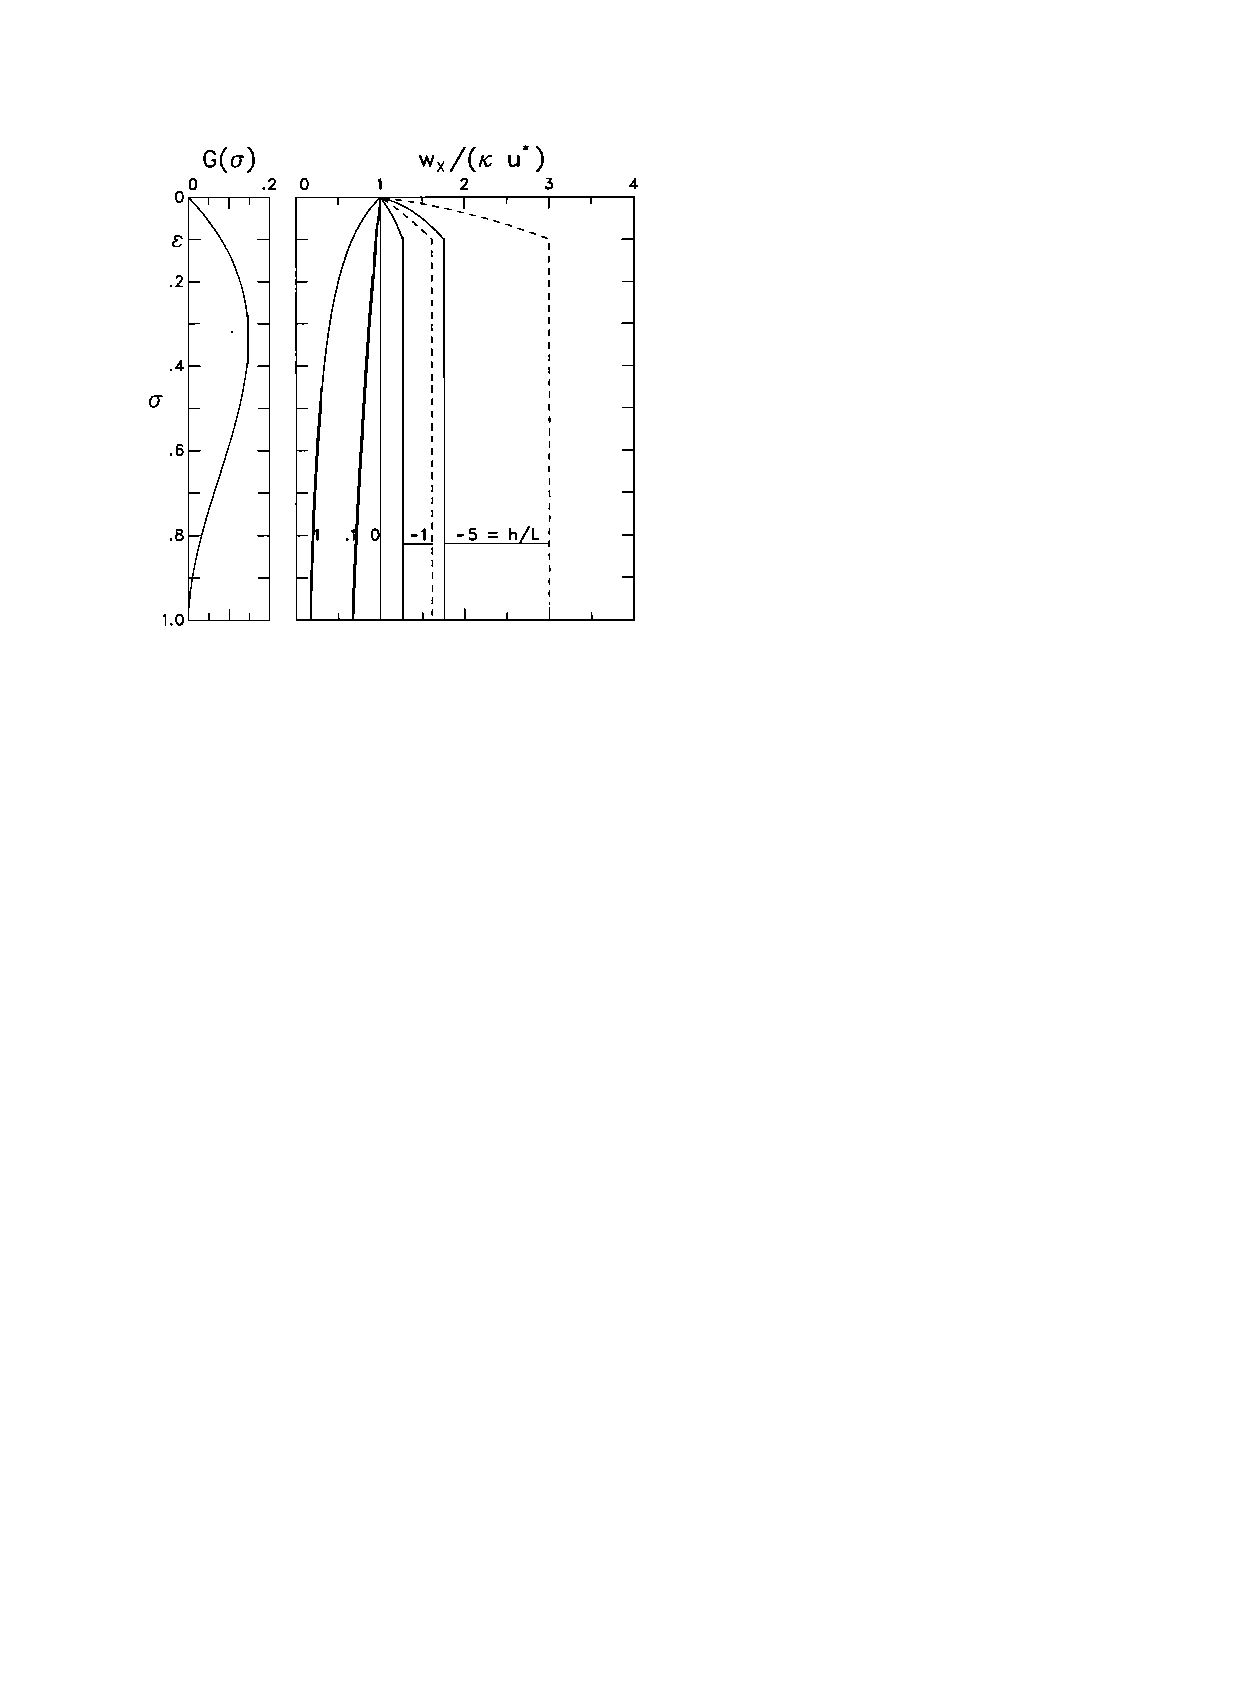
\includegraphics[angle=0,width=8cm]{./figs/LargeKPP_fig2.pdf}
\caption[Figure 2 from \cite{LargeKPP}]{ \sf This is a reproduction of
  Figure 2 from \cite{LargeKPP}.  The vertical axis is the
  dimensionless vertical coordinate $\sigma = d/h$ within the KPP
  boundary layer $0 \le \sigma \le 1$.  The left panel shows the
  vertical profile of the shape or shape function,
  $G_{\lambda}(\sigma)$, used to scale the vertical diffusivity via
  equation (\ref{eq:kpp-diffusivity-again}).  The analytic form shown
  here is given by the universal form (equation
  (\ref{eq:universal-non-local-structure})) $G_{\mbox{\tiny
      universal}}(\sigma) = \sigma \, (1-\sigma)^{2}$ which
  corresponds to the \cite{Troen_Mahrt1986} form and which is
  independent of the quantity $\Lambda$ being diffused.  This is the
  form recommended for CVMix use.  \cite{LargeKPP} chose a more
  general form, based on the desire to match boundary layer
  diffusivities to interior diffusivities in which case the shape
  function becomes a function of $\lambda$.  We detail the problems
  with this general approach in Section
  \ref{subsection:kpp-shape-function}.  The right panel shows various
  examples of the normalized turbulent velocity scale $w_{\lambda}$
  (called $w_{x}$ in \cite{LargeKPP}), with the examples differing by
  the value of the dimensionless ratio $h/L$ between the boundary
  layer depth, $h$, and the Monin-Obukhov length scale $L$.  For
  unstable buoyancy forcing, $L<0$, the velocity scale for scalars,
  $w_{s}$ (dashed lines), is greater than that for momentum, $w_{m}$
  (solid lines).  For stable forcing, $L>0$, and both scalar and
  momentum have the same turbulent velocity scales, $w_{s} = w_{m}$.
  In general, the turbulent velocity scale is enhanced with unstable
  surface buoyancy forcing, and reduced with stable buoyancy forcing.}
\label{fig:kpp-figure2-reproduced}
\end{center}
\rule{\textwidth}{0.005in}
\end{figure}
%%%%%%%%%%%%%%%%%%%%%%%%%%%%%%%%%%%%%%%%%%%%%%%%%%%%%%%%%%%%%%%%%%%%%%%%



\subsection{Similarity functions $\phi_{\Lambda}$}
\label{subsection:similarity-functions}

The vertical velocity scales are functions of the similarity functions
$\phi_{\Lambda}$, also called the dimensionless flux profiles.
Appendix B of \cite{LargeKPP} present analytic forms for these
functions, based on fits to available data, with their Figure B1
(reproduced here as Figure \ref{fig:large-etal-figureB1}) providing a
summary of the choices for the momentum function $\phi_{m}$ and the
scalar function $\phi_{s}$.  Both functions agree for stable buoyancy
forcing, in which they depend linearly on the dimensionless
Monin-Obukhov length $\zeta = d/L = \sigma \, h/L$.  We now discuss
the more complex case of unstable buoyancy forcing.


\subsubsection{The \cite{LargeKPP} choices for unstable buoyancy forcing}

For unstable buoyancy forcing, where $L<0$ and so $\zeta < 0$, there
are two regimes.  The scalar function $\phi_{s}$ is always less than
the momentum function $\phi_{m}$.  Hence, for unstable forcing there
is a larger turbulent velocity scale for the scalars than momentum
($w_{s} > w_{m}$), and thus a larger vertical diffusivity for scalars
than momentum ($K_{s} > K_{m}$).  The turbulent Prandtl number,
$\mbox{Pr}$, is given by the ratio of the flux functions
\begin{equation}
  \mbox{Pr} = \frac{K_{m}}{K_{s}} = \frac{w_{m}}{w_{s}} = \frac{\phi_{m}}{\phi_{s}}.
\label{eq:prandtl-number}
\end{equation}
The choices made by \cite{LargeKPP} lead to a Prandtl number in the
convective limit ($\zeta \rightarrow -\infty$) of 
\begin{equation}
 \mbox{Pr}  \rightarrow \left( \frac{c_{m}}{c_{s}} \right)^{1/3} = 0.44.
\label{eq:convective-limit-prandtl}
\end{equation}
The coefficients $c_{m}$ and $c_{s}$ are parameters in the similarity
functions $\phi_{m}$ and $\phi_{s}$, respectively.  Assuming the forms
for the similarity functions given by \cite{LargeKPP}, their Appendix
B suggests the following values
\begin{subequations}
\begin{align}
  c_{s} &=  98.96 \\
\label{eq:cs-defined}
  c_{m} &= 8.38.
\end{align}
\end{subequations}
If different forms for the similarity functions are used, such as
proposed in Section
\ref{subsubsection:alternative-similarity-functions}, then different
fit values will need to be used.


 
%%%%%%%%%%%%%%%%%%%% %%%%%%%%%%%%%%%%%%%%%%%%%
\begin{figure}[h!t]
\rule{\textwidth}{0.005in}
\begin{center}
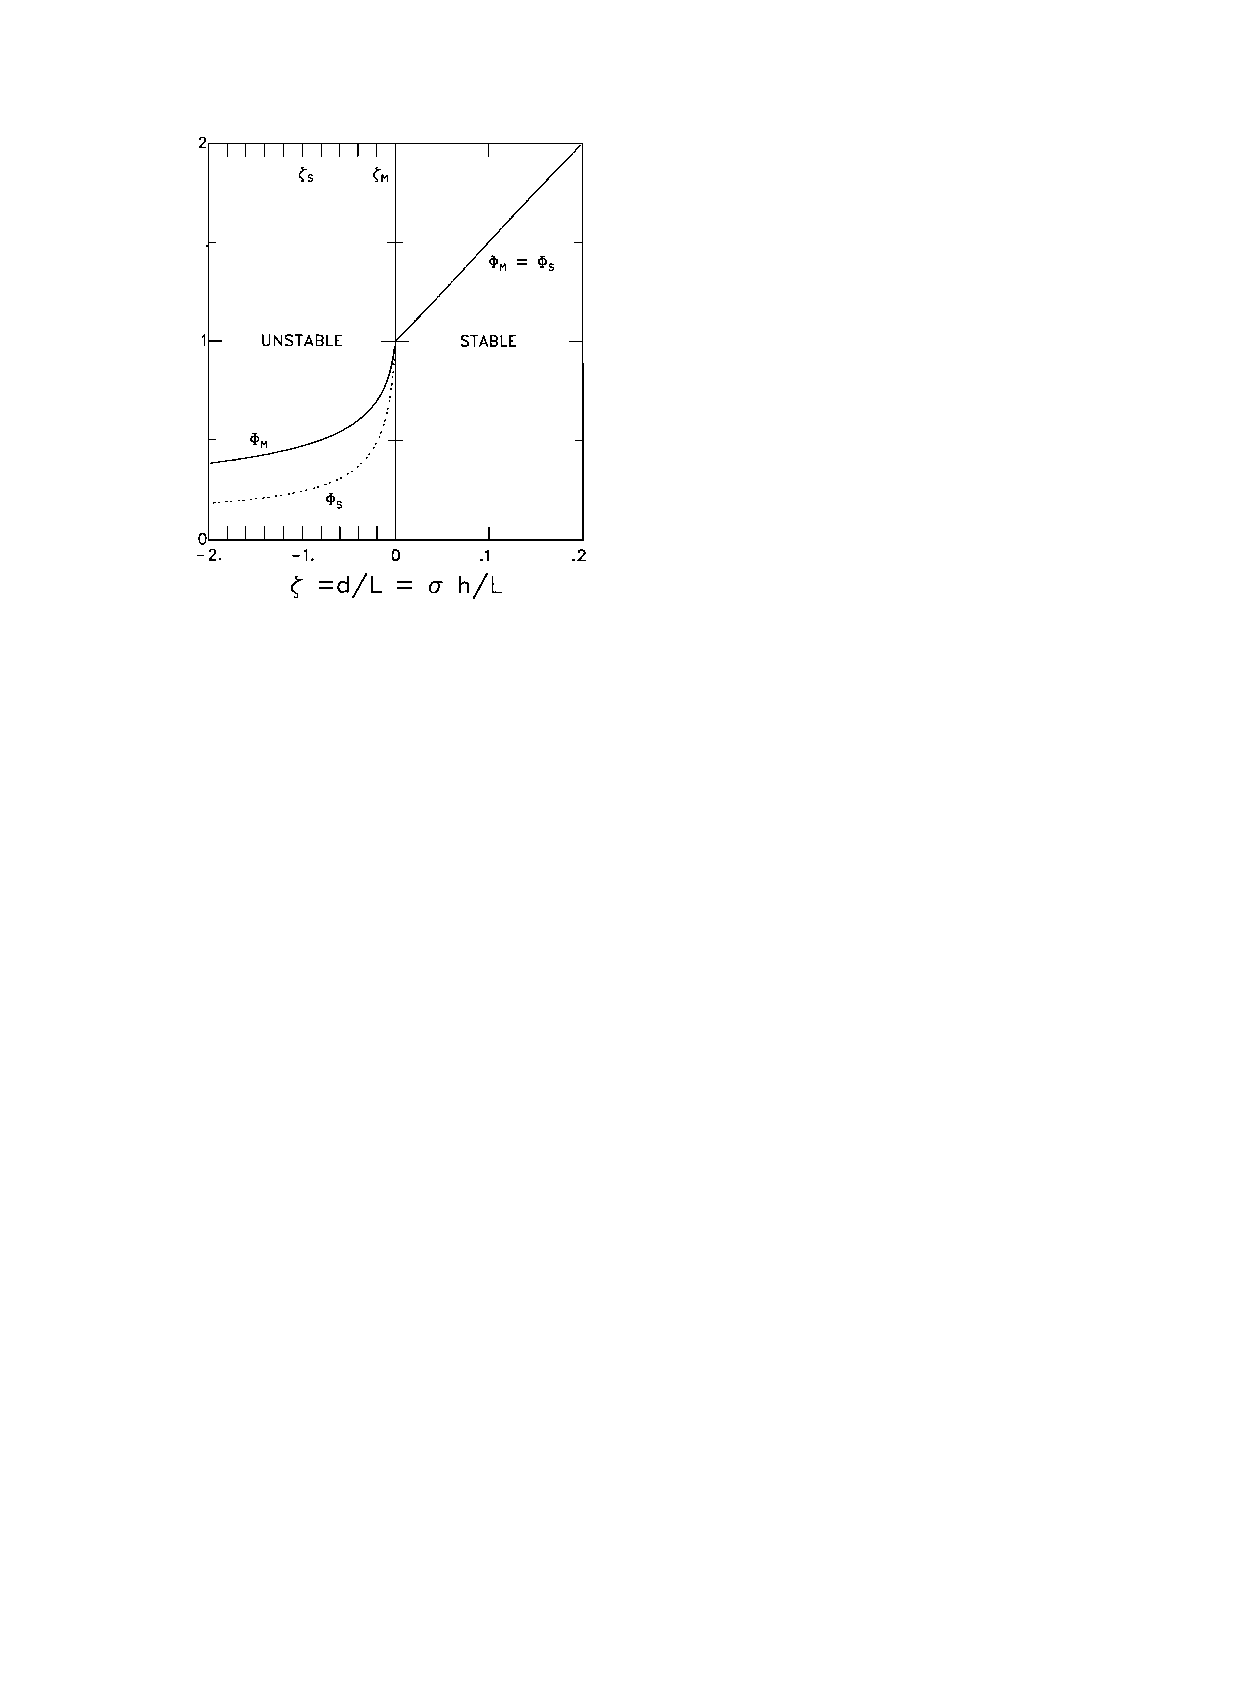
\includegraphics[angle=0,width=8cm]{./figs/LargeKPP_figB1.pdf}
\caption[Figure B1 from \cite{LargeKPP}]{\sf This is a reproduction of
  Figure B1 from \cite{LargeKPP}.  The vertical axis provides values
  for the dimensionless flux profiles, $\phi_{\Lambda}$, for momentum
  and scalars, and the horizontal axis gives the dimensionless
  Monin-Obukhov length scale $\zeta = d/L = \sigma \, h/L$.  There is
  a transition across the neutrally forced value of $\zeta = 0$.  For
  stable buoyancy forcing ($\zeta > 0$), both functions are the same,
  $\phi_{s} = \phi_{m}$, and are linear functions of $\zeta$. For
  unstable buoyancy forcing ($\zeta < 0$), the scalar function is less
  than momentum, $\phi_{s} < \phi_{m}$, with both functions falling
  off with a negative fractional power.  The analytic forms for the
  functions are given by equations (B1) and (B2) in \cite{LargeKPP}.}
\label{fig:large-etal-figureB1}
\end{center}
\rule{\textwidth}{0.005in}
\end{figure}
%%%%%%%%%%%%%%%%%%%%%%%%%%%%%%%%%%%%%%%%%%%%%%%%%%%%%%%%%%%%%%%%%%%%%%%%


\subsubsection{Alternative choices for unstable buoyancy forcing}
\label{subsubsection:alternative-similarity-functions}

\cite{LargeKPP} chose two regimes for the unstable buoyancy forced
range, transitioning from different fractional exponents near $\zeta =
0$, to the same $-1/3$ power for larger negative $\zeta$.  The scalar
function $\phi_{s}$ falls off faster near $\zeta=0$, with a power
$-1/2$, whereas the momentum function $\phi_{m}$ falls off with a
$-1/4$ power.  This initial distinct fractional power falloff sets the
scale for the Prandtl number in this portion of $\zeta$ in the weakly
unstable regime.

Having two regimes for the negative buoyancy forcing adds complexity
to the algorithm.  We thus consider how well the original two-regime
forms for $\phi_{m}$ and $\phi_{s}$ can be fit using a single regime,
using only the fractional power $-1/3$.  Tests suggest that the
following forms may be suitable
\begin{equation}
   \phi_{m}(\zeta) = \left\{
 \begin{array}{lll}
  &1 + 5 \, \zeta      &\zeta > 0 \\
  &(1-9\zeta)^{-1/3}  &\zeta < 0 
 \end{array}
 \right.
\label{eq:phim-alternative}
\end{equation}
\begin{equation}
   \phi_{s}(\zeta) = \left\{
 \begin{array}{lll}
  &1 + 5 \, \zeta      &\zeta > 0 \\
  &(1-60\zeta)^{-1/3}  &\zeta < 0. 
 \end{array}
 \right.
\label{eq:phis-alternative}
\end{equation}
A comparison of the original forms from \cite{LargeKPP} to the
alternative forms is shown in Figure
\ref{fig:phi-alternative-kpp}. Also shown is the ratio of these two
functions which yields the turbulent Prandtl number according to
equation (\ref{eq:prandtl-number}).  The agreement between the
original forms and the new forms is worse when considering the Prandtl
number.  As discussed in the figure caption, a viable means for
simplifying the turbulent functions, without compromising much on the
values used in \cite{LargeKPP}, is to maintain original 3-region
$\phi_{s}$ form, but to simplify $\phi_{m}$ to 2-regions according to
equation (\ref{eq:phim-alternative}).

The simplified forms for the similarity functions $\phi_{s}$ and
$\phi_{m}$ have {\it not} been implemented in CVMix.  More testing is
required.


%%%%%%%%%%%%%%%%%%%% %%%%%%%%%%%%%%%%%%%%%%%%%
\begin{figure}[h!t]
\rule{\textwidth}{0.005in}
\begin{center}
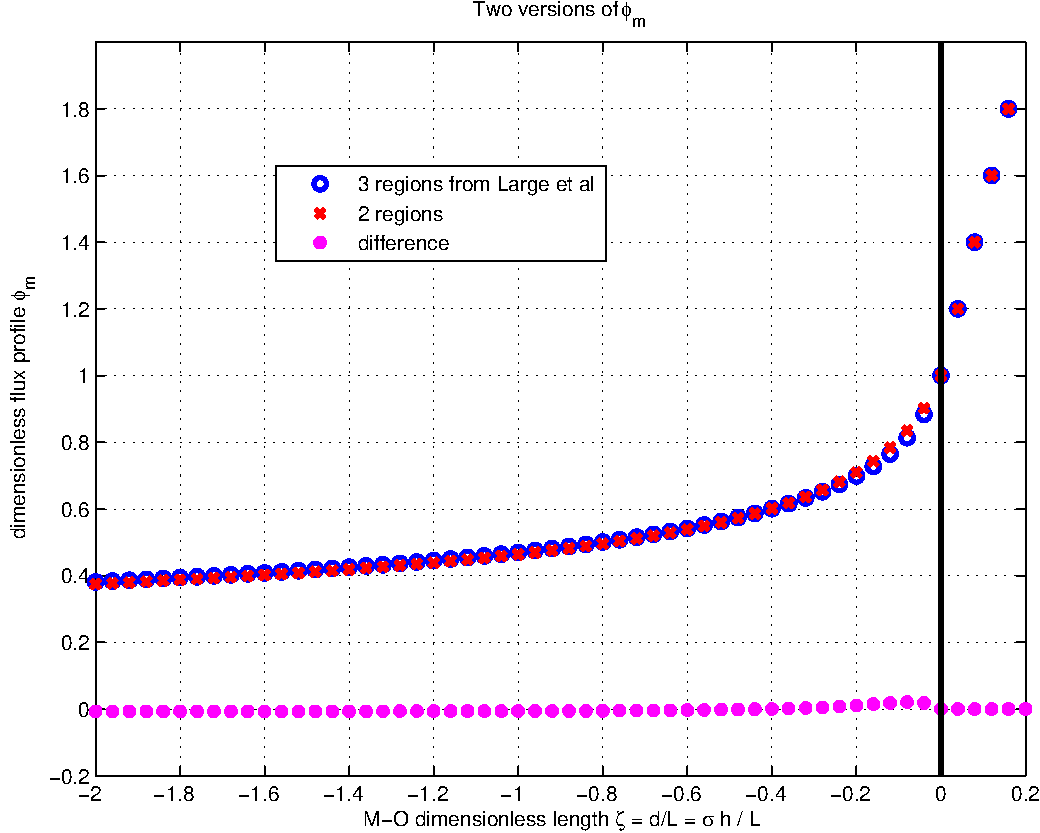
\includegraphics[angle=0,width=8cm]{./figs/phi_m_profiles.pdf}
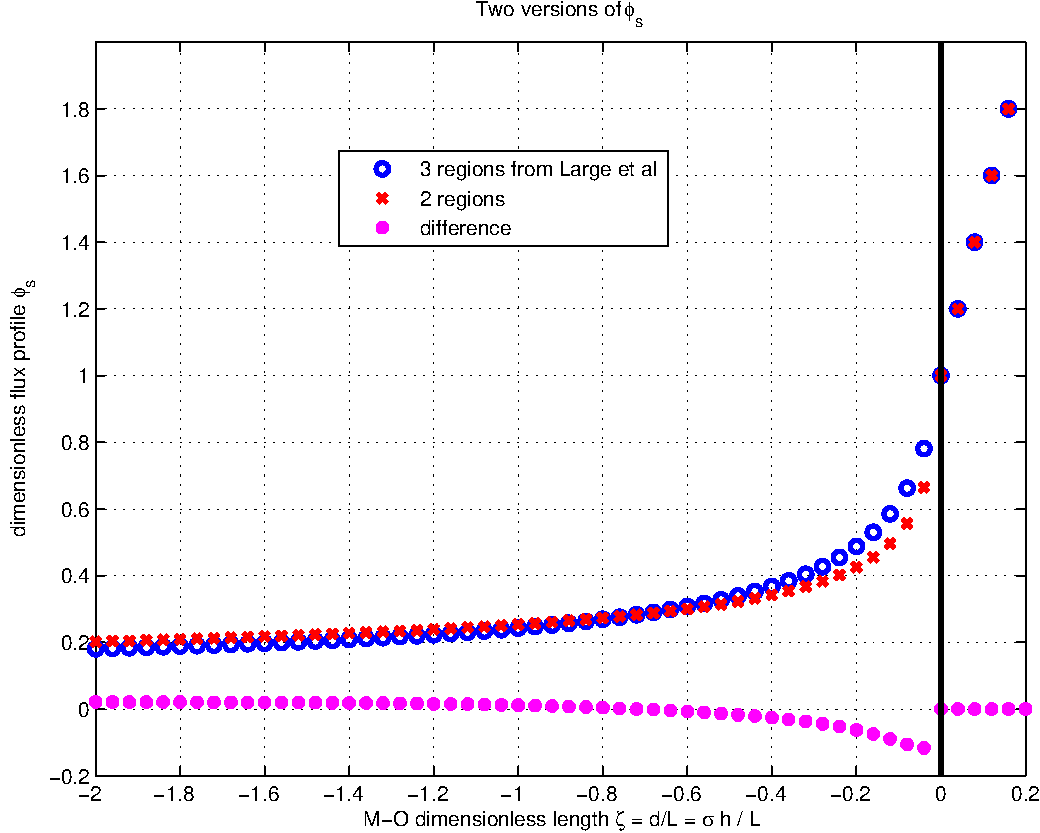
\includegraphics[angle=0,width=8cm]{./figs/phi_s_profiles.pdf}
\\
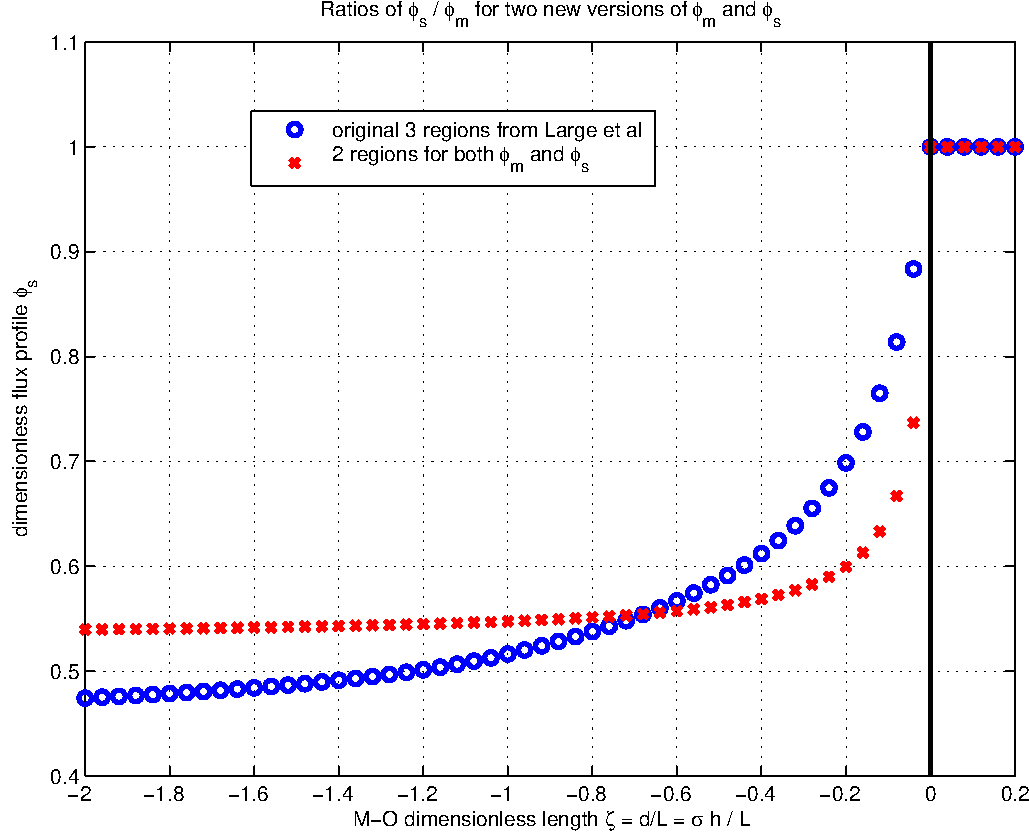
\includegraphics[angle=0,width=8cm]{./figs/prandtl_profiles_phim_phis.pdf}
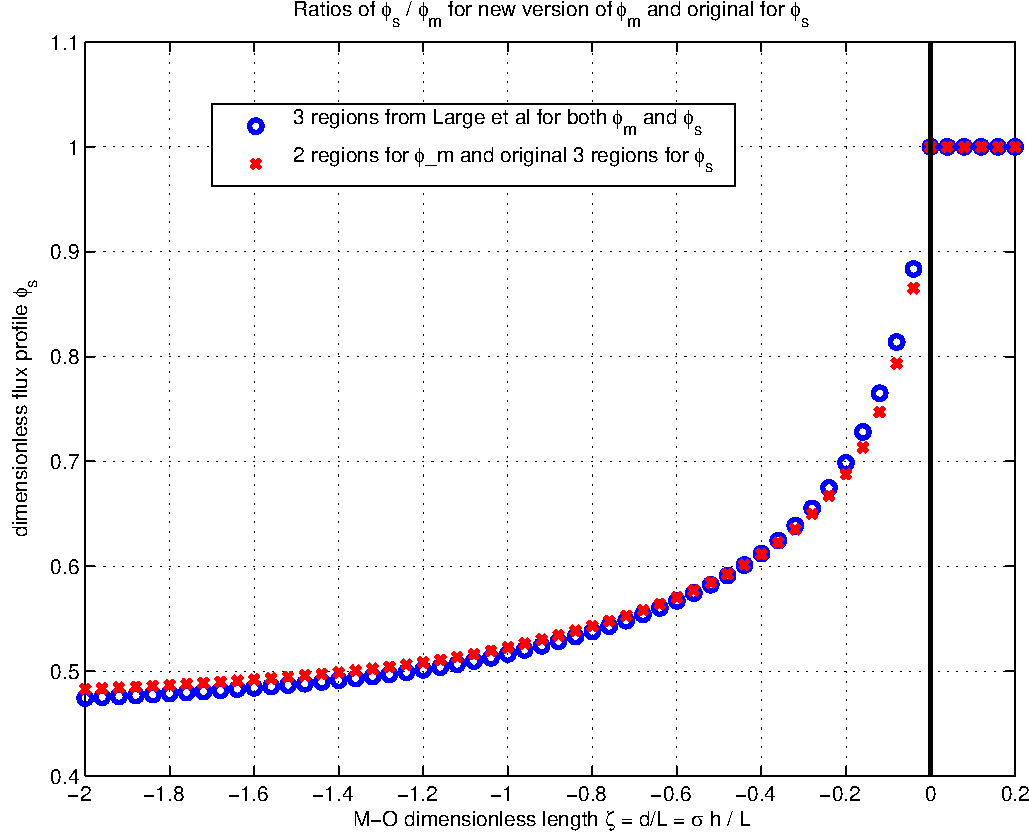
\includegraphics[angle=0,width=8cm]{./figs/prandtl_profiles_just_phim_new.pdf}
\caption[Alternative similarity functions]{\sf Shown here are 2-region
  flux profiles given by equations (\ref{eq:phim-alternative}) and
  (\ref{eq:phis-alternative}) as compared to the original 3-region
  profiles rom \cite{LargeKPP}.  We also show the ratio,
  $\phi_{s}/\phi_{m}$, which defines the turbulent Prandtl number or
  the ratio of the vertical momentum viscosity to vertical tracer
  diffusivity.  The top left panel shows the original 3-region
  $\phi_{m}$ as compared to the 2-region form
  (\ref{eq:phim-alternative}).  The agreement is quite close.  The top
  right panel shows the comparison for $\phi_{s}$, with the agreement
  not very good. The lower left panel shows the ratio
  $\phi_{s}/\phi_{m}$ for the original 3-region functions and the new
  2-region functions.  Their ratio amplifies the problems with the new
  $\phi_{s}$ form (\ref{eq:phis-alternative}).  The lower right panel
  shows the ratio of the original 3-region $\phi_{s}$ to the new
  2-region form of $\phi_{m}$.  These results suggest that to remain
  consistent with the original \cite{LargeKPP} results, it is feasible
  to switch to the 2-region form (\ref{eq:phim-alternative}) for
  $\phi_{m}$, but we must maintain the original 3-region form of
  $\phi_{s}$.}
\label{fig:phi-alternative-kpp}
\end{center}
\rule{\textwidth}{0.005in}
\end{figure}
%%%%%%%%%%%%%%%%%%%%%%%%%%%%%%%%%%%%%%%%%%%%%%%%%%%%%%%%%%%%%%%%%%%%%%%%


\subsection{The shape function $G_{\lambda}(\sigma)$ as per \cite{LargeKPP}}
\label{subsection:kpp-shape-function}

The vertical shape function $G_{\lambda}(\sigma)$ is given by the cubic
polynomial 
\begin{equation}
 G_{\lambda}(\sigma) = a_{0} + a_{1} \, \sigma + a_{2} \, \sigma^{2} + a_{3} \, \sigma^{3}.
\label{eq:shape-function-gsigma-again}
\end{equation}
As already noted when introducing this cubic expression (equation
(\ref{eq:shape-function-gsigma})), turbulent eddies do not cross
the ocean surface at $\sigma=0$, so the diffusivity should vanish at
$\sigma=0$.  This constraint is satisfied by setting
\begin{equation}
 a_{0} = 0.
\end{equation}
We now discuss further constraints to specify the remaining
coefficients.  For this purpose, we follow the general approach from
\cite{LargeKPP}, in which the shape function is determined by matching
boundary layer diffusivity to the interior diffusivity.  It is this
matching that can lead to distinct shape functions for tracers, given
that the interior diffusivities can differ between tracers.  We
question this matching method in Section
\ref{subsection:kpp-shape-function-cvmix}, where we propose to use the
universal shape function given by equation
(\ref{eq:universal-non-local-structure}).



\subsubsection{Constraints arising from the surface boundary condition
at $\sigma=0$}

We start by rewriting the expression
(\ref{eq:specifying-shape-function}) that expresses the ratio of
turbulent fluxes within the surface layer to those at the surface
boundary 
\begin{equation}
  a_{1} + a_{2} \, \sigma = \left( \frac{ \overline{w \, \lambda}^{\sigma}}{\overline{w \, \lambda}^{0}} \right)
 \qquad  \mbox{surface layer: $0 \le \sigma \le \epsilon$.}
\label{eq:specifying-shape-function-again}
\end{equation}
Satisfying this relation at the ocean surface, $\sigma=0$, requires
\begin{equation}
 a_{1} = 1, 
\end{equation}
 so that 
\begin{equation}
  1 + a_{2} \, \sigma = \left( \frac{ \overline{w \, \lambda}^{\sigma}}{\overline{w \, \lambda}^{0}} \right)
 \qquad  \mbox{surface layer: $0 \le \sigma \le \epsilon$.}
\label{eq:specifying-shape-function-againB}
\end{equation}
Now define the ratio
\begin{equation}
  \beta_{\lambda} = \left( \frac{ \overline{w \, \lambda}^{\epsilon}}{\overline{w \, \lambda}^{0}} \right),
\label{eq:beta-lambda-defined}
\end{equation}
which is the ratio of the turbulent flux at the base of the surface
layer, $\sigma = \epsilon$, to the flux at the upper ocean interface,
$d = -z + \eta = 0$.  For atmospheric boundary layers,
\cite{Troen_Mahrt1986} set
\begin{equation}
 \beta_{\lambda}  = 2 \, \epsilon \qquad \mbox{atmospheric boundary layers,} 
\end{equation}
with $\epsilon=0.1$.  \cite{Troen_Mahrt1986} further assume both the
shape function and its first derivative vanish at the base of the
boundary layer, $\sigma=1$.  These assumptions lead to the cubic
expression valid for all fluctuating fields $\lambda$
\begin{equation}
 G_{\mbox{\tiny universal}}(\sigma) = \sigma \, (1-\sigma)^{2}   \qquad \mbox{for} \; \; G(\sigma=0) = G(\sigma=1) = G'(\sigma=1) = 0, 
\label{eq:simple-shape-function}
\end{equation}
with this function exhibited in the left panel of Figure
\ref{fig:kpp-figure2-reproduced}.  We return to this function in
Section \ref{subsection:kpp-shape-function-cvmix}, where we recommend
it be used for the CVMix implementation of KPP.  


\subsubsection{Constraints arising from matching at $\sigma=1$}

\cite{LargeKPP} also assume the surface layer is 10\% of the boundary
layer, so that 
\begin{equation}
 \epsilon = 0.1 \qquad \mbox{KPP scheme.}
\end{equation}
However, they consider a more general approach for the shape function.
The reason \cite{LargeKPP} wish to generalize the atmospheric approach
of \cite{Troen_Mahrt1986} is to allow surface ocean boundary layer
turbulence to be impacted by interior mixing, with this mixing
parameterized by downgradient vertical diffusion.  Such diffusion
generally introduces distinct diffusivities for tracers (e.g., double
diffusion) as well as for momentum (e.g., non-unit Prandtl number).
For these reasons, \cite{LargeKPP} propose to have both the
diffusivity and its vertical derivative match across the base of the
boundary layer at $\sigma=1$.  These two matching conditions lead to
constraints given by equation (18) in \cite{LargeKPP}, which in turn
leads to shape functions that are dependent on the field being
transported.  In practice, satisfying these matching conditions is not
straightforward in an ocean model given the difficulties of estimating
vertical derivatives of diffusivities.  We also note that matching to
nonzero interior diffusivities means that the non-local transport term
does not smoothing go to zero at the base of the mixed layer.  We
return to these points in Section
\ref{subsection:kpp-shape-function-cvmix}. For the meantime, we
continue to present the prescription as proposed by \cite{LargeKPP},
as this approach is that which has been implemented in the NCAR models
using KPP.

It is critical note that if we allow the interior mixing coefficients
to influence the KPP boundary layer diffusivities via the matching
conditions at $\sigma=1$, then the KPP calculation should be called
{\it after} the various methods used to compute interior diffusivities
(e.g., double diffusion, tide mixing, shear mixing).  This ordering is
reflected in the CVMix flow diagram in Figure
\ref{fig:vertical_mix_flow_cvmix}.  The alternative approach
recommended in Section \ref{subsection:kpp-shape-function-cvmix}
allows for arbitrary ordering of the diffusivity calculation.


\subsubsection{Vanishing derivative at $\sigma=1$}

Matching both the shape function and its vertical derivative across
the boundary layer base at $\sigma=1$ adds complexity to the KPP
algorithm.  Furthermore, it is unclear how accurate one can in fact
satisfy both matching conditions on a finite grid with potentially
coarse vertical spacing at the boundary layer base.  To simplify the
KPP algorithm, we drop the need to match the vertical derivative of
the diffusivity.  Instead, we assume continuity of the diffusivity
with a vanishing derivative at the boundary layer base, $\sigma=1$.
Setting $\partial_{\sigma} G(\sigma) = 0$ at $\sigma=1$ leads to the
relation
\begin{equation}
 \left( \frac{\partial  G(\sigma)}{\partial \sigma} \right)_{\sigma =1} = 0 \Longrightarrow   3 \, a_{3} = -(1+ 2 \, a_{2}). 
\label{eq:a3-in-terms-of-a2}
\end{equation}
Matching diffusivities at $\sigma=1$ between the boundary layer and
interior value leads to
\begin{equation}
  a_{2}  = -2 + \left(\frac{3 \, K_{\lambda}(h)}{h \, w_{\lambda}(h)}
  \right),
\label{eq:a2-specified}
\end{equation}
where the diffusivity $K_{\lambda}(h)$ is determined by
parameterizations of interior mixing.  Substituting this expression
for $a_{2}$ into equation (\ref{eq:a3-in-terms-of-a2}) for $a_{3}$
leads to
\begin{equation}
 a_{3} = 1 - \left(\frac{2 \, K_{\lambda}(h)}{h \, w_{\lambda}(h)} \right).
\end{equation}
The resulting form for $G_{\lambda}(\sigma)$ is given by 
\begin{equation}
  G_{\lambda}(\sigma) = \sigma \, (1-\sigma)^{2}+ \sigma^{2} \,  (3 - 2 \, \sigma) \, \left(\frac{K_{\lambda}(h)}{h \, w_{\lambda}(h)} \right)
  \qquad \mbox{for} \; \; G_{\lambda}(\sigma=0) = G_{\lambda}'(\sigma=1) = 0. 
\end{equation}
Notice how the shape function reduces to the simpler form
$G(\sigma) = \sigma \, (1-\sigma)^{2}$ when matching to a zero
diffusivity, $K_{\lambda}(h) = 0$, at the boundary layer base (see
equation (\ref{eq:simple-shape-function})).


\subsection{The non-local term $\gamma_{\lambda}$ as per \cite{LargeKPP}}
\label{subsection:kpp-non-local-transport}

We now consider the parameterization for the non-local transport (see
Section \ref{subsection:kpp-nonlocal-transport-outline}) as suggested
by \cite{LargeKPP}.  Again, the KPP parameterization takes the form
(equation (\ref{eq:kpp-parameterization}))
\begin{equation}
  \overline{w \, \lambda} = -K_{\lambda} \left( \frac{\partial \Lambda}{\partial z} - \gamma_{\lambda} \right),
\label{eq:kpp-parameterization-yet-again}
\end{equation}
where we set 
\begin{equation}
K^{\mbox{\tiny non-local}}_{\lambda} = K_{\lambda}.
\end{equation}
In this way, the non-local portion of the turbulent flux is
parameterized according to
\begin{equation}
 \overline{w \, \lambda}^{\mbox{\tiny non-local}} = K_{\lambda}  \, \gamma_{\lambda},  
\end{equation}
where $K_{\lambda}$ takes the form in equation
(\ref{eq:kpp-diffusivity-again}): 
\begin{equation}
 K_{\lambda}(\sigma) = h \, w_{\lambda}(\sigma) \, G_{\lambda}(\sigma).
\label{eq:kpp-diffusivity-yet-again}
\end{equation}
For completeness, we repeat elements of the outline presented in
Section \ref{subsection:kpp-nonlocal-transport-outline}.


\subsubsection{General features of $\gamma_{\lambda}$ with the KPP parameterization}
\label{subsubsection:general-features-gamma-as-per-largekpp}

\begin{itemize}

\item \cite{Smyth_etal2002} consider a non-local term for momentum.
  Until their ideas have been fully tested in climate models, we
  follow recommendations from \citep{LargeKPP}, who set the non-local
  momentum term to zero:
\begin{equation}
 \gamma_{\lambda} \; \; = \; \; 
\left\{
 \begin{array}{ll}
  0 \; \;  &\mbox{if $\lambda = (u,v,w)$ a velocity component}
 \\
  \ne 0 \; \; &\mbox{nonzero if $\lambda = \theta,s$ or another tracer.}
  \end{array}
 \right.
\end{equation}

  \item The non-local transport is non-zero only within the OBL:  
\begin{equation}
 \gamma_{\lambda} \; \; = \; \; 
  \left\{ 
  \begin{array}{ll}
   0 \; \; &\mbox{if $\sigma > 1$}
   \\ 
   \ne 0  \; \; &\mbox{if $0 \le \sigma \le 1$.}
  \end{array}
 \right.
\end{equation}

  \item The non-local transport is non-zero only in the presence of
    destabilizing negative surface ocean buoyancy flux:
\begin{equation}
 \gamma_{\lambda} \; \; = \; \; 
  \left\{ 
  \begin{array}{ll}
   0 \; \; &\mbox{for $B_{f} > 0$}
   \\ 
   \ne 0 \; \; &\mbox{for $B_{f} < 0$.}
  \end{array}
 \right.
\end{equation}


\item The non-local transport for temperature and arbitrary scalars is
  given by the following form for destabilizing negative surface ocean
  buoyancy fluxes:
\begin{align}
 \gamma_{\theta} &= 
   C_{s} \, \left( \frac{ \overline{w \, \theta}^{0} - Q_{R}/(\rho_{o} \, C_{\mbox{\tiny p}}^{o})  }{h \,  w_{\theta}(\sigma)}  
            \right) 
\label{eq:non-local-temp-kpp}
\\
 \gamma_{s} &= 
   C_{s} \, \left( \frac{ \overline{w \, s}^{0} }{h \,  w_{s}(\sigma)}  
            \right), 
\label{eq:non-local-scalar-kpp}
\end{align}
 where 
\begin{equation}
 C_{s} = C_{*} \, \kappa \, (c_{s} \, \kappa \, \epsilon)^{1/3},  
\label{eq:cs-and-cstar-defined}
\end{equation}
with 
\begin{equation}
 C_{*} = 10,
\label{eq:cstar-value-specified}
\end{equation}
and $Q_{R}$ is the heat flux from penetrative radiation given by
equation (\ref{eq:penetrative-heating-kpp}).  We have more to say in
Section \ref{subsection:penetrative-radiation-and-kpp-nonlocal}
regarding the shortwave flux, $Q_{R}$, and the non-local term.  We
argue in that section that the shortwave flux should {\it not} be part
of the non-local term.  However, for the meantime we continue
following the approach of \cite{LargeKPP}, in which they include
shortwave radiation as part of the non-local term (e.g., see equation
(20) in \cite{LargeKPP}).  Note that equation
(\ref{eq:non-local-temp-kpp}) uses $c_{s}$ regardless of the scalar
tracer field considered.

\end{itemize}

Combining the parameterizations (\ref{eq:non-local-temp-kpp}) and
(\ref{eq:non-local-scalar-kpp}) for the non-local term
$\gamma_{\lambda}$, with that for the vertical diffusivity
$K_{\lambda}$ in equation (\ref{eq:kpp-diffusivity-yet-again}) renders
the non-local flux parameterization in the form
\begin{align}
\overline{w \, \theta}^{\mbox{\tiny non-local}} &= K_{\theta}  \, \gamma_{\theta}
  = 
 G_{\theta}(\sigma) \, C_{s} \, \left( \overline{w \, \theta}^{0} - Q_{R}/(\rho_{o} \, C_{\mbox{\tiny p}}^{o}) \right)
\label{eq:non-local-flux-kpp-param-temp}
\\
\overline{w \, s}^{\mbox{\tiny non-local}} &= K_{s}  \, \gamma_{s}
  = 
 G_{s}(\sigma) \, C_{s}\,\left( \overline{w \, s}^{0} \right).
\label{eq:non-local-flux-kpp-param-scalar}
\end{align}
Notice how explicit dependence on both the turbulent velocity scale,
$w_{\lambda}$, and boundary layer depth, $h$, drop out from the
parameterization of the non-local flux.  The expressions
(\ref{eq:non-local-flux-kpp-param-temp}) and
(\ref{eq:non-local-flux-kpp-param-scalar}) exhibit clearly how the
non-local transport provides a redistribution of the surface boundary
flux into the boundary layer. This redistribution is analogous to the
penetrative radiation associated with shortwave. 



\subsubsection{Summary of the non-local transport parameterization} 

We now summarize the non-local transport for temperature and arbitrary
scalars, with \cite{LargeKPP} proposing a parameterization according
to the following expression, again valid just for destabilizing
negative surface ocean buoyancy fluxes (it vanishes for stable
buoyancy forcing):
\begin{align}
 \gamma_{\theta} &= 
   C_{s} \, \left( \frac{ \overline{w \, \theta}^{0} - Q_{R}/(\rho_{o} \, C_{\mbox{\tiny p}}^{o} )  }{h \,  w_{\theta}(\sigma)}  
            \right) 
\label{eq:non-local-temp-kpp-again}
\\
 \gamma_{s} &= 
   C_{s} \, \left( \frac{ \overline{w \, s}^{0} }{h \,  w_{s}(\sigma)}  
            \right).
\label{eq:non-local-scalar-kpp-again}
\end{align}
In these expressions, we have (equation
(\ref{eq:cs-and-cstar-defined}))
\begin{equation}
 C_{s} = C_{*} \, \kappa \, (c_{s} \, \kappa \, \epsilon)^{1/3},  
\end{equation}
with \cite{LargeKPP} suggesting the value of 
\begin{equation}
 C_{*} = 10,
\end{equation}
whereas $C_{*} = 5$ in \cite{Smyth_etal2002}.  The von Karman constant
$\kappa = 0.40$ (equation (\ref{eq:von-karman-constant})) appears in
this expresion, as well as the fraction of the boundary layer assumed
to be occupied by the Monin-Obukhov surface layer
\begin{equation}
\epsilon = 0.1.
\end{equation}
The coefficient $c_{s} = 98.96$ (equation (\ref{eq:cs-defined}) is set
according to the similarity function $\phi_{s}$ (Section
\ref{subsection:similarity-functions}).  Plugging in the constants
suggested by \cite{LargeKPP} leads to
\begin{equation}
 C_{s} \approx 6.33. 
\label{eq:Cs-value}
\end{equation}

The flux $Q_{R}>0$ appearing
in the $\gamma_{\theta}$ expression for equation
(\ref{eq:non-local-temp-kpp-again}) is the heat flux crossing the
ocean surface from shortwave radiation.  We split this penetrative
shortwave flux from the non-penetrative heat flux $\overline{w \,
  \theta}^{0}$, which is positive for cases where heat leaves the
ocean surface due to non-penetrative heat fluxes (i.e., longwave,
sensible, and latent).  The net heat flux crossing the ocean surface
is given by
\begin{subequations}
\begin{align}
 Q^{\mbox{\scriptsize heat}} &= Q_{R} - \rho_{o} \, C_{\mbox{\tiny p}}^{o} \,  \overline{w \, \theta}^{0},
\label{eq:heat-flux-penetrative-and-non-penetrative}
 \\
 &=  Q_{R} + C_{\mbox{\tiny p}}^{o} \,  Q_{\theta}^{\mbox{\tiny non-pen}},
\end{align}
\end{subequations}
where $Q^{\mbox{\scriptsize heat}} > 0$ for heat entering the ocean,
and $C_{\mbox{\tiny p}}^{o} \, Q_{\theta}^{\mbox{\tiny non-pen}}$ is
the non-penetrative heat fluxes arising from longwave, latent, and
sensible heating (Section \ref{subsection:non-pen-buoyancy-fluxes}).
The parameterized non-local transport term thus takes the following
form for temperature
\begin{equation}
 \gamma_{\theta} = -\left(\frac{ C_{s}}{\rho_{o}  \, C_{\mbox{\tiny p}}^{o} } \right) 
  \frac{ Q^{\mbox{\scriptsize heat}} }{h \,  w_{\theta}(\sigma)}.  
\label{eq:non-local-temp-kpp-again-again}
\end{equation}
Generally the negative buoyancy forcing that gives rise to the
non-local transport is associated with cooling
($Q^{\mbox{\scriptsize heat}} < 0$), so that 
\begin{equation}
  \gamma_{\theta} > 0 \qquad \mbox{surface cooling}.
\label{eq:surface-cooling-gamma-theta}
\end{equation}
Similar considerations lead to the non-local transport term for
scalars such as salt 
\begin{equation}
 \gamma_{s} = -C_{s} \, \left( \frac{ Q^{s}  }{h \,  w_{s}(\sigma)} \right),  
\label{eq:non-local-scalar-kpp-again-again}
\end{equation}
where $Q^{s} > 0$ when scalar enters through the ocean surface
(Section \ref{subsection:conventions}).

Combining the parameterizations
(\ref{eq:non-local-temp-kpp-again-again}) and
(\ref{eq:non-local-scalar-kpp-again}) for the non-local term
$\gamma_{\lambda}$, with that for the vertical diffusivity
$K_{\lambda}$ in equation (\ref{eq:kpp-diffusivity}) renders the
non-local flux parameterization for temperature and an arbitrary
scalar in the form (again, $B_{f} < 0$ for non-zero non-local
transport)
\begin{subequations}
\begin{align}
\overline{w \, \theta}^{\mbox{\tiny non-local}} &= K_{\theta}  \, \gamma_{\theta}
  = 
 - G_{\theta}(\sigma) \, C_{s} \, \left( \frac{ Q^{\mbox{\scriptsize heat}}}{ \rho_{o}  \, C_{\mbox{\tiny p}}^{o} } \right)
\label{eq:non-local-flux-kpp-param-temp-again}
\\
\overline{w \, s}^{\mbox{\tiny non-local}} &= K_{s}  \, \gamma_{s}
  = 
 -G_{s}(\sigma) \, C_{s} \,  Q^{s}.
\label{eq:non-local-flux-kpp-param-scalar-again}
\end{align}
\end{subequations}
Notice how explicit dependence on both the turbulent velocity scale,
$w_{\lambda}$, and boundary layer depth, $h$, drop out from the
parameterization of the non-local flux.  For the CVMix implementation
of the non-local transport, the CVMix code computes the products
$G_{\theta}(\sigma) \, C_{s}$ and $G_{s}(\sigma) \, C_{s}$, and
returns them to the calling model, which then computes the non-local
flux upon multiplication by the boundary flux.  In this way we see
explicitly how the non-local transport provides a redistribution of
the surface boundary flux into the boundary layer.


\subsection{The shape function and non-local transport: Part I}
\label{subsection:kpp-shape-function-cvmix}

The discussion of the shape function $G_{\lambda}(\sigma)$ in Section
\ref{subsection:kpp-shape-function} and the non-local term
$\gamma_{\lambda}$ in Section \ref{subsection:kpp-non-local-transport}
follow the general prescription from \cite{LargeKPP}.  However, there
are problems with this prescription related to the non-local transport
that motivate use of the universal shape function
(\ref{eq:universal-non-local-structure}) for the diffusivity
$K_{\lambda} = K^{\mbox{\tiny non-local}}_{\lambda}$.



\subsubsection{Problem I: non-local flux larger than surface flux}
\label{subsubsection:non-local-flux-too-large}

The first problem with the \cite{LargeKPP} prescription relates to
cases where the parameteried non-local flux,
(\ref{eq:non-local-flux-kpp-param-temp}) of
(\ref{eq:non-local-flux-kpp-param-scalar}), is larger than the surface
tracer flux
\begin{equation}
   G_{\lambda}(\sigma) \, C_{s} > 1\qquad \mbox{non-local flux greater than surface flux.}
\end{equation}
The non-local transport is meant to redistribute the surface flux
through the boundary layer.  However, values for $G_{\lambda}(\sigma)
\, C_{s} > 1$ mean the non-local flux is itself larger than the
surface boundary flux.  Experience has shown that one may realize
$G_{\lambda}(\sigma) \, C_{s} > 1$ near the boundary layer base,
$\sigma=1$, when the interior diffusivity is relatively large.  The
matching conditions employed by \cite{LargeKPP} (Section
\ref{subsection:kpp-shape-function}) then lead to a relatively large
value for the shape function $G_{\lambda}(\sigma)$.  In this case, one
may be exposed to the production of extrema in the tracer field.  In
the presence of sea-ice, problems may arise particularly in fresh
water regions such as the Baltic Sea where the thermal expansion
coefficient is negative, $\alpha < 0$ (Martin Schmidt, personal
communication).

The following modifications to the original \cite{LargeKPP} scheme
have been found useful to reduce the potential for realizing
$G_{\lambda}(\sigma) \, C_{s} > 1$.
\begin{itemize}

\item {\sc interior gravitational instabilities}: When the vertical
  stratification is unstable ($N^{2} < 0$), vertical diffusivity is
  enhanced to remove the gravitational instability. Notably, it is
  {\it not} appropriate to enhance the diffusivity within the KPP
  boundary layer, beyond that already computed via the KPP scheme,
  even when $N^{2} < 0$.  On those occasions when the instabilities
  appear beneath the boundary layer, diffusivities are enhanced.  If
  one insisted that such diffusivities should match those in the
  boundary layer, then the shape function $G_{\lambda}(\sigma)$ would
  indeed become quite large in magnitude, thus leading to $
  G_{\lambda}(\sigma) \, C_{s} > 1$.  Hence, NCAR recommends that one
  pull the ``convective adjustment'' portion of the mixing scheme
  outside of the KPP portion of the algorithm.  That is, the interior
  convective instability diffusivities are {\it not} matched to the
  KPP boundary layer diffusivities.  This is the key reason that NCAR
  implements KPP prior to the calculation of diffusivities arising
  from gravitational instabilities.

\item {\sc simpler matching}: As noted in Section
  \ref{subsection:kpp-shape-function}, one may choose to simplify the
  matching at the boundary layer base.  The simpler approach assumes
  that only the diffusivities match across the boundary layer base,
  rather than also insisting on the derivative of the diffusivities as
  proposed by \cite{LargeKPP}.  The simplified matching condition
  leads to less problems computing discrete vertical derivatives of
  the diffusivities, and in turn produces more well regularized
  diffusivities and shape functions.  This approach has not been fully
  tested, but is compelling in theory.

\end{itemize}


\subsubsection{Problem II: spuriously large divergence}

By definition, the non-local transport vanishes beneath the boundary
layer where $\sigma >1$.  However, the diffusivity generally does not
vanish beneath the boundary layer.  Hence, by determining the shape
function $G_{\lambda}(\sigma)$ according to the needs of diffusivity
matching, then the non-local transport will in turn have a jump at the
boundary layer base.  Only for those cases where the interior
diffusivity vanishes will both the diffusivity and the non-local
transport have a smooth transition from the boundary layer into the
interior.

The jump in the non-local transport is unphysical, and it is a problem
exacerbated in the following situations.
\begin{itemize}

\item In relatively shallow waters where bottom induced mixing from
  tides may produce a sizable diffusivity reaching into the boundary
  layer, then the matching condition will create a relatively large
  value for $G_{\lambda}(\sigma) \, C_{s}$ at the boundary layer base,
  thus enhancing the jump across the boundary layer base. 

\item Refining the vertical grid spacing increases the magnitude of
  the divergence at the boundary layer base.

\end{itemize}


\subsubsection{Resolution I: two shape functions}

The fundamental problem is that the non-local transport
parameterization proposed by \cite{LargeKPP} does not smoothly
approach zero at the boundary layer base in those cases where the
interior diffusivity is nonzero.  Its adverse effects may be mild for
models with either small interior diffusivities or with coarse
vertical grid spacing.  However, modern global models, and many
regional models, are pushing the limits where interior mixing is
sizable and vertical grid spacing refined.

One solution to this problem is to use two distinct structure
functions: one for the diffusivity $K_{\lambda}$ and another for
$K^{\mbox{\tiny non-local}}_{\lambda}$.  The $K_{\lambda}$ shape
function, $G_{\lambda}(\sigma)$ will remain as originally proposed by
\cite{LargeKPP}, with matching to the interior diffusivity along with
the caveats noted above.  However, for the non-local transport, we
propose to use the cubic function (\ref{eq:simple-shape-function}) for
{\it all} tracers
\begin{equation}
G_{\mbox{\tiny universal}}(\sigma)= \sigma \, (1-\sigma)^{2}   \qquad \mbox{for} \; \; \sigma \le 1. 
\label{eq:universal-non-local-structure}
\end{equation}
As noted in the discussion of equation
(\ref{eq:simple-shape-function}) (see also Figure
\ref{fig:kpp-figure2-reproduced}), this shape function arises from
matching the function and its derivative to zero at the boundary layer
base.  This shape function removes problems with the spuriously large
divergences across the boundary layer base since the non-local term
smoothly goes to zero at $\sigma =1$.  Additionally, the shape
function $G_{\mbox{\tiny universal}}(\sigma)$ has a maximum at $\sigma
= 1/3$, where $G_{\mbox{\tiny universal}}'(\sigma) = 1 -4\sigma +
3\sigma^2 = 0$.  Hence, the maximum value for the product
$G_{\mbox{\tiny universal}}(\sigma) \, C_{s}$ is
\begin{equation}
 \left[ G_{\mbox{\tiny universal}}(\sigma=1/3) \, C_{s} \right]^{\mbox{\tiny maximum}} =  \left( \frac{4}{27}  \right) \, 6.33 \approx 0.94 < 1, 
\end{equation}
using $C_{s} = 6.33$ suggested by \cite{LargeKPP} (see equation
(\ref{eq:Cs-value})).  Since $\left[ G_{\mbox{\tiny
      universal}}(\sigma=1/3) \, C_{s} \right]^{\mbox{\tiny maximum}}
< 1$, the shape function $G_{\mbox{\tiny universal}}(\sigma)$ removes
problems with the non-local flux being larger than the surface flux.


\subsubsection{Resolution II: universal shape function}

The recommended approach for CVMix is to employ the {\it same} shape
function for the diffusivities as given by $G_{\mbox{\tiny
    universal}}(\sigma)= \sigma \, (1-\sigma)^{2}$ in equation
(\ref{eq:universal-non-local-structure}).  In this way, the KPP
diffusivity takes on the rather simple form for both the parameterized
local flux and non-local flux
\begin{equation}
 K^{\mbox{\tiny KPP}}_{\lambda}  = K_{\lambda}  =  K^{\mbox{\tiny non-local}}_{\lambda} = h \, w_{\lambda} \, \sigma \, (1-\sigma)^{2}.
\label{eq:universal-diffusivity}
\end{equation}
If this approach is used, then diffusivities from processes such as
tide mixing and shear mixing, which are not parameterized by the KPP
boundary layer scheme, should be allowed to penetrate into the surface
boundary layer.  That is, the approach proposed for CVMix assumes the
net diffusivity, even in the surface boundary layer, is the {\it sum}
of the KPP diffusivity plus that from other processes
\begin{equation}
 K_{\lambda}^{\mbox{\tiny net}} =  K^{\mbox{\tiny KPP}}_{\lambda} + \sum  K^{\mbox{\tiny other processes}}_{\lambda},
\label{eq:sum-of-diffusivities}
\end{equation}
where those other processes parameterized by the diffusivities
$K^{\mbox{\tiny other processes}}_{\lambda}$ are spectrally localized
away from the processes parameterized by KPP.  Again, this approach is
simpler than the original \cite{LargeKPP} approach, which incorporated
the effects from interior mixing by matching boundary layer and
interior diffusivities at the base of the boundary layer layer.  That
approach has serious problems in practice due to the reasons noted
earlier.  It also has no more fundamental physical basis than the
summed diffusivities (\ref{eq:sum-of-diffusivities}) proposed for
CVMix.

In summary, the recommended parameterization of the local and
non-local flux within the surface boundary layer via the KPP scheme is
given by
\begin{subequations}
\begin{align}
\overline{w \, \lambda}^{\mbox{\tiny local}} &= -K_{\Lambda}  \, \left( \frac{\partial \Lambda}{\partial z} \right)
 \\
\overline{w \, \theta}^{\mbox{\tiny non-local}} &= K_{\theta}  \, \gamma_{\theta} = 
 - \sigma \, (1-\sigma)^{2} \, C_{s} \, \left( \frac{ Q^{\mbox{\scriptsize heat}}}{ \rho_{o}  \, C_{\mbox{\tiny p}}^{o} } \right)
\label{eq:non-local-flux-kpp-param-temp-simple}
\\
\overline{w \, s}^{\mbox{\tiny non-local}} &= K_{s}  \, \gamma_{s}  = 
 -\sigma \, (1-\sigma)^{2}  \, C_{s} \,  Q^{s}.
\label{eq:non-local-flux-kpp-param-scalar-simple}
\end{align}
\end{subequations}
Since the vertical velocity scale $w_{\lambda}$ is the same for scalar
species, such as temperature, salinity, and biogeochemical species,
the KPP diffusivity is then the same for all tracers\footnote{The net
  tracer diffusivity within the surface boundary layer may be a
  function of the tracer, but tracer dependence arises only from
  processes that are not parameterized by the KPP scheme (see equation
  (\ref{eq:sum-of-diffusivities}).}
\begin{equation}
  K^{\mbox{\tiny KPP}}  = K_{\theta} = K_{s}.
\end{equation} 
The vertical viscosity arising from the KPP scheme generally differs
from the KPP tracer diffusivity, since the turbulent velocity scale
for momentum, $w_{m}$, differs from the tracer velocity scale, $w_{s}$
(see Sections \ref{subsection:vertical-velocity-scale} and
\ref{subsection:similarity-functions}).


\subsubsection{Further problems to be discussed later}

In section \ref{section:kernals-of-behaviour} we identify further
problems with the parameterized non-local term, even when using the
shape function $\sigma \, (1-\sigma)^{2}$.  We thus revisit in that
section the question about how to parameterize the non-local flux.


\subsection{Penetrative shortwave and the KPP non-local redistribution}
\label{subsection:penetrative-radiation-and-kpp-nonlocal}

Equation (20) from \cite{LargeKPP} provides an expression for the
non-local flux parameterized by KPP.  Notably, the heat flux includes
shortwave radiation.  In this section, we discuss some of the issues
related to the shortwave radiation and its contribution to the
non-local term.  We note that there is no guidance from the
atmospheric application of KPP, since the atmosphere is largely
transparent to shortwave.  In contrast, the ocean transmits surface
shortwave radiation only into a few 10s of metres of the upper ocean,
with the transmittance a function of the optical properties of
seawater.

The importance of penetrative shortwave radiation for upper ocean
heating, particularly in the tropics, is well established (e.g.,
\cite{Sweeneyetal}, \cite{Manizza_etal2005},
\cite{Anderson_color_etal2007}, \cite{Anderson_color_etal2009}).
Additionally, upper ocean shortwave heating plays an important role in
sea ice formation/melt in relatively fresh regions, such as the Baltic
Sea, where the thermal expansion coefficient, $\alpha$, is negative.
In these regions, shortwave heating, particularly in the spring time,
destabilizes the boundary layer (heating provides a negative buoyancy
flux when $\alpha < 0$), with the associated vertical mixing of warmer
sub-surface waters helping to melt the winter sea ice (Martin Schmidt,
personal communication).


\subsubsection{Physical ideas}
\label{subsubsection:shortwave-physics}

Recognizing that the KPP non-local term acts as a redistribution of
surface tracer fluxes, we are led to question whether the shortwave
heat flux should be included as part of the KPP surface heat flux
redistribution.  One may argue that it should {\it not} be included,
since it is already included as part of an optics-based penetration
process (e.g., \cite{Manizza_etal2005}), with this penetration
dependent only on seawater optical properties.  If we allow the
surface shortwave radiation to also be redistributed with the
non-local KPP process, then the net shortwave reaching beneath the
surface can be larger than the shortwave radiative flux incident on
the ocean surface.  But is this wrong?  And will it be problematic?
These are two related, but distinct, questions that we aim to address
here.

Consider a quiescent stably stratified ocean with uniform optical
properties; e.g., there is uniform chlorophyll concentration.
Shortwave radiation incident on the ocean surface will penetrate into
the interior according to the ocean optics, given some exponential
decay relations such as those from \cite{Manizza_etal2005}.  Now allow
the surface to have a strong cooling that is stronger than the
shortwave warming, thus creating a negative buoyancy flux and leading
to convective mixing processes.  Assuming uniform optical properties
both before and after the negative buoyancy flux means that the
exponential shortwave penetration remains unchanged.  However, the
shortwave absorbed in the surface layer ($\sigma < \epsilon \, h$)
will be carried into the deeper reaches of the boundary layer through
the action of the turbulence.  Consequently, there will be more
shortwave reaching the deeper portion of the boundary layer than just
through the optical penetration alone.  

We are thus motivated to include the shortwave radiation as part of
the surface buoyancy flux appearing in the non-local flux.  Now the
presence of shortwave radiation (i.e., daytime) in the presence of
negative buoyancy forcing typically occurs in the high latitudes,
where strong sensible and latent heating can overcome shortwave
radiation even during the daytime.  In these regions, most of the
shortwave radiation is absorbed within the upper portion of the
boundary layers.  So it is common to merely include the full incident
shortwave as part of the heat flux determining the parameterized
non-local flux.


\subsubsection{Some mathematics}

A redistribution process vertically redistributes heat over a fluid
column, and so does not generate or destroy the net heat entering
through the ocean surface.  This redistribution is presumably
unphysical if somehow the process produces an interior heat flux that
is larger than the boundary heat flux.  This situation can occur if
the KPP non-local term {\it plus} a penetrative optical scheme
separately act to vertically redistribute the shortwave radiation in a
fluid column.  We illustrate this situation here. 

For this purpose, return to the heat equation for a surface model grid
cell (\ref{eq:surface-temperature-equation-kpp}).  Now, consider only
those contributions from surface heating and non-local KPP flux 
\begin{equation}
 \frac{\partial \, (\rho \, \mathrm{d}z \, \Theta)}{\partial t} 
 =  \underbrace{
  Q_{\theta}^{\mbox{\tiny non-pen}}(z=\eta) +  Q_{\theta}^{\mbox{\tiny pen}}(z=\eta)
  }_{\mbox{\tiny penetrative + non-penetrative surface flux}} 
   \; - \; \underbrace{
    \left( Q_{\theta}^{\mbox{\tiny pen}} -  \overline{w \, \theta}^{\mbox{\tiny non-local}}\right)_{z=-\Delta z}
    }_{\mbox{\tiny heat flux leaving through cell bottom}}. 
 \label{eq:surface-temperature-equation-shortwave-argument-A} 
\end{equation}
Recall that $\overline{w \, \theta}^{\mbox{\tiny non-local}}(z=\eta) =
0$, and so the non-local term contributes to the surface cell only
through the bottom of the surface grid cell.  Now write the non-local
term in the simplified form
(\ref{eq:non-local-flux-kpp-param-temp-simple}) to render
\begin{equation}
 \frac{\partial \, (\rho \, \mathrm{d}z \, \Theta)}{\partial t} 
 =     Q_{\theta}^{\mbox{\tiny non-pen}}(z=\eta) \;     \left( 1 - C_{s} \, \sigma \, (1-\sigma)^{2} \right) 
    +  Q_{\theta}^{\mbox{\tiny pen}}(z=\eta) \;     
    - \left( Q_{\theta}^{\mbox{\tiny pen}}(z=\eta) \, C_{s} \, \sigma \, (1-\sigma)^{2} 
    + Q_{\theta}^{\mbox{\tiny pen}}(z=-\Delta z)  \right). 
 \label{eq:surface-temperature-equation-shortwave-argument-B} 
\end{equation}
where $\sigma = \Delta z / h$ is the dimensionless depth within the
boundary layer.  The first term on the right hand side provides a
vertical redistribution of the non-penetrative heat fluxes (i.e.,
sensible, longwave, latent) through the KPP boundary layer.  Its form
highlights the discussion in Section
\ref{subsubsection:non-local-flux-too-large}, in which we pointed out
that that the non-locally redistributed surface flux must itself be
less than the net surface flux entering the ocean surface.  Otherwise,
the redistributed heat flux leaving the bottom of the surface cell
will have a magnitude larger than that entering the top.

The second term in equation
(\ref{eq:surface-temperature-equation-shortwave-argument-B} ) arises
from the shortwave radiation incident on the ocean surface.  The final
term is the combined effect of redistribution of the shortwave
radiation from KPP plus the shortwave that penetrates through the
bottom of the cell as determed by seawater optical properties.  We now
see that if
\begin{equation}
 Q_{\theta}^{\mbox{\tiny pen}}(z=\eta)  <    Q_{\theta}^{\mbox{\tiny pen}}(z=-\Delta z)  + 
 Q_{\theta}^{\mbox{\tiny pen}}(z=\eta)   \, C_{s} \, \sigma \, (1-\sigma)^{2} 
\label{eq:shortwave-pathology-A}
\end{equation}
then the shortwave incident on the ocean surface is {\it less} than
that which leaves the bottom of the grid cell. That is, the
redistributed surface incident shortwave can be larger than the
incident shortwave.  This situation is exacerbated in situations where
the seawater is relatively clear, or where the boundary layer is
relatively shallow.  

But is it unphysical to have more shortwave leave the bottom of a cell
than entered the top?  It is, if we are referring to the same
shortwave (i.e., the same photons).  But we can have more leaving the
bottom if there is an absorption of some shortwave that is then
transported to depth via the turbulence, as per the discussion in
Section \ref{subsubsection:shortwave-physics}.  Nonetheless, there can
be problems in the transient situation, and we now discuss some
possible remedies.


\subsubsection{Modifying the treatment of shortwave in the KPP non-local flux}

We consider two options to ameliorate the situation
(\ref{eq:shortwave-pathology-A}). First, we allow the KPP scheme to
redistribute {\it only} that shortwave radiation local to the depth of
the non-local term, in which case the heat equation
(\ref{eq:surface-temperature-equation-shortwave-argument-B}) takes the
form
\begin{equation}
 \frac{\partial \, (\rho \, \mathrm{d}z \, \Theta)}{\partial t} 
 =     Q_{\theta}^{\mbox{\tiny non-pen}}(z=\eta) \;     \left( 1 - C_{s} \, \sigma \, (1-\sigma)^{2} \right) 
    +  Q_{\theta}^{\mbox{\tiny pen}}(z=\eta) \;     
    - Q_{\theta}^{\mbox{\tiny pen}}(z=-\Delta z) \, \left( 1 +  C_{s} \, \sigma \, (1-\sigma)^{2} \right). 
\label{eq:surface-temperature-equation-shortwave-argument-C} 
\end{equation}
Excessive heating now occurs only for those cases where 
\begin{equation}
 Q_{\theta}^{\mbox{\tiny pen}}(z=\eta)  <    Q_{\theta}^{\mbox{\tiny pen}}(z=-\Delta z)  
\, \left( 1 +  C_{s} \, \sigma \, (1-\sigma)^{2} \right).
\label{eq:shortwave-pathology-B}
\end{equation}

The second modification completely removes the shortwave heat flux
from the KPP non-local redistribution.  In this case, case the heat
equation (\ref{eq:surface-temperature-equation-shortwave-argument-C})
takes the form
\begin{equation}
 \frac{\partial \, (\rho \, \mathrm{d}z \, \Theta)}{\partial t} 
 =     Q_{\theta}^{\mbox{\tiny non-pen}}(z=\eta) \;     \left( 1 - C_{s} \, \sigma \, (1-\sigma)^{2} \right) 
    +  \left( Q_{\theta}^{\mbox{\tiny pen}}(z=\eta) - Q_{\theta}^{\mbox{\tiny pen}}(z=-\Delta z) \right). 
\label{eq:surface-temperature-equation-shortwave-argument-D} 
\end{equation}
In this way, the non-local redistribution from KPP only acts on the
non-penetrative surface heat flux, whereas the shortwave flux is
redistributed only through the penetrative optical scheme.  This
approach is counter to the idea that some of the absorbed shortwave
indeed is carried by the turbulent eddies.


\subsection{Bulk Richardson number and the OBL thickness}
\label{subsection:kpp-obl-thickness}

\cite{LargeKPP} define the KPP boundary layer depth to be an
interpolation to the depth at which the bulk Richardson number,
$\mbox{Ri}_{b}$, equals to a critical Richardson number,
\begin{equation}
 \mbox{Ri}_{c}  = \mbox{critical bulk Richardson number}. 
\label{eq:critical-bulk-richardson-number}
\end{equation}
Smaller values for $\mbox{Ri}_{b}$, including negative values, signal
that we are still in the boundary layer, whereas larger values are
beneath.  The critical value $\mbox{Ri}_{c}$ sets a threshold for
upper ocean mixing, with such enabling behaviour that is sensitive to
its precise value.

The bulk Richardson number is a non-local version of the gradient
Richardson number defined in Section
\ref{section:gradient-richardson-number-elements}.  It aims to measure
the ability of an upper ocean eddy, with buoyancy set by values of
temperature and salinity in the surface layer (Figure
\ref{fig:boundary-layer-schematic-kpp}), to move downward in the water
column, overcoming the resistence from stratification and aided by
both resolved and unresolved vertical shear.  Presumably at some
point, such boundary layer eddies will be suppressed by the reduced
shear and increased buoyancy stratification present below the boundary
layer.

Using the notation from \cite{LargeKPP}, we may write the bulk
Richardson number at a distance $d$ from the ocean surface in the form
\begin{equation}
  \mbox{Ri}_{b} (d) = \frac{d \, [B_{r} - B(d) ]}{ |{\bf U}_{r} - {\bf U}(d)|^{2} + U_{t}^{2}}. 
\label{eq:bulk-ri-large-kpp-large-etal-form}
\end{equation}
This calculation makes use of the surface layer averaged buoyancy,
$B_{r}$, and surface layer averaged horizontal velocity, ${\bf
  U}_{r}$, where the surface layer is defined by $0 \le \sigma \le
\epsilon$ (Figure \ref{fig:boundary-layer-schematic-kpp}). The term
$U_{t}^{2}$ is associated with parameterized unresolved vertical
shears that may act to further reduce the bulk Richardson number.

Using notation introduced in the local gravitational stability
calculation from Section \ref{section:buoyancy-frequency-elements}, we
write the bulk Richardson number in the form
\begin{equation}
  \mbox{Ri}_{b}(d) = \left( \frac{d \, g}{\rho_{o}} \right) 
   \left( 
   \frac{\rho[\Theta(d), S(d), p(d)]   - \rho[\Theta_{r}, S_{r}, p(d)]}{ |{\bf U}_{r} - {\bf U}(d)|^{2} + U_{t}^{2}}
  \right). 
\label{eq:bulk-ri-large-kpp}
\end{equation}
The density $\rho[\Theta(d), S(d), p(d)]$ is the {\it in situ} value
at a distance $d$ from the surface.  The density $\rho[\Theta_{r},
S_{r}, p(d)]$ is based on an adiabatic and isohaline displacement from
the surface layer to the depth $d$.  Now consider three cases to
expose the physics of the bulk Richardson number.
\begin{itemize}

\item {\sc Surface eddy has negative relative buoyancy}: If the
  density $\rho[\Theta_{r}, S_{r}, p(d)]$ is greater than the {\it in
    situ} density, $\rho[\Theta(d), S(d), p(d)]$, then a surface layer
  parcel can move downwards and the boundary layer based has yet to be
  reached.  That is, the surface layer parcel has negative buoyancy
  relative to the ambient fluid.  This situation leads to a negative
  bulk Richardson number, in which case the criteria $\mbox{Ri}_{b}(d)
  > \mbox{Ri}_{c}$ has not yet been reached.

\item {\sc Surface eddy has positive relative buoyancy and ambient
    fluid has strong shears}: If the density $\rho[\Theta_{r}, S_{r},
  p(d)]$ is less than the {\it in situ} density, a surface layer eddy
  has positive buoyancy relative to the ambient fluid.  However, if
  the vertical shear is large, then the bulk Richardson number can
  still be less than the critical value, in which case mechanically
  induced mixing is still large and the boundary layer base has yet to
  be reached.

\item {\sc Surface eddy has positive relative buoyancy and ambient
    fluid has weak shears}: Finally, if a surface eddy has positive
  relative buoyancy and the ambient fluid has weak shears, then at
  some point the bulk Richardson number will become larger than the
  critical value.  Interpolating to where that cross-over occurs
  determines the boundary layer thickness $h$.  

\end{itemize}


\subsubsection{Averaging properties over the surface layer}

As mentioned above, it is necessary to determine the averaged
temperature, salinity, and velocity within the surface layer $0 \le d
\le \epsilon \, h$ in order to compute the bulk Richardson number
(\ref{eq:bulk-ri-large-kpp}).  The surface layer will generally
penetrate many grid cells in the vertical where the boundary deepens
due to negative buoyancy forcing and/or in models with refined
vertical grid spacing.  In order to reduce sensitivity to vertical
grid spacing, it is necessary to average properties over the surface
layer prior to computing the bulk Richardson number.

However, the bulk Richardson number (equation
(\ref{eq:bulk-ri-large-kpp})) is itself needed to compute the boundary
layer depth $h$.  So we have a circular situation in which to compute
$\mbox{Ri}_{b}$ we need the boundary layer depth $h$, but to compute
$h$ we need $\mbox{Ri}_{b}$.  We can resolve this circularity by
considering an iterative process.  There are additional subtleties
when averaging temperature and salinity over the surface layer.  Each
of these considerations must be handled by the model calling CVMix,
since the density difference $\rho[\Theta(d), S(d), p(d)] -
\rho[\Theta_{r}, S_{r}, p(d)]$ and velocity difference $|{\bf U}_{r} -
{\bf U}(d)|$ are inputs to the CVMix scheme.  We outline here the
method used for the MOM6 implementation of CVMix.

On the initial iteration, we assume a boundary layer depth, $h^{(0)}$,
(e.g., $h^{(0)} = 100~\mbox{m}$) and compute the surface layer
averaged tracer and velocity according to the expression
\begin{equation}
   \Phi^{(0)}_{r}(d) = \frac{1}{\min(\epsilon \, h^{(0)}, d)} \, \int\limits^{0}_{-\min(\epsilon \, h^{(0)}, d)} \Phi(z) \, \mathrm{d}z.
\label{eq:surface-averaging}
\end{equation}
For depths beneath the surface layer, $d > \epsilon \, h^{(0)}$, the
surface averaged properties are computed over the full extent of the
region from the ocean surface down to the base of the first guess
surface layer at $d= \epsilon \, h^{(0)}$. However, for grid points
shallower than the surface layer base, $d < \epsilon \, h^{(0)}$, the
``surface'' averaged properties are computed as an average just down
to the grid point depth $d$ (i.e., just over the region $0 < d$).
That is, we omit points in the region deeper than $d$ yet still within
the surface layer.  This approach ensures that for the Richardson
number calculation at grid points within the surface layer, we are not
spuriously stabilizing or destabilizing these points, which could
occur if computing an average that includes deeper points within the
surface layer.

After determining the initial surface averaged properties
$\Phi^{(0)}_{r}$, using an initial guess for $h^{(0)}$, then the bulk
Richardson number is used to determine the first nontrivial estimate
of the boundary layer depth, $h^{(1)}$.  The boundary layer depth
$h^{(1)}$ then replaces $h^{(0)}$ for use in an updated calculation of
the surface averaged properties, $\Phi^{(1)}_{r}$, then allowing
calculation of a new bulk Richardson number, and finally a new
boundary layer depth $h^{(2)}$.  We are presently testing the needs to
further iterate beyon $h^{(2)}$.



\subsubsection{Non-local gravitational stability}

Section \ref{section:buoyancy-frequency-elements} presents a general
discussion of local gravitational stability.  Much of that material is
useful for the purpose of determining gravitational stability for
parcels that are a finite distance from one another.  However, there
is one aspect of the discussion in Section
\ref{section:buoyancy-frequency-elements} that differs from the
present considerations.  Namely, we are here always considering
downward displacements of parcels from the surface layer.  The reason
is that we are concerned with parcels starting from the surface layer
moving downwards in an adiabatic and isohaline manner, with resistance
to such motion determined by the ambient stratification and shear.
Figure \ref{fig:cvmix_stability_nonlocal} illustrates this situation.
We are not interested in the complement movement of a deep parcel
towards the surface.


%%%%%%%%%%%%%%%%%%%% %%%%%%%%%%%%%%%%%%%%%%%%%
\begin{figure}[h!t]
\rule{\textwidth}{0.005in}
\begin{center}
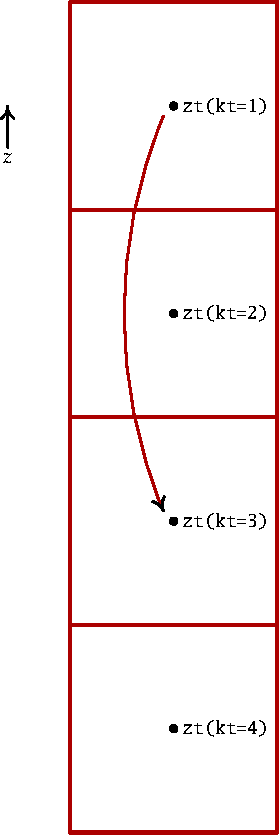
\includegraphics[angle=0,width=3cm]{./mfpic_figs/cvmix_stability_nonlocal.pdf}
\caption[Determining non-local gravitational stability]{\sf Schematic
  of the adiabatic and isohaline parcel displacement that is used to
  determine non-local gravitational stability for computing the bulk
  Richardson number according to equation
  (\ref{eq:bulk-ri-large-kpp}).  The reference temperature and
  salinity of this displaced parcel is set according to values
  determined in the surface layer, here approximated by the value at
  the top model grid cell with vertical position {\tt zt(kt=1)}.  The
  density of this parcel is then computed using the surface layer
  temperature and salinity and the local {\it in situ} pressure.  This
  displaced parcel's density is then compared to the ambient {\it in
    situ} density using the local temperature, salinity, and pressure.
  We illustrate that process by displacing the parcel to {\tt
    zt(kt=3)}.  If the resulting bulk Richardson number is larger than
  the critical value, the base of the KPP boundary layer is at or
  shallower than {\tt zt(kt=3)}, with interpolation used to determine
  the KPP boundary layer thickness $h$.  If the bulk Richarson number
  is less than the critical value, the boundary layer bottom has yet
  to be reached, so the downward search continues.}
\label{fig:cvmix_stability_nonlocal}
\end{center}
\rule{\textwidth}{0.005in}
\end{figure}
%%%%%%%%%%%%%%%%%%%%%%%%%%%%%%%%%%%%%%%%%%%%%%%%%%%%%%%%%%%%%%%%%%%%%%%%

The expression (\ref{eq:bulk-ri-large-kpp}) presents a direct means
for computing the non-local gravitational stability via the
computation of the density difference, written here using discrete
notation from Figure  \ref{fig:cvmix_stability_nonlocal}
\begin{equation}
 \delta\rho[{\tt kt},r]  = \rho[\Theta({\tt kt}), S({\tt kt}), p({\tt kt} ]  -\rho[\Theta_{r}, S_{r}, p({\tt kt})],
\label{eq:delta-density-for-nonlocal-stability}
\end{equation}
where the surface layer values $\Theta_{r}, S_{r}$ are typically
approximated by the values as {\tt kt =1}.  This approximation breaks
down for stable boundary layers with vertical grid spacing finer than
roughly 2~m, in which case an averaging is required.

There is an alternative method to approximate $\delta\rho[{\tt kt},r]$
based on linear truncations of Taylor series expansions.  The
alternative leads to a sum of squared buoyancy frequencies, analogous
to the expression
(\ref{eq:infinitesimal-delta-rho-elements-downward}).  There are some
advantages offered by the alternative approach, namely there are fewer
calculations of the equation of state, assuming we already have the
expansion coefficients $\alpha$ and $\beta$.  However, the deeper the
boundary layer, and the more nonlinear the equation of state, the less
accurate the approximation becomes.  We therefore recommend the more
exact calculation based on the density differences in equation
(\ref{eq:delta-density-for-nonlocal-stability}).

For completeness, we develop the alternative approach.  For this
purpose, consider a displacement from level {\tt kt = 1} to {\tt kt
  >1}, in which we need to compute $\rho[\Theta({\tt kt=1}),S({\tt
  kt=1}),p({\tt kt>1})]$.  Truncating a Taylor series at leading order
yields
\begin{equation}
 \rho[\Theta(1),S(1),p({\tt kt>1})]
 \approx 
 \rho[\Theta(1),S(1),p(1)] 
 - \sum\limits_{{\tt n  = 1}}^{{\tt kt}}
   {\tt dzw(n+1)} \,  \left( \frac{\partial \rho}{\partial p} \, \frac{\partial p}{\partial z}
   \right)_{ {\tt zt(n)} }.
\end{equation}
A similar expression for the {\it in situ} density $\rho[\Theta({\tt
  kt}), S({\tt kt}), p({\tt kt} ]$
\begin{equation}
 \rho[\Theta({\tt kt}),S({\tt kt}),p({\tt kt})]
 \approx 
 \rho[\Theta(1),S(1),p(1)] 
 - \sum\limits_{{\tt n  = 1}}^{{\tt kt}}
   {\tt dzw(n+1)} \,  \left( 
   \frac{\partial \rho}{\partial p} \, \frac{\partial p}{\partial z}
   + 
  \frac{\partial \rho}{\partial \Theta} \, \frac{\partial \Theta}{\partial z}
  +
  \frac{\partial \rho}{\partial S} \, \frac{\partial S}{\partial z}
   \right)_{ {\tt zt(n)} }.
\end{equation}
These results lead to the approximation 
\begin{subequations}
\begin{align}
 \delta\rho[{\tt kt},r]  &= \rho[\Theta({\tt kt}), S({\tt kt}), p({\tt kt} ]  -\rho[\Theta_{r}, S_{r}, p({\tt kt})]
 \\
 &\approx 
 -\sum\limits_{{\tt n  = 1}}^{{\tt kt}}
   {\tt dzw(n+1)} \,  \left( 
 \frac{\partial \rho}{\partial \Theta} \, \frac{\partial \Theta}{\partial z}
  +
  \frac{\partial \rho}{\partial S} \, \frac{\partial S}{\partial z}
   \right)_{ {\tt zt(n)} }
\\
 &=
 \sum\limits_{{\tt n  = 1}}^{{\tt kt}}
   {\tt dzw(n+1)} \,  \left( 
 \rho \, \alpha \, \frac{\partial \Theta}{\partial z}
  -
  \rho \, \beta \, \frac{\partial S}{\partial z}
   \right)_{ {\tt zt(n)} }
\\
 &= 
 \frac{1}{g} 
  \sum\limits_{{\tt n  = 1}}^{{\tt kt}}
   {\tt dzw(n+1)} \,  \left( \rho \, N^{2} \right)_{ {\tt zt(n)} }.
\end{align}
\label{eq:summed-n2-for-nonlocal-stability}
\end{subequations}
Again, this result is analogous to the approximate forms given in
Section \ref{subsection:buoyancy-frequency-and-stability} for the
local calculation of gravitational stability.  However, for both the
local and non-local calculation of stability, we recommend the more
exact approach that does not perform a trunction, particularly in
regions of deep mixing in the high latitudes. Making the approximation
may also compromise the ability of the KPP scheme to include
thermobaric convection.  We are thus reticent to recommend this
approach, and instead prefer the original approach given by equation
(\ref{eq:bulk-ri-large-kpp}).


\subsubsection{Unresolved velocity scale $U_{t}$ used for $\mbox{Ri}_{b}$}
\label{subsubsection:unresolved-shear}

The shear, $U_{t}/d$, in the bulk Richardson number
(\ref{eq:bulk-ri-large-kpp}) acknowledges the potential for unresolved
to impact on the boundary layer depth.  The unresolved shear acts to
deepen the boundary layer beyond that which would occur with only the
resolved shears.  \cite{LargeKPP} present an argument on their page
372 that focuses on an unresolved shear that reduces to a desired form
for the case of pure convection.  The general result is for the
velocity scale $U_{t}$ given by
\begin{subequations}
\begin{align}
 U_{t}^{2}(d) &= 
  d \, \left( \frac{C_{v} \,  (-\beta_{T})^{1/2}}{\mbox{Ri}_{c} \, \kappa^{2}} \right)
  (c_{s} \, \epsilon)^{-1/2} \, N \; w_{s}
 \\
 &= ( d \, C_{v} \, N \; w_{s} ) \, \left( \frac{ \sqrt{-\beta_{T} /  (c_{s} \, \epsilon) } }{ \, \mbox{Ri}_{c} \, \kappa^{2}} \right).
\label{eq:unresolved-shear-kpp}
\end{align}
\end{subequations}
We now summarize the terms appearing in this expression.
\begin{itemize}

\item The von Karman constant $\kappa \approx 0.40$ is chosen
  according to equation (\ref{eq:von-karman-constant}).

\item The constant $C_{v}$ sets the buoyancy frequency at the entrainment
 depth, and its value is expected to be 
\begin{equation}
 1 < C_{v} < 2. 
\label{eq:Cv-values-given-general} 
\end{equation}
 Appendix A of \cite{Dana_etal2006} provides the specific suggestion
 of 
\begin{equation}
C_{v} =  \left\{ 
\begin{array}{lc}
  2.1 - 200 \, \max(0,N)   & \qquad N \le 0.002 \, \mbox{sec}^{-1}
\\
  1.7 & \mbox{otherwise}. 
\end{array}
\right.
\label{eq:Cv-values-given} 
\end{equation}

\item The constant $c_{s}$ is part of the similarity function for
  scalar fields discussed in Section
  \ref{subsection:m-o-similarity-functions}.  It has a value $c_{s} =
  98.96$ according to equation (\ref{eq:cs-defined}).

\item The constant $\beta_{T}$ is discussed in the caption to Figure
  \ref{fig:kpp-figure1-reproduced}, and it is the ratio of the
  buoyancy flux at the entrainment depth, $h_{e}$, to the buoyancy
  flux at the surface,
\begin{equation}
 \overline{w \, b}^{d=h_{e}} = \beta_{T}   \; \overline{w \, b}^{0},
\end{equation}
 with 
\begin{equation}
 \beta_{T} \approx -0.2
\end{equation}
an empirical result.  

\item The critical Richardson number, $\mbox{Ri}_{c}$, is used to
  determine when the boundary layer base is reached, in which case
  stratification and/or reduced shear lead to a bulk Richardson number
  larger than the critical value.  \cite{LargeKPP} choose the value
\begin{equation}
 \mbox{Ri}_{c} = 0.3.  
\label{eq:large-critical-bulk-ri}
\end{equation}

\item The dimensionless number $\epsilon$ determines the thickness of
  the surface layer as in Figure
  \ref{fig:boundary-layer-schematic-kpp}, with
\begin{equation}
 \epsilon = 0.1 
\end{equation}
chosen by \cite{LargeKPP}.  

\item The MOM5 code takes the buoyancy frequency $N$ appearing in
  equations (\ref{eq:unresolved-shear-kpp}) and
  (\ref{eq:Cv-values-given}) to be the absolute value of the frequency
\begin{equation}
 N  = |N|.  
\end{equation}
However, this choice is problematic in regions of unstable buoyancy
forcing, where $N^{2} < 0$ is common.  So instead, one should take 
\begin{equation}
 N = \max(0,N),
\end{equation}
 which is how this approach was implemented in POP.  
 
\item It is notable that there are no surface gravity wave parameters in the
specification of the unresolved shear.  We have more to say on this
topic in Section \ref{section:surface-waves-and-kpp}. 

\end{itemize}


\subsubsection{An algorithm to specify the unresolved velocity scale $U_{t}$}

The unresolved velocity scale $U_{t}$ (equation
(\ref{eq:unresolved-shear-kpp})) is needed for the bulk Richardson
number in equation (\ref{eq:bulk-ri-large-kpp-large-etal-form}), with
the bulk Richardson number used to compute the boundary layer depth,
$h$.  Now the unresolved velocity $U_{t}$ requires the scalar
turbulent velocity scale $w_{s}$ (Section
\ref{subsection:vertical-velocity-scale}).  Yet the scalar velocity
scale $w_{s}$ in turn requires the boundary layer depth $h$ since
$w_{s}$ is a function of the dimensionless boundary layer depth
$\sigma = d/h$ (equation (\ref{eq:sigma-defined})). 

One method to resolve the above circular argument is to iterate.
Another means, employed by the KPP code in POP and MOM, is based on
the following observation.  Namely, to compute the boundary layer
depth $h$ we determine the depth below which the bulk Richardson
number is larger than the critical Richardson number (equation
(\ref{eq:critical-bulk-richardson-number})).  In determining that
depth, we proceed as follows for each horizontal grid point.
\begin{itemize}

\item For a grid level $k$, assume the boundary layer depth, $h$,
  equals to the depth of a tracer grid point, $d$, in which case
  $\sigma = 1$ and $h = d$.

\item Compute the turbulent velocity scale for scalars, $w_{s}$, as a
  function of the buoyancy forcing and wind forcing (Section
  \ref{subsection:vertical-velocity-scale}).

\item Compute the unresolved velocity scale $U_{t}$ (equation
  (\ref{eq:unresolved-shear-kpp})).

\item Compute the bulk Richardson number $\mbox{Ri}_{b}$ (equation
  (\ref{eq:bulk-ri-large-kpp-large-etal-form})).

\item If $\mbox{Ri}_{b} < \mbox{Ri}_{c}$, then we are still within the
  surface boundary layer, in which case the algorithm proceeds
  downward by one grid cell.

\item If $\mbox{Ri}_{b} \ge \mbox{Ri}_{c}$, then we have penetrated
  below the boundary boundary layer, in which case the algorithm
  interpolates to determine the actual boundary layer depth $h$.

\item Once the boundary layer depth is known, we compute the turbulent
  velocity scale $w_{\lambda}$, which is used to compute the KPP
  boundary layer diffusivity according to equation
  (\ref{eq:kpp-diffusivity-again}).

\end{itemize}

\subsubsection{Minimum value for the unresolved velocity scale $U_{t}$}

\color{red} This discussion needs some refinement.  \color{black} 

In the testing of the CVMix implementation of KPP in MOM6, we
considered a trivial one-dimensional situation of neutral forcing
($B_{f} = 0$) and initially uniform temperature and salinity.  We also
maintained a zero resolved velocity through use of periodic lateral
boundary conditions.  The initially uniform temperature and salinity
means that the buoyancy frequency is zero, in which case the
unresolved velocity (\ref{eq:unresolved-shear-kpp}) vanishes.  The
numerator and denominator of the bulk Richardson number thus vanish on
the first time step.  To remove the computational singularity
associated with $0/0$, we add a small positive number to the
denominator, in effect placing a minimum on the unresolved squared
velocity $U_{t}^{2}$.  This approach follows {\it Alistair Adcroft's
  Theorem}, in which division by zero in an ocean model should be
replaced by zero.  The trivial test then proceeds with nothing
happening, regardless the wind stress, which is physically what should
occur given that the buoyancy forcing vanishes and the temperature and
salinity are uniform.

Now impose a positive buoyancy forcing to the above test, again with
nonzero wind acting on a uniform initial condition for temperature and
salinity.  If strong enough, mechanical energy from the winds mixes
the positive buoyancy into the ocean over a nonzero boundary layer
region, with the boundary layer deepening as long as the mechanical
mixing is maintained.  However, in some one-dimensional tests, this
physical expectation was found to be sensitive to computational
roundoff in the calculation of the buoyancy frequency.  The resulting
boundary layer depth in turn asymptoted to a fixed value that never
deepened and was independent of the wind stress.  The upper ocean
buoyancy thus increased without bound.  

The spurious behaviour in this test is removed by enabling a
sufficiently large unresolved velocity $U_{t}^{2}$ to overcome
computational roundoff in the calculation of $N$.  Using double
precision for the computations, we have found
\begin{equation}
  \left( U_{t}^{2} \right)_{\mbox{\tiny minimum}} \approx 10^{-11}~\mbox{m}^{2}~\mbox{s}^{-2}  
\end{equation}
is sufficient to recover physically consistent behaviour for this
particular test case.  With a nontrivial denominator, the bulk
Richardson number is small in the upper ocean but large below the
boundary layer, allowing for enhanced mixing to move the positive
buoyancy into the interior, further deepening the boundary layer as
the simulation proceeds.


\subsubsection{Restrictions on $h$ under stable buoyancy forcing}

\cite{LargeKPP} suggest on page 372 that for stable buoyancy forcing,
$B_{f} > 0$, the boundary layer thickness, $h$, should be no larger
than either the Monin-Obukhov length scale, $L$, or the Ekman
length scale, 
\begin{equation}
 h_{E} = 0.7 \; u_{*} /|f|,
\label{eq:ekman-thickness}
\end{equation} 
with $f$ the Coriolis parameter.  The following reasons are noted to
motivate these two restrictions.
\begin{itemize}
\item {\sc Monin-Obukhov}: At depths deeper than $L$, buoyancy
  stratification suppresses the mechanically forced turbulence, thus
  cutting off the boundary layer.

  \item {\sc Ekman}: The Ekman depth is the extent of the boundary
    layer in neutral stratification ($N^{2} = 0$).  With stable
    buoyancy forcing, $B_{f} > 0$, we then expect the boundary layer
    depth to be less than the Ekman depth.  Note that \cite{LargeKPP}
    do not mention the origin of the $0.7$ factor in equation
    (\ref{eq:ekman-thickness}).

\end{itemize}

As noted in \cite{LargeKPP} and \cite{Large_Gent1999}, the restriction
on boundary layer thickness based on the Monin-Obukhov length has been
dropped in the NCAR implementation of KPP, as it does not lead to
favorable effects.  Dropping this constraint is also supported by the
results from \cite{Shchepetkin2005} and \cite{Lemarie_etal2012a}.
Likewise, the constraint based on the Ekman depth is not used at NCAR,
as little sensitivity was seen with its use.  Hence, there are no
restrictions for the maximum boundary layer depth under stable forcing
imposed by the NCAR implementation of KPP.  Such is the standard
approach used in the CVMix implementation.

The key problem with the Monin-Obukhov length scale, $L$, relates to
the question of how to include penetrative shortwave heating in the
calculation of the buoyancy forcing, $B_{f}$ (Section
\ref{subsection:buoyancy-forcing-obl}).  Depending on the depth over
which the penetrative heating is included (equation
(\ref{eq:penetrative-buoyancy-kpp})), one can produce a positive
Monin-Obukhov length (if including sufficient shortwave heating) or
negative (if including less heating). Since there is no fundamental
reason to choose a particular amount of the shortwave when considering
the total buoyancy forcing, there is no compelling reason to enforce
the $L$ constraint on boundary layer thickness.


\subsubsection{Noise in the boundary layer thickness}

Experience in MOM, POP, and ROMS indicate that the KPP boundary layer
thickness, $h$, can become quite noisy.  Noise in the boundary layer
thickness can translate into noise in the tracer fields within the
boundary layer.  Hence, it is common practice to apply a horizontal
smoothing operator, such as a Laplacian, to $h$ prior to its use in
computing the diffusivity or non-local transport.

The horizontal smoothing of $h$ poses an algorithmic problem for
CVMix, since CVMix modules ideally know nothing about the horizontal
grid.  There are two possible options that may be considered.
\begin{itemize}

\item {\sc intermediate $h$ sent back to calling model}: One option is
  to compute $h$ in CVMix; send it immediately back to the
  calling model for smoothing; then have the smoothed $h$ used for
  further KPP computations such as the diffusivity and non-local
  term.  

\item {\sc use previous $h$}: We compute the new value of $h$ within a
  particular call to the CMVix-KPP module, and we send this unsmoothed
  $h$ back to the calling model at the end of the CVMix-KPP module.
  But for computing the KPP diffusivities and non-local term within
  CVMix, we use the previous time step value $h$, with this earlier $h$
  having been smoothed by the calling model.  This approach requires
  storing $h$ in restart files, but that is easily handled by the
  calling model.  

\end{itemize}

This issue remains under consideration and there is no consensus
recommendation on a useful approach.


\subsection{Surface boundary condition}
\label{subsection:kpp-surface-boundary-condition}

The KPP parameterization as per \cite{LargeKPP} prescribe a vanishing
non-local flux at the ocean surface, so that
\begin{equation}
  \overline{w \, \lambda}^{\mbox{\tiny non-local}} = 0 \qquad \mbox{at $z=\eta$}.
\label{eq:non-local-surface-bc}
\end{equation}
Although standard in the KPP implementation for CVMix, we reconsider
this boundary condition in Section \ref{section:kernals-of-behaviour}
in order to remove a pathology.  For now, we note that this boundary
condition is satisfied by ensuring that the non-dimensional vertical
shape function $G_{\lambda}(\sigma)$ vanishes at $\sigma = 0$.  Since
the same shape function is used for the parameterized non-local flux
as for the diffusivity, we have
\begin{equation}
   K_{\lambda}  = 0   \qquad \mbox{at $z=\eta$}.
\end{equation}
We thus also set the local closure portion of the flux to zero at the
surface
\begin{equation}
\overline{w \, \lambda}^{\mbox{\tiny local}} = -K_{\lambda} \left( \frac{\partial \Lambda}{\partial z} \right) = 
 0  \qquad \mbox{at $z=\eta$},
\label{eq:no-flux-local}
\end{equation}

To incorporate the non-advective surface boundary fluxes (e.g.,
shortwave, longwave, latent, and sensible heat fluxes), we follow the
usual convention in which these fluxes enter as a boundary condition
on the vertical diffusion equation.  In effect we have
\begin{equation}
\overline{w \, \lambda}^{0}  = Q^{\lambda}  \qquad \mbox{at $z=\eta$}. 
\label{eq:surface-boundary-flux}
\end{equation} 
This boundary condition will be revisited in Section
\ref{section:kernals-of-behaviour}.


\subsection{Summary of the standard CVMix implementation of KPP}
\label{subsection:recommended-choices}

We summarize here the recommendations for those wishing to implement
the KPP using the CVMix code.  The main recommendation is to employ
the universal shape function (equation
(\ref{eq:universal-non-local-structure})) rather than determine this
function via the matching conditions used by \cite{LargeKPP}.
Nonetheless, the original approach is available with CVMix code, which
allows one to systematically transition to the simpler approach.

\begin{itemize}

\item The recommended parameterization of the turbulent flux is given
  by
\begin{equation}
  \overline{w \, \lambda} = -K_{\lambda} \left( \frac{\partial \Lambda}{\partial z}  \right)
   +  K_{\lambda}  \, \gamma_{\lambda}.
\label{eq:kpp-parameterization-summary}
\end{equation}
 The diffusivity is written in the form 
\begin{equation}
  K_{\lambda}(\sigma) = h \, w_{\lambda}(\sigma) \, \sigma \, (1-\sigma)^{2},
\label{eq:kpp-diffusivity-and-yet-again}
\end{equation}
where $\sigma = d/h$ is the non-dimensional boundary layer depth with
$d$ the depth, and $h$ the boundary layer thickness. We also use the
shape function
\begin{equation}
  G(\sigma)_{\mbox{\tiny universal}} = \sigma \, \ (1-\sigma)^{2}
\end{equation}
for both the local and non-local flux, and for all tracers and
momentum.

\item The vertical velocity scale, $w_{\lambda}(\sigma)$, is the same
  for each scalar tracer field, and distinct for the momentum only for
  regions of negative buoyancy flux $B_{f} < 0$.  It is proportional
  to $\kappa \, u^{*}$, where $\kappa = 0.4$ is the von Karman
  constant and $u^{*} = \sqrt{|\bftau|/\rho_{o}}$ is the friction
  velocity.  The proportionality is determined by dimensionaless
  similarity functions (Sections
  \ref{subsection:m-o-similarity-functions} and
  \ref{subsection:similarity-functions}).  These similarity functions
  are determined empirically according to analogs with the atmosphere
  as formulated within Monin-Obukov similarity theory.  This aspect of
  the KPP scheme as applied to the ocean is perhaps the least
  satisfying, since our ability to directly use atmospheric similarity
  functions for the ocean has not been tested with measurements.

\item The boundary layer depth, $h$, is determined by a bulk
  Richardson number criteria (Section
  \ref{subsection:kpp-obl-thickness}), whereby the first depth where
  $\mbox{Ri}_{b} > \mbox{Ri}_{c}$ determines the boundary layer depth.
  There are subtle issues related to the computation of the bulk
  Richardson number, with details provided in Section
  \ref{subsection:kpp-obl-thickness}.

\item The non-local flux $K_{\lambda} \, \gamma_{\lambda}$ vanishes
  for a positive surface buoyancy flux $B_{f} > 0$ and for momentum.
  For a negative surface buoyancy flux, $K_{\lambda} \,
  \gamma_{\lambda}$ provides for a vertical redistribution of surface
  tracer fluxes, so that
\begin{subequations}
\begin{align}
\overline{w \, \theta}^{\mbox{\tiny non-local}} &= K_{\theta}  \, \gamma_{\theta} = 
 - \sigma \, (1-\sigma)^{2} \, C_{s} \, \left( \frac{ Q^{\mbox{\scriptsize heat}}}{ \rho_{o}  \, C_{\mbox{\tiny p}}^{o} } \right)
\label{eq:non-local-flux-kpp-param-temp-summary}
\\
\overline{w \, s}^{\mbox{\tiny non-local}} &= K_{s}  \, \gamma_{s}  = 
 -\sigma \, (1-\sigma)^{2}  \, C_{s} \,  Q^{s}.
\label{eq:non-local-flux-kpp-param-scalar-summary}
\end{align}
\end{subequations}
The non-dimensional constant $C_{s}$ is determined according to the
similarity function for scalars, as well as other non-dimensional
coefficients (see equation (\ref{eq:cs-and-cstar-defined}).

\end{itemize}


\section{Further considerations for the KPP non-local term}
\label{section:kernals-of-behaviour}

During the testing of KPP in CVMix, we encountered some cases where
unphysical behaviour resulted.  Some of these cases were summarized
earlier, such as when motivating use of the universal shape function
$G(\sigma)$ in Section \ref{subsection:kpp-shape-function}.  We raise
further issues in this section, with particular focus on problems with
the KPP non-local flux parameterization along with potential remedies.


\subsection{KPP in the top grid cell}
\label{subsection:kpp-surface-cell-tendency}

We start our discussion by considering what happens in the $k=1$
surface model grid cell from the combined effects of surface boundary
fluxes, KPP local downgradient diffusion, and KPP non-local
redistribution of surface boundary fluxes.  We do not identify a
problem here.  Instead, our purpose is to introduce the general
behaviour that will be further explored later in this section. 
\begin{itemize}

\item {\sc convergence into top cell}: At the surface boundary,
  $z=\eta$, the parameterized local and non-local flux components
  vanish (Section \ref{subsection:kpp-surface-boundary-condition}).
  However, these flux components are nonzero at the bottom interface
  of the $k=1$ cell, with larger fluxes for thicker top grid cells.
  Hence, there is a convergence of the KPP parameterized fluxes into
  the $k=1$ cell.

\item {\sc local downgradient diffusion}: In a region stably
  stratified in temperature ($\partial \Theta / \partial z > 0$), the
  downgradient diffusive flux
\begin{equation}
\overline{w \, \theta}^{\mbox{\tiny local}} = -K_{\theta} \left( \frac{\partial \Theta}{\partial z} \right) < 0,
\end{equation}
is negative at the lower face of the $k=1$ cell.  With the no-flux
boundary condition (\ref{eq:no-flux-local}) at the ocean surface, the
parameterized local diffusive flux will cool the top model grid
cell. For $k > 1$ interior cells, the diffusive flux either cools or
warms, depending on curvature in the temperature field.

\item {\sc non-local redistibution of surface boundary flux}: The KPP
  parameterized non-local tracer flux is non-zero only for cases of
  negative buoyancy forcing.  Assuming such forcing occurs with a
  negative (cooling) surface heat flux, we already showed in Section
  \ref{subsection:kpp-surface-boundary-condition} that
  $\gamma_{\theta} > 0$ for cooling (equation
  (\ref{eq:surface-cooling-gamma-theta})).  With the no-flux surface
  boundary condition (\ref{eq:non-local-surface-bc}), we thus have a
  positive convergence of heat into the $k=1$ cell due to the KPP
  parameterized non-local flux.  Hence, the KPP non-local fluxes heat
  the $k=1$ cells whereas the parameterized downgradient diffusive
  fluxes cool this cell.

\end{itemize}

\subsection{Tracer evolution with the KPP parameterization}

We next consider effects from KPP throughout the boundary layer.  For
this purpose, return to the vertical transport equation
(\ref{eq:mean-field-equation-kpp}) and focus on the KPP parameterized
vertical processes as per the recommendations in Section
\ref{subsection:recommended-choices}.  In the presence of negative
buoyancy forcing we include the non-local KPP redistribution function,
so that evolution of an arbitrary scalar tracer (ignoring horizontal
processes) is determined by
\begin{subequations}
\begin{align}
 \frac{\partial S}{\partial t} &= 
 -\left( \frac{\partial \, (\overline{w \, s}) }{\partial z} \right) + Q^{s} \, \delta(z-\eta)
 \\
 &= 
 -\left( \frac{\partial \, (\overline{w \, s}^{\mbox{\tiny local}}) }{\partial z} \right)
 -\left( \frac{\partial \, (\overline{w \, s}^{\mbox{\tiny non-local}}) }{\partial z} \right)
 + Q^{s} \, \delta(z-\eta),
\\
 &= 
   \frac{\partial}{\partial z} \left( K \, \frac{\partial S}{\partial z} \right)
 +C_{s} \, Q^{s} \, \frac{\partial}{\partial z} [\sigma \, (1-\sigma)^{2}]
 + Q^{s} \, \delta(z-\eta)
\\
 &= 
 \underbrace{
 \frac{\partial}{\partial z} \left( K \, \frac{\partial S}{\partial z} \right)
  }_{\mbox{\tiny local downgradient diffusion}}
 - \; \; \; \underbrace{
  \left( \frac{C_{s} \, Q^{s}}{h} \right)  \, (1 - 3 \, \sigma) \, (1-\sigma)
  }_{\mbox{\tiny non-local redistribution of surface flux}} 
 \; \; \; + \underbrace{ Q^{s} \, \delta(z-\eta)}_{\mbox{\tiny surface boundary forcing}}
\label{eq:mean-field-equation-kpp-kernels}
\end{align}
\end{subequations}
where $Q^{s}$ is the surface tracer flux ($Q^{s} > 0$ means
tracer enters the ocean),
\begin{equation}
 K = h \, w \,  \sigma \, (1-\sigma)^{2}  \ge 0 
\end{equation}
is the KPP diffusivity, and we used $\sigma = (-z+\eta)/h$ so that  
\begin{equation}
 \frac{\partial \sigma}{\partial z} = -1/h.
\end{equation}
The surface boundary flux is multiplied by a Dirac delta function
(dimensions of inverse length), where
\begin{equation}
  \int\limits_{z=-h}^{z=\eta} \delta(z-\eta) \, \mathrm{d}z = 1,
\end{equation}
so that the flux appears as a surface boundary condition when
integrating the tracer budget over the surface grid cell.

To help interpret the result
(\ref{eq:mean-field-equation-kpp-kernels}), we plot the KPP structure
function $G = \sigma \, (1-\sigma)^{2}$ as well as its derivative
$G'(\sigma) = (1-3\, \sigma)(1-\sigma)$ in Figure
\ref{fig:KPP-shape-function}, from which we deduce the following
behaviours.
\begin{itemize}

\item {\sc downgradient diffusion}: The local downgradient diffusive
  portion of the KPP parameterization always acts to smooth the
  profile of a tracer, given that the diffusivity is non-negative.
  The vertical diffusivity is zero at the ocean surface, $\sigma=0$,
  and vanishes again at the boundary layer base, $\sigma=1$.  It is
  modulated by the non-dimensional shape function $G(\sigma) = \sigma
  \, (1-\sigma)^{2}$, which has a maximum at $\sigma=1/3$ (Figure
  \ref{fig:KPP-shape-function}).  In the presence of a surface
  boundary flux, vertical diffusion transports the surface flux into
  the ocean interior on a time scale set by the vertical diffusivity
  $K$ and curvature in the tracer field.

\item {\sc non-local redistribution}: The non-local portion of the KPP
  parameterization redistributes the surface flux throughout the
  boundary layer.  Its vertical structure is provided exclusively by
  the non-dimensional shape function $G(\sigma)$.  There is no
  time scale for impacts from the non-local redistribution to affect a
  point within the boundary layer. Instead, the impacts are
  instantaneous.  In the upper portion of the boundary layer, where
  $\sigma < 1/3$, the tracer tendency has a contribution that is
  opposite in sign to the surface boundary flux.  It is furthermore in
  this shallow region where the non-local parameterization has its
  largest contribution at a single grid point (Figure
  \ref{fig:KPP-shape-function}).  In constrast, for deeper reaches
  of the boundary layer with $\sigma > 1/3$, the tracer tendency has a
  contribution that has the same sign as the surface flux.

\end{itemize}



%%%%%%%%%%%%%%%%%%%% %%%%%%%%%%%%%%%%%%%%%%%%%
\begin{figure}[h!t]
\rule{\textwidth}{0.005in}
\begin{center}
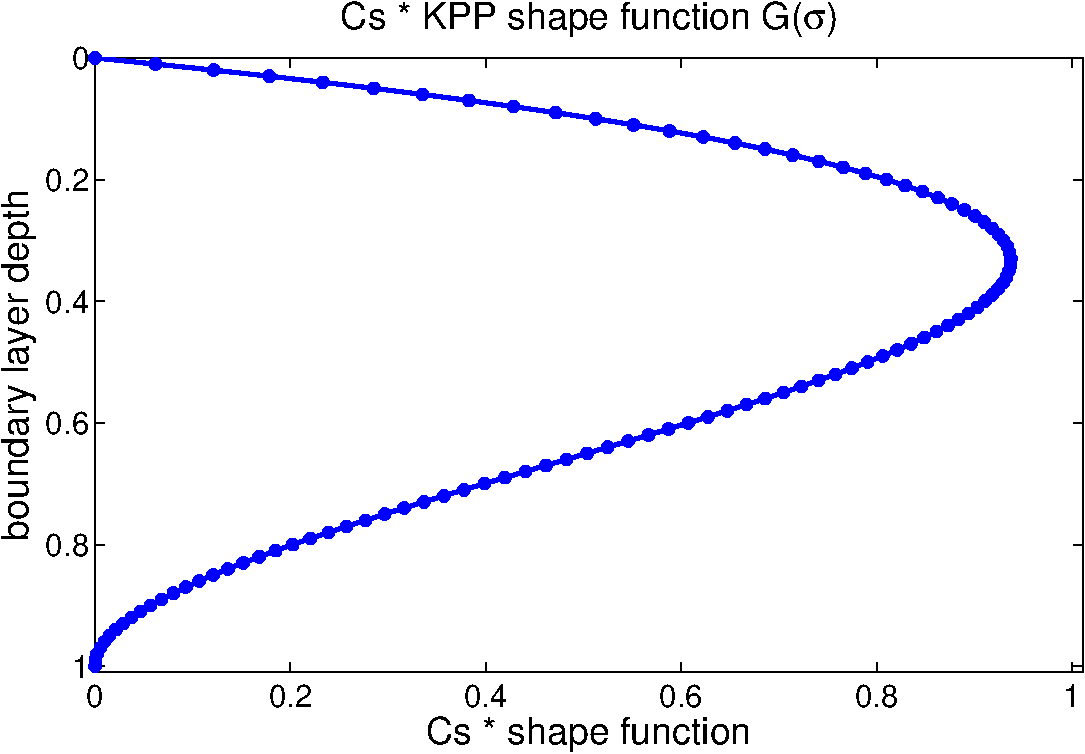
\includegraphics[angle=0,width=7cm]{./figs/KPP_Gfunction.pdf}
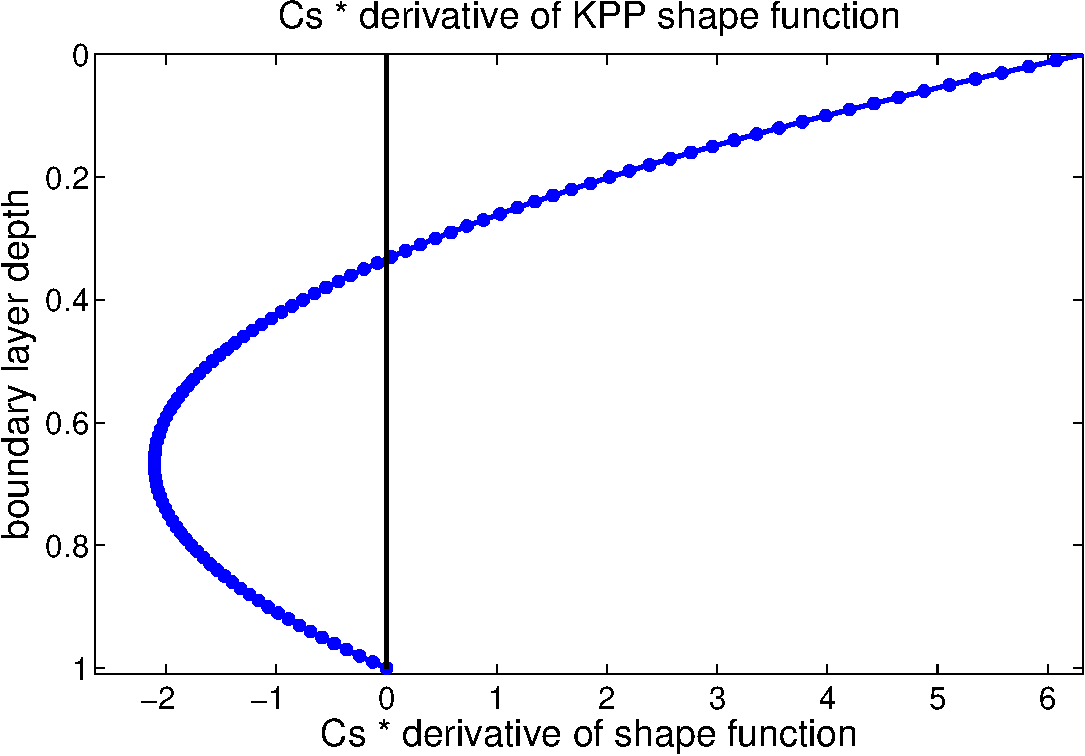
\includegraphics[angle=0,width=7cm]{./figs/KPP_Gprime.pdf}
\caption[KPP shape function]{\sf KPP shape function $G = \sigma \,
  (1-\sigma)^{2}$ multiplied by the constant $C_{s} = 6.33$ (equation
  (\ref{eq:Cs-value})) as well as its derivative $C_{s} \; G'(\sigma)
  = C_{s} \, (1-3\, \sigma)(1-\sigma)$. In the upper portion of the
  boundary layer where $\sigma < 1/3$, the derivative is positive, in
  which case the non-local contribution to KPP adds a tendency to
  tracers with a sign opposite to that of the surface boundary flux
  (see equation (\ref{eq:mean-field-equation-kpp-kernels})).  In the
  regions where $1/3 < \sigma < 1$, the KPP non-local tendency has the
  same sign as the surface boundary flux.  The largest magnitude of
  $G'(\sigma)$ is at $\sigma=0$, so that the largest impact at a
  single depth from the non-local flux convergence is in the upper
  portion of the boundary layer.  The area encompassed by $G'(\sigma)$
  in the shallow region $\sigma < 1/3$ is the same as that in the
  deeper region $1 < \sigma < 1/3$.}
\label{fig:KPP-shape-function}
\end{center}
\rule{\textwidth}{0.005in}
\end{figure}
%%%%%%%%%%%%%%%%%%%%%%%%%%%%%%%%%%%%%%%%%%%%%%%%%%%%%%%%%%%%%%%%%%%%%%%%


\subsection{A thought experiment with surface cooling}

We introduce a thought experiment to illustrate the potential for
unphysical behaviour from the KPP parameterization, in particular from
the parameterization of non-local transport of surface fluxes into the
boundary layer.  Consider constant surface cooling from sensible heat
applied to an ocean that is stratified in salinity but unstratified in
temperature, and ignore the impacts from penetrative shortwave
radiation.  There is no baroclinicity and surface forcing introduces
no resolved vertical shear.  Furthermore, assume zero surface water
fluxes.  Surface cooling thus imparts a negative buoyancy forcing,
which means the KPP non-local redistribution function is
active. Surface winds blow, but they are not fundamental to our
considerations.

The tracer equation (\ref{eq:mean-field-equation-kpp-kernels}) for
temperature takes the form
\begin{equation}
 \frac{\partial \Theta}{\partial t} = 
   \frac{\partial}{\partial z} \left( K \, \frac{\partial \Theta}{\partial z} \right)
 - |Q_{\theta}| \left( \delta(z-\eta) - \frac{C_{s}}{h} \, (1-3 \, \sigma) \, (1-\sigma) \right).
\end{equation}
Here are the basics of the temperature evolution.
\begin{itemize}

\item Boundary layer mixing penetrates to a depth determined initially
  by the salinity stratification, but over time the developing
  temperature structure also impacts on the boundary layer depth. 

\item The local portion of KPP diffusively spreads the surface
  cooling, $Q_{\theta} < 0$, into the ocean boundary layer as the
  boundary layer deepens.

\item The KPP non-local redistribution warms the shallow regions of
  the boundary layer where $\sigma < 1/3$.  Consequently, the KPP
  non-local flux partially counteracts cooling from the downgradient
  diffusion.  Conversely, in the deeper portion of the boundary layer,
  where $\sigma > 1/3$, the non-local KPP flux enhances cooling.  For
  the full boundary layer, the KPP non-local flux acts to restratify.
  Indeed, in cases where the non-local term dominates over the local
  diffusion, these stabilizing effects can reduce, rather than
  increase, the boundary layer depth.  Conversely, for weakly
  stratified regions below the boundary layer, the introduction of
  cooling to the deeper boundary layer can destabilize the lower
  portion of the boundary layer, thus deepening the boundary layer.

\end{itemize}

As noted above, the KPP non-local term acts to increase the
temperature in the shallow portion of the boundary layer where $0 <
\sigma < 1/3$ (Figure \ref{fig:KPP-shape-function}).  We further
explore this process by considering the boundary layer at an early
time in the simulation prior to local effects from downgradient
diffusion having reached the depth considered, so that $\partial
\Theta / \partial z = 0$.  Even though diffusion has yet to reach this
depth, the instantaneous effects from convergence of the KPP non-local
flux acts to warm depths with $\sigma < 1/3$.  We thus have ocean
warming in the presence of surface cooling.  As the simulation
evolves, vertical diffusion spreads effects from surface cooling
deeper into the boundary layer, and this cooling can overcome the
warming effects from the non-local flux.  We thus tend to see the
warming from the KPP non-local flux early during a transient response
to surface cooling.

This thought experiment has been realized in various idealized
configurations of the KPP scheme using the CVMix code. We illustrate a
particular case in Figure \ref{fig:KPP_temperature_test}, with the
figure caption providing experimental details.  As seen in this
figure, the warming manifests more prominently upon refining the
vertical grid spacing.  Doing so provides more grid points within the
upper portion of the boundary layer, where the vertical diffusion
effects are dominated by the non-local term.  With a coarse enough
vertical grid, evidence of spurious warming disappears.

In addition to noting problems with warming depths in the presence of
surface cooling, it is trivial to illustrate problems in the case of
an initially uniform passive tracer with a nonzero surface flux that
adds tracer to the ocean.  A negative passive tracer concentration
arises during the early portion of the simulation, again due to the
convergence of the KPP non-local flux in the region $\sigma < 1/3$.

In realistic configurations, time evolution of scalar fields may be
dominated by effects such as advection and lateral mixing in a way
that hides unphysical behaviour from the non-local KPP
parameterization.  Furthermore, the unphysical effects identified here
occur in transient situations. Studies such as \cite{LargeKPP} focused
instead on the steady state.  Our results motivate investigating
alternatives to the shape function used for the parameterized
non-local flux, particularly in order to properly represent the
transient behaviour.


%%%%%%%%%%%%%%%%%%%% %%%%%%%%%%%%%%%%%%%%%%%%%
\begin{figure}[h!t]
\rule{\textwidth}{0.005in}
\begin{center}
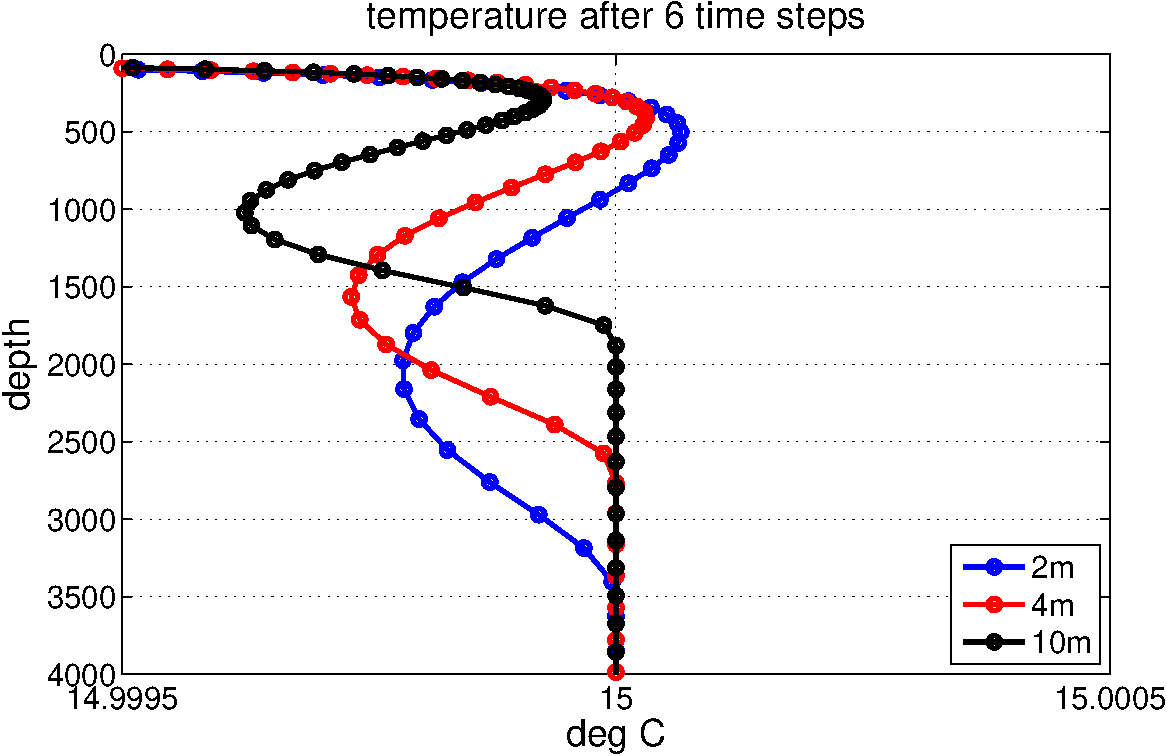
\includegraphics[angle=0,width=10cm]{./figs/KPP_temperature_test.pdf}
\caption[KPP temperature test]{\sf Temperature profiles after six time
  steps (each of one hour) for three different model grids from an
  idealized one-dimensional simulation.  Each grid has 75 levels down
  to 6000~m (upper 4000~m shown here), with the upper ocean spacing
  noted in the figure. The simulation is forced with
  $-100~\mbox{W}~\mbox{m}^{-2}$ sensible heat flux, and no penetrative
  radiation.  The temperature profile is initially uniform at
  $15^{\circ}C$, whereas the salinity profile is stable with the
  surface value of $35$ and bottom value of $35.01$.  The equation of
  state is linear, with $\rho = \rho_{o} \, (1 - \alpha \, \Theta +
  \beta \, S)$, where $\alpha = 2.55 \, \times \,
  10^{-4}\mbox{}^{\circ}C^{-1}$, and $\beta = 7.4 \, \times \,
  10^{-4}\mbox{ppt}^{-1}$.  Winds are applied with a stress of
  $0.1~\mbox{N}~\mbox{m}^{-2}$.  The domain is periodic and there are
  no horizontal gradients, so that no resolved shear contributes to
  the bulk Richardson number calculation.  Regions with temperatures
  larger than the initial uniform $15^{\circ}C$ are unphysical, since
  they appear even though the surface is being cooled.  Spurious
  warming is more prominent in the fine resolution simulation (2~m),
  whereas the coarse spaced grid (10~m) shows no sign of spurious
  warming due to the relatively larger contribution from vertical
  diffusion.}
\label{fig:KPP_temperature_test}
\end{center}
\rule{\textwidth}{0.005in}
\end{figure}
%%%%%%%%%%%%%%%%%%%%%%%%%%%%%%%%%%%%%%%%%%%%%%%%%%%%%%%%%%%%%%%%%%%%%%%%


\subsection{Modified shape function for the KPP non-local flux}
\label{subsection:modified-kpp-structure}

In so far as properly representing the transient behaviour to a
negative surface buoyancy flux, we identify the following two problems
with the KPP non-local redistribution as parameterized by the
shape function $G(\sigma) = \sigma \, (1-\sigma)^{2}$.

\begin{itemize}

\item It redistributes a surface flux into the shallow boundary layer
  region ($\sigma < 1/3$) with an opposite sign to the surface flux
  itself.

\item It affects the boundary layer instantaneously. 

\end{itemize}
Unsatisfying elements from the instantaneous impacts become
increasingly apparent when considering refined resolution models.
Model time steps of a few minutes mean that the full extent of a
boundary layer is impacted within minutes by changes in surface
fluxes.  This very short response time is reminiscient of the full
convection parameterizations of the 1990s (e.g.,
\cite{Rahmstorf1993}), which have largely been displaced by diffusive
adjustment schemes that allow for a nonzero time scale (e.g.,
\cite{KlingerConvection}).  Nonetheless, within the framework of the
KPP parameterization of non-local fluxes, we see no alternative to the
instantaneous response.

However, we do see alternatives to the shape function used for the
parameterized non-local flux.  We denote this new function by
$\mathcal{G}(\sigma)$ to distinguish it from $G(\sigma)$ used for the
diffusivity.  We emphasize that our considerations leave untouched the
shape function for the diffusivity, which still takes the form
$G(\sigma) = \sigma \, (1-\sigma)^{2}$.  Contrary to the $G(\sigma)$
shapee function, we insist that $\mathcal{G}(\sigma)$ be monotonic,
thus eliminating the sign change that causes problems with use of
$G(\sigma)$ for the parameterized non-local flux.  We also wish to
maintain a shape function that vanishes at the bottom of the boundary
layer, so that
\begin{equation}
  \mathcal{G}(\sigma = 1)   = 0.
\end{equation}

Given this lower boundary condition, a nontrivial shape function must
have a nonzero surface value.  Having $\mathcal{G}(0) \ne 0$ is
fundamentally distinct from the constraint $G(0) = 0$ imposed by
\cite{LargeKPP}.  However, having a non-zero non-local flux at the
ocean surface may in fact be physically appropriate.  Namely, we
consider the non-local flux to be a redistribution of the surface flux
into the boundary layer.  Consequently, we may choose to let the
parameterized non-local flux equal to the surface boundary flux when
approaching the ocean surface, $\sigma \rightarrow 0$.  That is,
\begin{subequations}
\begin{align}
  \overline{w \, s}^{\mbox{\tiny non-local}} (\sigma=0) &= -Q^{s}   
 \\
  &= -C_{s} \, \mathcal{G}(0)\, Q^{s} 
 \\
 & \Rightarrow  \mathcal{G}(0) = C_{s}^{-1},
\end{align}
\end{subequations}
where the minus sign in the first equation arose from the sign
convention whereby $\overline{w \, s}^{\mbox{\tiny non-local}} > 0$
implies tracer leaving the ocean, whereas $Q^{s} > 0$ signals tracer
entering the ocean (see Section \ref{subsection:conventions}).  

Given the above considerations, we have investigated the following
three shape functions
\begin{subequations}
\begin{align}
 C_{s} \,  \mathcal{G}(\sigma) &= 1 - \sigma 
\label{eq:non-local-shape-function-linear}
 \\
 C_{s} \,  \mathcal{G}(\sigma) &= (1 - \sigma)^{2}
\label{eq:non-local-shape-function-parabolic}
 \\
 C_{s} \,  \mathcal{G}(\sigma) &= 1 + (2 \, \sigma  - 3) \, \sigma^{2}.
\label{eq:non-local-shape-function-cubic}
\end{align}
\end{subequations}
The linear function has a constant nonzero slope, whereas the
parabolic and cubic functions satisfy $\mathcal{G}'(\sigma = 1) = 0$.
In Figure \ref{fig:KPPmod-shape-function} we plot the three
modified shape functions and their derivatives.  The non-local flux is
parameterized by (compare to equation
(\ref{eq:non-local-flux-kpp-param-scalar-summary}))
\begin{equation}
 \overline{w \, s}^{\mbox{\tiny non-local}} = - C_{s} \, \mathcal{G} \, Q^{s} 
\label{eq:non-local-flux-kpp-param-scalar-new-form}
\end{equation}
and its vertical convergence, which determines the tracer tendency,
takes the form
\begin{subequations}
\begin{align}
 -\frac{\partial}{\partial z} \left( \overline{w \, s}^{\mbox{\tiny non-local}} \right)_{\mbox{\tiny linear}} 
 &= \left( \frac{Q^{s}}{h} \right)
 \\
-\frac{\partial}{\partial z} \left( \overline{w \, s}^{\mbox{\tiny non-local}} \right)_{\mbox{\tiny parabolic}} 
 &= \left( \frac{2 \, Q^{s}}{h} \right) (1-\sigma)
 \\
-\frac{\partial}{\partial z} \left( \overline{w \, s}^{\mbox{\tiny non-local}} \right)_{\mbox{\tiny cubic}} 
 &= \left( \frac{6 \, Q^{s}}{h} \right) \sigma \, (1-\sigma).
\end{align}
\end{subequations}
The resulting tracer tendency
(\ref{eq:mean-field-equation-kpp-kernels}) is given by 
\begin{subequations}
\begin{align}
 \left( \frac{\partial S}{\partial t} \right)_{\mbox{\tiny linear}} &= 
 \underbrace{
 \frac{\partial}{\partial z} \left( K \, \frac{\partial S}{\partial z} \right)
  }_{\mbox{\tiny local downgradient diffusion}}
 + \; \; \underbrace{
  \left( \frac{Q^{s}}{h} \right)
  }_{\mbox{\tiny non-local redistribution}} 
\label{eq:mean-field-equation-kpp-kernels-modified-linear}
\\
 \left( \frac{\partial S}{\partial t} \right)_{\mbox{\tiny parabolic}} &= 
 \underbrace{
 \frac{\partial}{\partial z} \left( K \, \frac{\partial S}{\partial z} \right)
  }_{\mbox{\tiny local downgradient diffusion}}
 + \; \; \underbrace{
  \left( \frac{2 \, Q^{s}}{h} \right)  \, (1-\sigma)
  }_{\mbox{\tiny non-local redistribution}} 
\label{eq:mean-field-equation-kpp-kernels-modified-parabolic}
\\
 \left( \frac{\partial S}{\partial t} \right)_{\mbox{\tiny cubic}} &= 
 \underbrace{
 \frac{\partial}{\partial z} \left( K \, \frac{\partial S}{\partial z} \right)
  }_{\mbox{\tiny local downgradient diffusion}}
 + \; \; \underbrace{
  \left( \frac{6 \, Q^{s}}{h} \right)  \, \sigma \, (1-\sigma),
  }_{\mbox{\tiny non-local redistribution}} 
\label{eq:mean-field-equation-kpp-kernels-modified-cubic}
\end{align}
\end{subequations}
in which we see that the non-local redistribution retains the sign of
the surface flux throughout the boundary layer where $0 \le \sigma \le
1$.  Note that the delta-function distributed surface flux, present in
the formulation (\ref{eq:mean-field-equation-kpp-kernels}), has been
dropped from equations
(\ref{eq:mean-field-equation-kpp-kernels-modified-linear})--(\ref{eq:mean-field-equation-kpp-kernels-modified-cubic}).
The reason is that the surface boundary condition has been absorbed by
the parameterized non-local flux.  That is, the boundary condition
(\ref{eq:surface-boundary-flux}) is now directly part of the
parameterized flux.  Nonetheless, the reformulation of the boundary
condition for the parameterized non-local flux leads to no code
changes, since the boundary flux is introduced to the ocean in the
same manner regardless the shape function.


%%%%%%%%%%%%%%%%%%%% %%%%%%%%%%%%%%%%%%%%%%%%%
\begin{figure}[h!t]
\rule{\textwidth}{0.005in}
\begin{center}
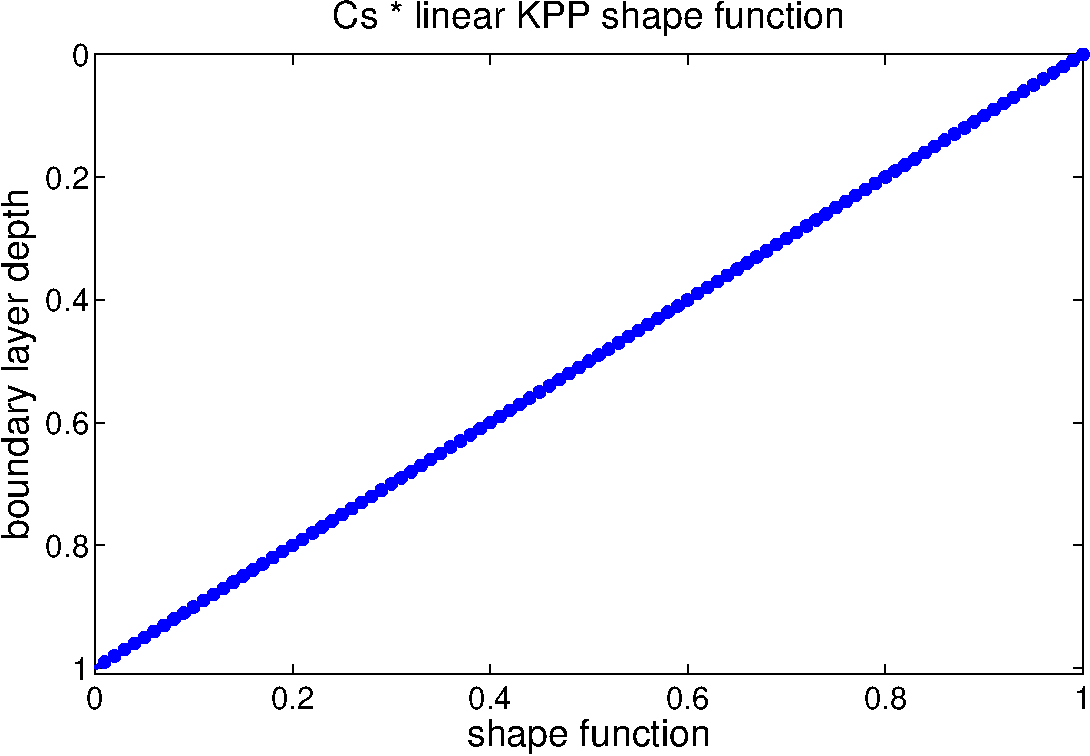
\includegraphics[angle=0,width=5cm]{./figs/KPPmod_linear_Gfunction.pdf}
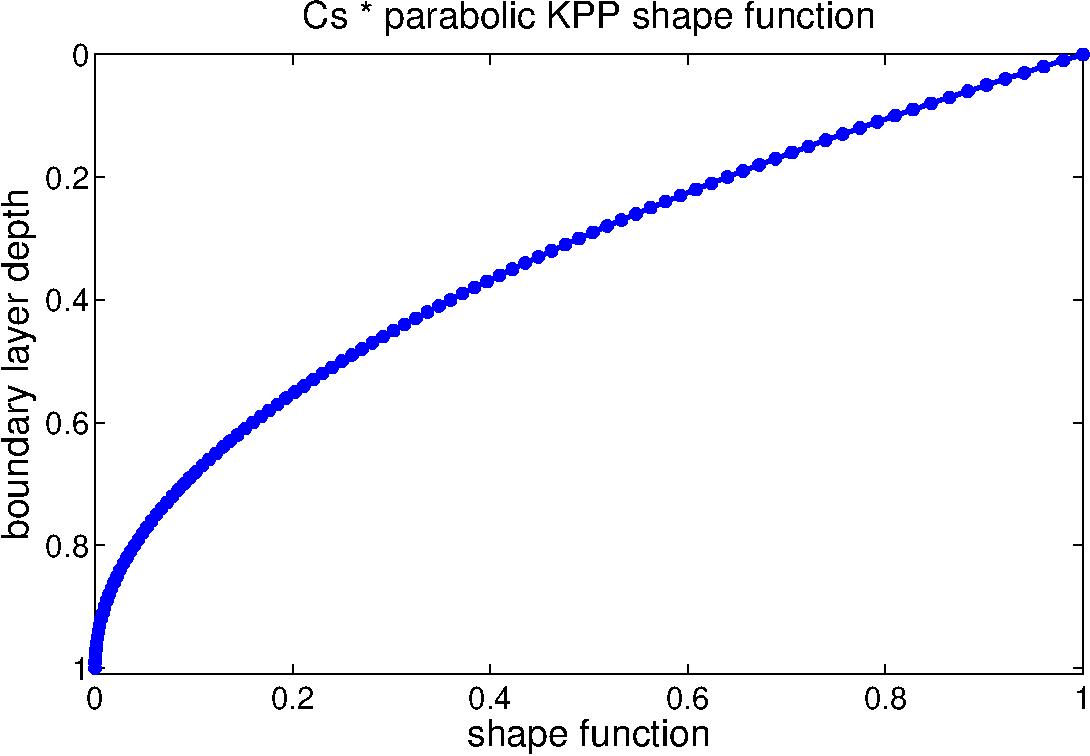
\includegraphics[angle=0,width=5cm]{./figs/KPPmod_parabolic_Gfunction.pdf}
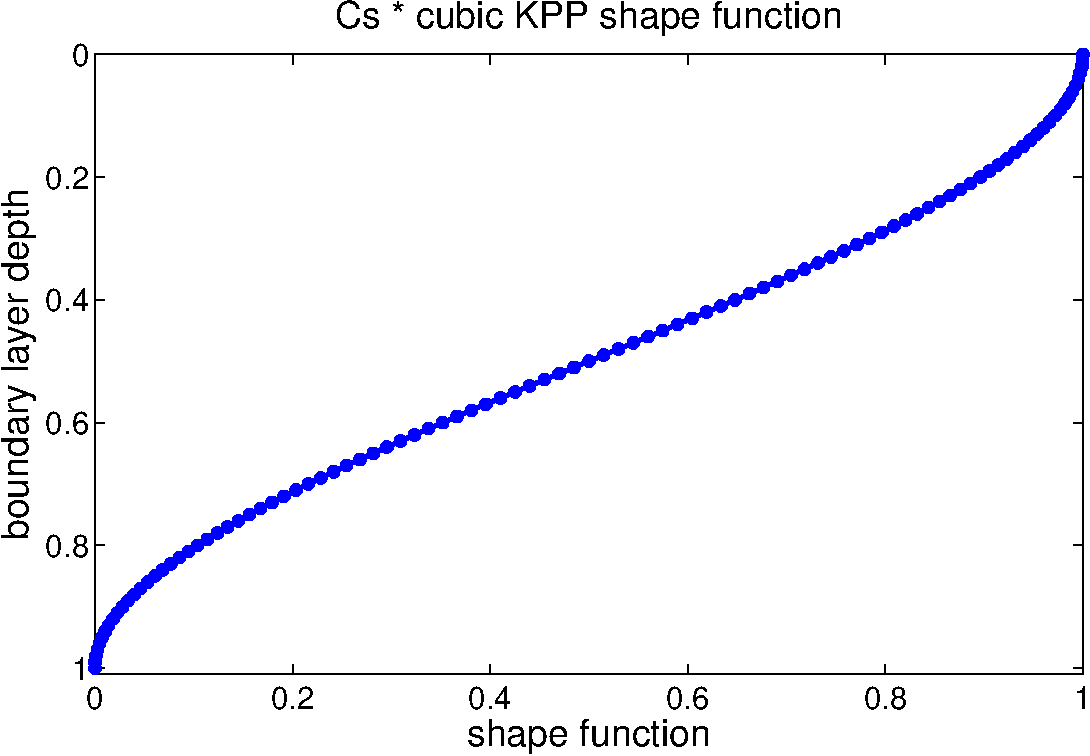
\includegraphics[angle=0,width=5cm]{./figs/KPPmod_cubic_Gfunction.pdf}
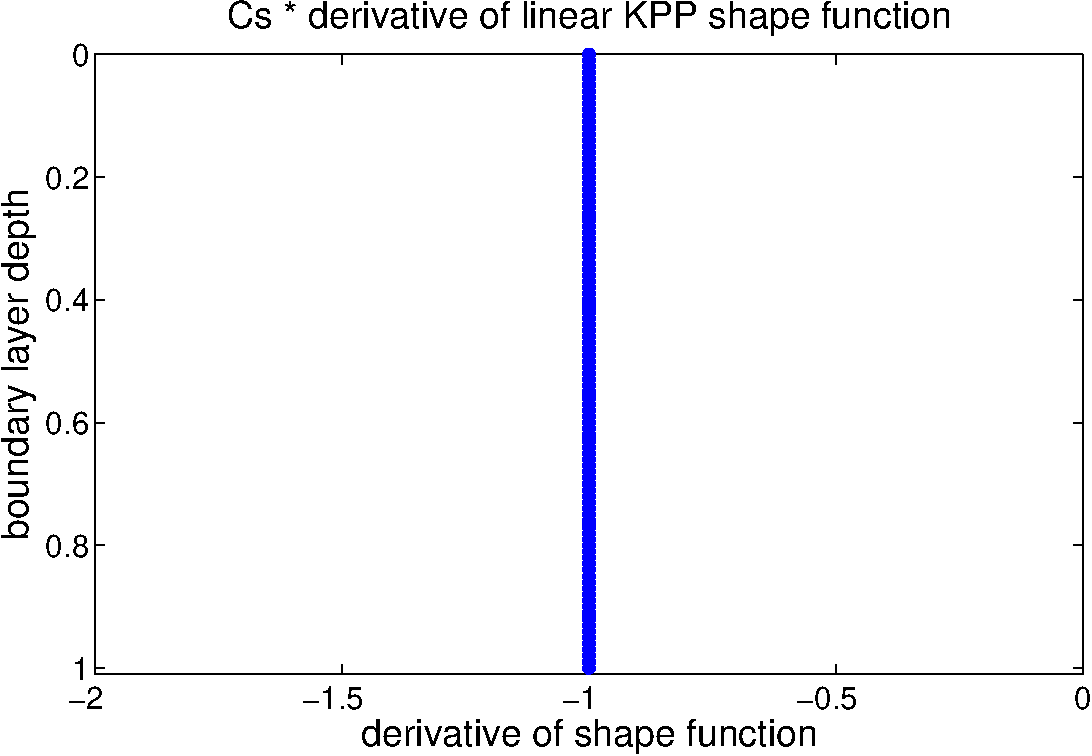
\includegraphics[angle=0,width=5cm]{./figs/KPPmod_linear_Gprime.pdf}
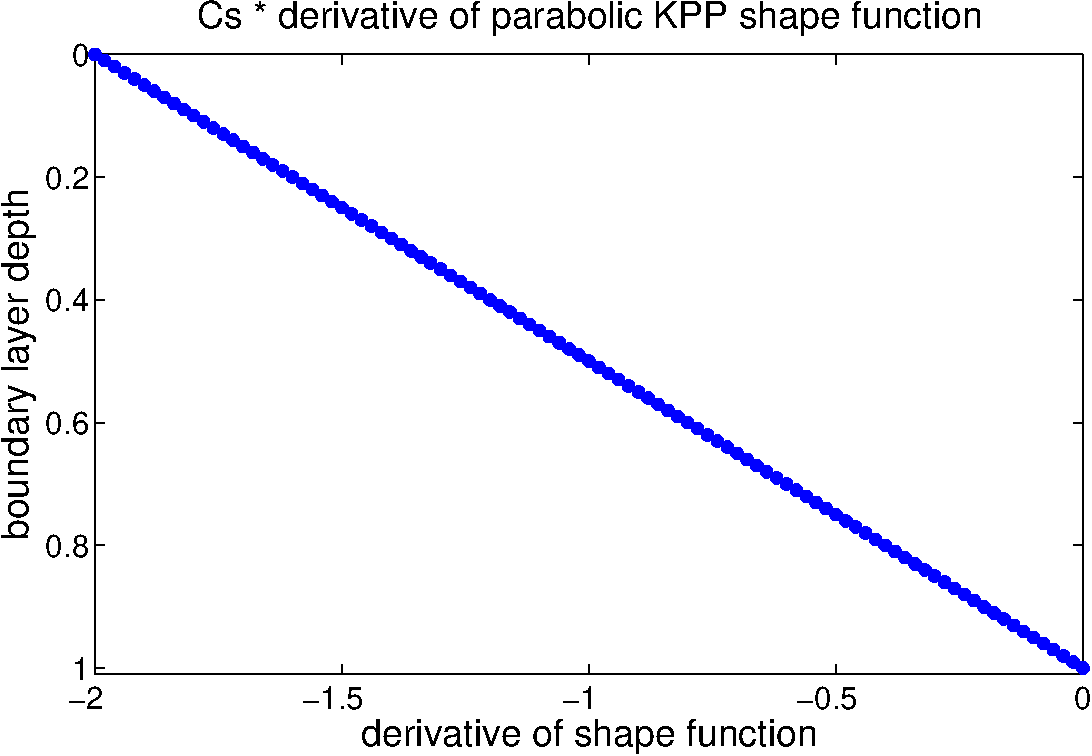
\includegraphics[angle=0,width=5cm]{./figs/KPPmod_parabolic_Gprime.pdf}
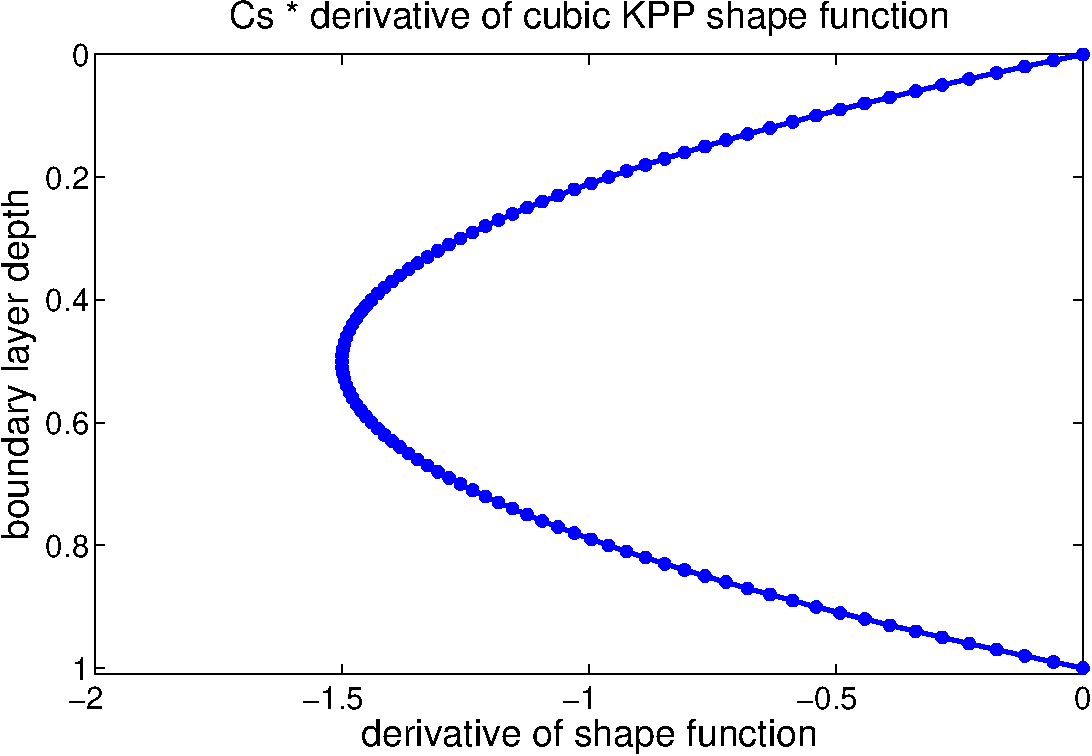
\includegraphics[angle=0,width=5cm]{./figs/KPPmod_cubic_Gprime.pdf}
\caption[Modified KPP shape function]{\sf Modified KPP shape functions
  according to equations
  (\ref{eq:non-local-shape-function-linear})--(\ref{eq:non-local-shape-function-cubic}):
  linear function $C_{s} \, \mathcal{G}(\sigma) = 1 - \sigma$;
  parabolic function $C_{s} \, \mathcal{G}(\sigma) = (1 -
  \sigma)^{2}$; and cubic function $C_{s} \, \mathcal{G}(\sigma) = 1 +
  (2 \, \sigma - 3) \, \sigma^{2}$.  Also shown are their derivatives:
  linear function $C_{s} \, \mathcal{G}'(\sigma) = -1$; parabolic
  function $C_{s} \, \mathcal{G}'(\sigma) = -2 \, (1 - \sigma)$; and
  cubic function $C_{s} \, \mathcal{G}'(\sigma) = -6 \, \sigma \, (1-
  \sigma)$.  Note the monotonic nature of the function, which has a
  linear derivative of one sign throughout the boundary layer where $0
  \le< \sigma \le 1$.}
\label{fig:KPPmod-shape-function}
\end{center}
\rule{\textwidth}{0.005in}
\end{figure}
%%%%%%%%%%%%%%%%%%%%%%%%%%%%%%%%%%%%%%%%%%%%%%%%%%%%%%%%%%%%%%%%%%%%%%%%


\subsection{Tests with the modified KPP non-local shape function}
\label{subsection:tests-of-kpp-modified-non-local}

Figure \ref{fig:non-local-shape-compare} shows results from the
modified shape functions
(\ref{eq:non-local-shape-function-linear})--(\ref{eq:non-local-shape-function-cubic})
in the idealized test described in Figure
\ref{fig:KPP_temperature_test}.  The first panel shows the very small
sensivity to vertical grid spacing when using the parabolic function
(equation (\ref{eq:non-local-shape-function-parabolic})).  This small
sensitivity contrasts to the results from the original shape function
as shown in Figure \ref{fig:KPP_temperature_test}.  All three of the
new shape functions show similar small sensitivity to the vertical
grid.  Furthermore, there is no sign of spurious warming with the new
functions.

The second panel in Figure \ref{fig:non-local-shape-compare} exhibits
sensitivity to the use of the linear, parabolic, or cubic shape
functions
(\ref{eq:non-local-shape-function-linear})--(\ref{eq:non-local-shape-function-cubic}).
The parabolic shape function generally renders a deeper boundary
layer.  We can understand that effect by noting that the parabolic
shape function places the largest amount of cooling into the upper
ocean, as revealed by the derivative shown in Figure
\ref{fig:KPPmod-shape-function}.  It is unclear how general this
result is, though note that preliminary results from a more realistic
seasonally forced test case that also show deeper boundary layers with
the parobolic shape function.

%%%%%%%%%%%%%%%%%%%% %%%%%%%%%%%%%%%%%%%%%%%%%
\begin{figure}[h!t]
\rule{\textwidth}{0.005in}
\begin{center}
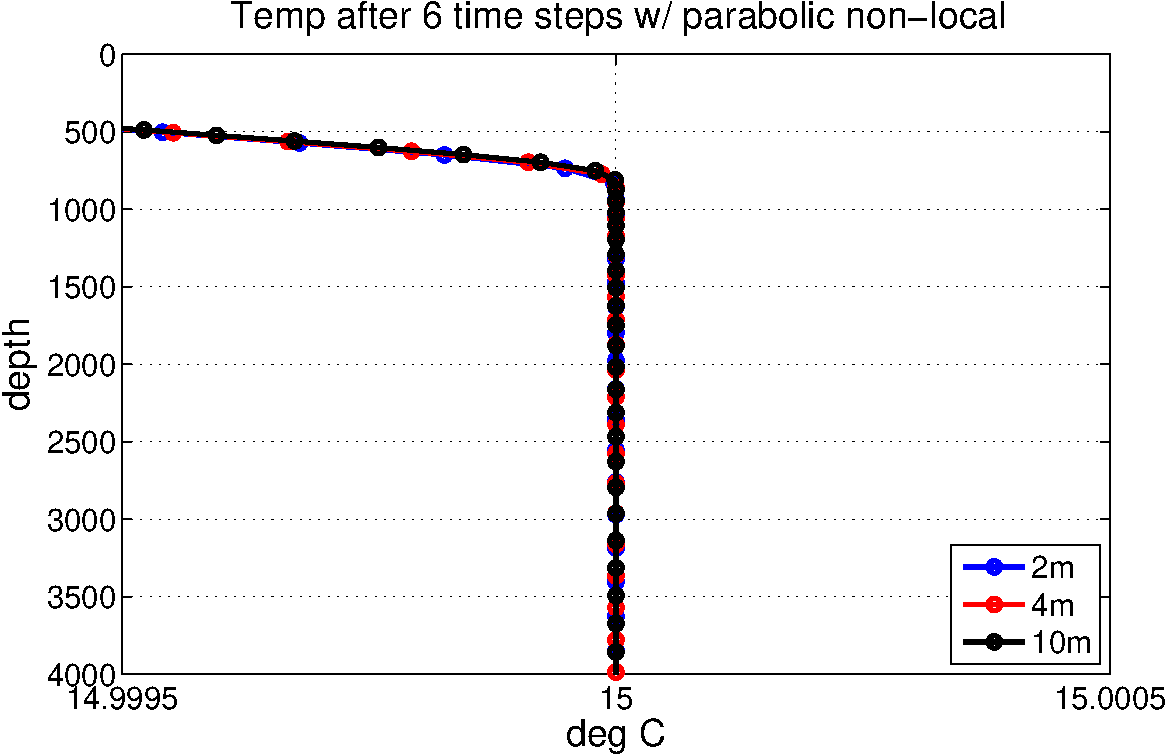
\includegraphics[angle=0,width=8cm]{./figs/KPP_temperature_parabolic_nonlocal.pdf}
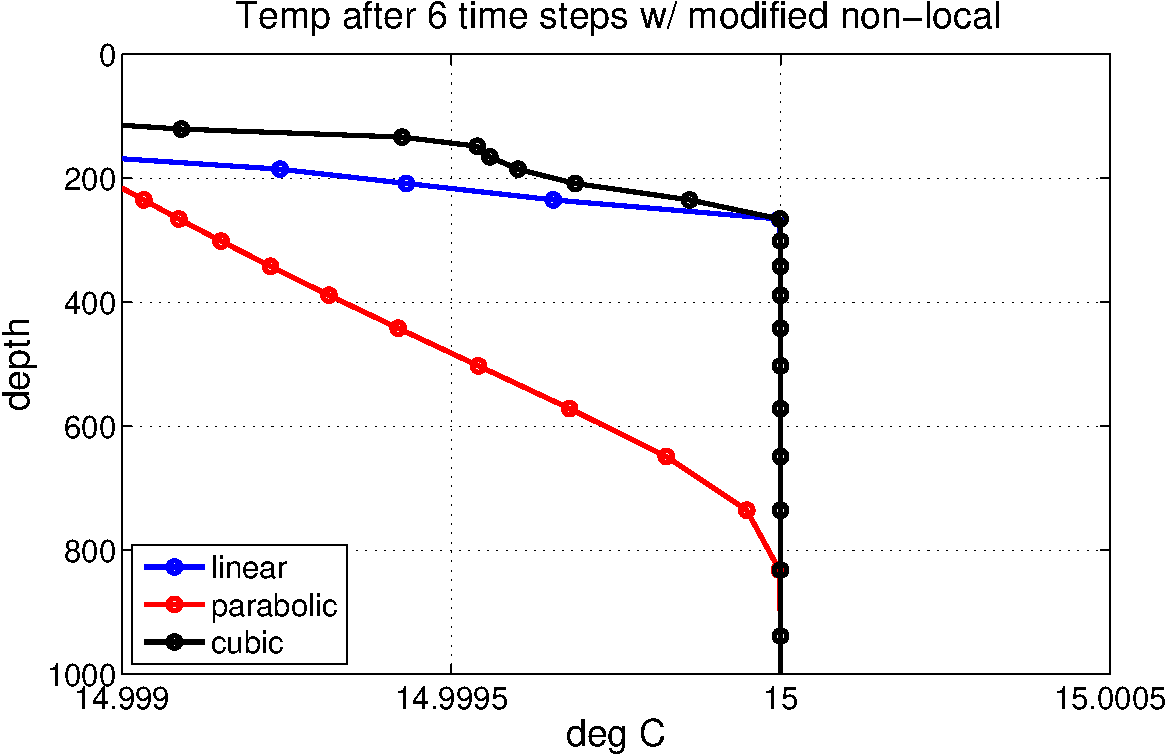
\includegraphics[angle=0,width=8cm]{./figs/KPP_temperature_linear_para_cubic_nonlocal.pdf}
\caption[KPP temperature test with modified non-local]{\sf Temperature
  profiles after six time steps (each of one hour).  The first panel
  shows sensitivity to three different model grids from an idealized
  one-dimensional simulation using the parabolic shape function
  $\mathcal{G} = (1-\sigma)^{2}$ (equation
  (\ref{eq:non-local-shape-function-parabolic})) for the parameterized
  non-local flux.  Details of the grid and experimental design are
  given in the caption to Figure \ref{fig:KPP_temperature_test}.  Note
  the absence of any water warmer than $15^{\circ}C$, and the close
  agreement for the three simulations with different vertical grid
  spacings.  These results contrast with those shown in Figure
  \ref{fig:KPP_temperature_test} realized with the shape function $G =
  \sigma \, (1-\sigma)^{2}.$ The second panel here shows sensitivity
  to the modified non-local structure functions. The parabolic
  function exhibits the deeper boundary layer relative to the linear
  and cubic functions.  Note the different horizontal and vertical
  scales for the two panels.}
\label{fig:non-local-shape-compare}
\end{center}
\rule{\textwidth}{0.005in}
\end{figure}
%%%%%%%%%%%%%%%%%%%%%%%%%%%%%%%%%%%%%%%%%%%%%%%%%%%%%%%%%%%%%%%%%%%%%%%%



\section{KPP with surface waves}
\label{section:surface-waves-and-kpp}

\cite{Craig_Banner_1994} considered surface waves in a modification of
the \cite{MellorYamada1982} 2.5 order turbulence scheme.
\cite{Axell_2002} considered also Langmuir turbulence in the
$k-\epsilon$ closure scheme.  We consider here some issues related to
introducing both waves and Langmuir turbulence in the KPP scheme.

The KPP formulation presented by \cite{LargeKPP} ignores surface waves
and the associated breaking waves and Langmuir turbulence.  The basis
for KPP must be revisited in regions of waves, since waves modify the
Monin-Obukhov similarity scalings (see \cite{Terray_etal1996} for the
case of breaking waves, and Section 2.2 of
\cite{SullivanMcWilliams2010} for wave-driven winds).  In the presence
of waves, the ocean surface contains both breaking waves to enhance
upper ocean mixing and dissipation; swell, which can modify the the
atmospheric planetary boundary layer by providing momentum to lower
atmospheric winds; and the coupling of Stokes drift to currents to
produce Langmuir cells and associated turbulence
\citep{McWilliams_etal1997}.  These processes act in addition to and
in interaction with the shear induced eddies and buoyant plumes
traditionally considered as part of the KPP scheme.  The modifications
to KPP with waves represents a research project, with work from
\cite{Belcher_etal2012} a step towards this goal, in which they
consider the regimes where winds are more or less important than
Langmuir turbulence.

In this section, we identify some incremental steps that may be
considered for modifying aspects of KPP to incorporate features of
surface waves.  Even with these more humble aspirations, there are
many questions.


\subsection{Modified budgets with Stokes velocity}
\label{subsection:stokes-into-pe-kpp}

Large eddy simulations that incorporate surface waves, such as those
from \cite{McWilliamsSullivanMoeng1997}, \cite{McWilliamsSullivan2001}
and \cite{SullivanMcWilliams07}, include a contribution in the
momentum equation from the Stokes velocity on the Coriolis force as
well as a vortex force.  Additionally, the tracer equation includes
advection from the Stokes velocity.  Finally, the subgrid scale
turbulent kinetic energy equation also includes advection by the
Stokes velocity, as well as vertical shear of the Stokes velocity
coupled to the subgrid scale stresses, thus acting as a source for
turbulent kinetic energy. Mathematically, these terms take the form
(see equations (4a), (4b) and (4c) from \cite{SullivanMcWilliams2010})
\begin{align}
\frac{\partial {\bf v}}{\partial t} &= \ldots -f \, \hat{\bf z} \, \wedge \, {\bf v}^{\mbox{\tiny stokes}}  
 + {\bf v}^{\mbox{\tiny stokes}}  \, \wedge \, \bfomega
\\
\frac{\partial C}{\partial t} &= \ldots -{\bf v}^{\mbox{\tiny stokes}} \cdot \nabla C
\\
\frac{\partial E}{\partial t} &= \ldots -{\bf v}^{\mbox{\tiny stokes}} \cdot \nabla E
 - \tau_{i3} \frac{\partial v^{\mbox{\tiny stokes}}_{i}}{\partial x_{3}}
\end{align}
where ${\bf v}$ is the velocity field $(u,v,w)$ resolved by the LES,
$\bfomega = \nabla \, \wedge \, {\bf v}$ is the vorticity, ${\bf
  v}^{\mbox{\tiny stokes}}$ is the Stokes velocity due to wave
motions, $C$ is an arbitrary tracer concentration, $E$ is the
turbulent kinetic energy, and $\tau_{ij}$ is the deviatoric
subgrid-scale stress tensor. The dots denote standard terms such as
pressure gradients, friction, etc.

The question arises as to whether a hydrostatic primitive equation
ocean model should also modify the prognostic equations for momentum
and tracer in a manner emulating that done for the LES.  We offer the
following reasons to {\it not} do so.
\begin{itemize}

\item In present applications with hydrostatic primitive equation
  ocean models, a wave model provides information about the Stokes
  velocity, or an estimate of this velocity is made based on wind
  stress \citep{Li_Garrett1993}.  However, there is no feedback to the
  waves from the circulation.  Indeed, there is no such feedback
  considered in the LES studies from
  \cite{McWilliamsSullivanMoeng1997}, \cite{McWilliamsSullivan2001}
  and \cite{SullivanMcWilliams07}.  For the primitive equation models
  used for climate research, it would be problematic to have a
  quiescent Eulerian mean flow impacted by a wave to thus initiate
  inertial circulations.  In fact, it is the Stokes circulation itself
  that should be impacted.  

\item The Stokes circulation velocity, ${\bf v}^{\mbox{\tiny stokes}}$,
  is generally considered to have only horizontal components
\begin{equation}
  {\bf v}^{\mbox{\tiny stokes}}  =(u^{\mbox{\tiny stokes}}, v^{\mbox{\tiny stokes}},0)
\end{equation}
These components are horizontally divergent. Hence, their presence in
the flux-form tracer equation appears both as an advection plus a
source term.

\item As discussed by \cite{Rascle_etal2004}, ensemble averaging of
  these equations eliminates the added vortex force term.   

\item There are cases where the large-scale Eulerian mean flow in an
  LES will compensate for the Stokes flow, leading to a vanishing
  Lagrangian mean velocity.  This balance cannot be represented in a
  primitive equation ocean model, so the selective introduction of
  only a piece of the full dynamics can lead to spurious effects.

\end{itemize}
In conclusion, introduction of the Stokes velocity into the tracer and
momentum equations of a hydrostatic primitive equation ocean model is
{\it not} recommended.


\subsection{Modifications from Stokes velocity and Langmuir
  turbulence}
\label{subsection:stokes-langmuir-kpp}

\begin{itemize}

\item It is conjectured that the most important change to KPP may
  arise from enhanced shear due to Stokes velocity when computing bulk
  Richardson number (Section \ref{subsection:kpp-obl-thickness}).  We
  must be careful to note that in some cases, a piece of the Eulerian
  and Stokes velocities in fact cancel, leaving only a residual
  velocity whose vertical shear impacts the bulk Richardson number.
  However, this result needs some care to distinguish the potential
  for this effect to occur on the larger scaled represented in a
  primitive equation model.  Note that for some reason,
  \cite{Smyth_etal2002} do not consider this effect in their
  modifications to KPP from waves and Langmuir turbulence.  Perhaps
  they assume there is a piece of the unresolved Eulerian velocity
  that exactly cancels the Stokes velocity, thus leaving no new
  unresolved term in the bulk Richardson number calculation.

\item There are additional changes to the turbulent velocity scale,
  $w_{\lambda}$, that may arise from Langmuir turbulence.  Questions
  arise regarding the precise calculation of the Langmuir number, the
  scaling added to the turbulence velocity scale, and the depth
  dependence of the Langmuir number.   

\end{itemize}



\section{Symbols used in this chapter}
\label{section:list-of-symbols}

We here list many of the symbols used in this chapter, along with the
pages, equations, or sections where they are described.


\subsection*{\center{Greek Symbols}}

%\begin{mdframed}[backgroundcolor=lightgray!50]
\vspace{.1cm}
\begin{trivlist}

\item[$\bullet$] $\alpha$ = thermal expansion coefficient (equation
  (\ref{eq:alpha-kpp})), with units $\mbox{}^{\circ}C^{-1}$.

\item[$\bullet$] $\beta$ = haline contraction coefficient (equation
  (\ref{eq:beta-kpp})), with units $\mbox{ppt}^{-1}$.

\item[$\bullet$] $\beta_{T} = \overline{w \, b}^{d=h_{e}} /
  \overline{w \, b}^{0}$ = ratio of the turbulent buoyancy flux at the
  entrainment depth in the boundary layer, to the buoyancy flux at the
  ocean surface.  Empirically, it has been found that $\beta_{T} =
  -0.2$.  See Figure \ref{fig:kpp-figure1-reproduced} for an
  illustration.

\item[$\bullet$] $\beta_{\lambda} = \overline{w \,
    \lambda}^{\epsilon}/ \overline{w \, \lambda}^{0}$ = ratio of
  the turbulent flux at the base of the surface layer, $\sigma =
  \epsilon$, to the flux at the upper ocean interface, $z=\eta$
  (equation (\ref{eq:beta-lambda-defined})).

\item[$\bullet$] $\gamma_{\lambda}$ = non-local term resulting from the KPP
  parameterization (equation (\ref{eq:kpp-parameterization}) and
  Section \ref{subsection:kpp-nonlocal-transport-outline}).  This term
  has units equal to the vertical derivative of $\Lambda$; i.e.,
  $[\Lambda]~\mbox{m}^{-1}$.

\item[$\bullet$] $\delta_k$ = vertical finite difference operator
  (equation (\ref{eq:delta-k-defined})).

\item[$\bullet$] $\epsilon$ = fraction of the KPP boundary layer
  comprised of the Monin-Obukhov surface sublayer.  The KPP scheme
  generally sets $\epsilon=0.1$ (equation (\ref{eq:epsilon-kpp}) and
  Figure \ref{fig:boundary-layer-schematic-kpp}).

\item[$\bullet$] $\zeta = d/L$ = dimensionless scaled distance
  (equation (\ref{eq:zeta-scaled-distance-defined})), where $d$ is the
  depth within the surface boundary layer (equation
  (\ref{eq:depth-defined}) and
  (\ref{eq:distance-from-surface-defined})), and $L$ is the
  Monin-Obukhov length scale (equation (\ref{eq:m-o-length-scale})).

\item[$\bullet$] $\eta$ = ocean free surface height (metre) relative
  to a resting ocean surface at $z=0$ (page
  \pageref{geopotential_defined}).

\item[$\bullet$] $(\Theta,\theta)$ = Eulerian mean potential or conservative
  temperature, and its corresponding turbulent fluctuation (page
  \pageref{Lambda_defined}).

\item[$\bullet$] $(\Theta,\theta)$ = Eulerian mean potential or conservative
  temperature, and its corresponding turbulent fluctuation (page
  \pageref{Lambda_defined}).

\item[$\bullet$] $\Theta_{*} = -\overline{w \, \theta}^{0} / u_{*}$
  = scale for surface turbulent temperature fluctuations used in the
  Monin-Obukhov similarity theory (equation
  (\ref{eq:turbulent-temp-fluctuations})).  The sign is chosen so that
  turbulent fluxes leading to surface ocean cooling, $\overline{w \,
    \theta}^{0} > 0$, correspond to a negative turbulent
  temperature scale, $\Theta_{*} < 0$.

\item[$\bullet$] $\kappa = 0.40$ = dimensionless von Karman constant
  (equation (\ref{eq:von-karman-constant})).

\item[$\bullet$] $(\Lambda,\lambda)$ = Eulerian mean of a tracer or
  velocity component within the surface ocean boundary layer, and its
  corresponding turbulent fluctuation (page \pageref{lambda_defined}).
  Note that $(X,x)$ is the notation used in \cite{LargeKPP} and
  \cite{LargeKPP_lectures}, but we prefer the Greek
  $(\Lambda,\lambda)$ to avoid confusion with the horizontal spatial
  coordinate.

\item[$\bullet$] $\rho$ = {\it in situ} density with units
  $\mbox{kg}~\mbox{m}^{-3}$ (equation
  (\ref{eq:wu-kinematic-flux-kpp})).

\item[$\bullet$] $\rho_{o}$ = constant reference density for the
  Boussinesq approximation, with units $\mbox{kg}~\mbox{m}^{-3}$
  (equation (\ref{eq:wu-kinematic-flux-kpp})).

\item[$\bullet$] $\sigma = d/h$ = non-dimensional depth within the boundary
  layer, with $\sigma=0$ at the ocean free surface and $\sigma=1$ at
  the base of the boundary layer (equation (\ref{eq:sigma-defined})).

\item[$\bullet$] $\bftau$ = momentum flux at the ocean surface (Figure
  \ref{fig:boundary-layer-schematic-kpp}), with units
  $\mbox{N}~\mbox{m}^{-2}$.

\item[$\bullet$] $\phi_{\Lambda}$ = dimensionless similarity function
  or flux profile (equation \ref{eq:m-o-similarity-form})).

\end{trivlist}  
%\end{mdframed}




\subsection*{\center{Latin Symbols}}

%\begin{mdframed}[backgroundcolor=lightgray!50]

\vspace{.1cm}
\begin{trivlist}

\item[$\bullet$] $a_{0}, a_{1}, a_{2}, a_{3}$ = non-dimensional
  expansion coefficients for the non-dimensional vertical shape
  function $G_{\lambda}(\sigma)$ (equation
  (\ref{eq:shape-function-gsigma}) and Section
  \ref{subsection:kpp-shape-function}).  The shape function depends on
  the field diffused, with this dependence arising from matching to
  interior diffusivities, which are generally a function of $\lambda$.

\item[$\bullet$] $a_{\lambda}$ = dimensionless matching coefficient
  for specifying the similarity function $\phi_{\Lambda}$ in the
  convective limit where $u_{*} = 0$ and $B_{f} < 0$ (equation
  (\ref{eq:phi-under-convective-forcing})).

\item[$\bullet$] $(B,b)$ = Eulerian mean ocean buoyancy with units
  $\mbox{m}~\mbox{s}^{-2}$ (equation (\ref{eq:buoyancy-kpp}), and its
  turbulent fluctuation (equation
  (\ref{eq:surface-turbulent-kinematic-flux}).

\item[$\bullet$] $B_{0}$ = ocean buoyancy at the surface, with units
  $\mbox{m}~\mbox{s}^{-2}$ (Figure
  \ref{fig:boundary-layer-schematic-kpp}).

\item[$\bullet$] $B_{*}$ = buoyancy scale, with units
  $\mbox{m}~\mbox{s}^{-2}$, for use in Monin-Obukhov theory (equation
  \ref{eq:buoyancy-scale-defined})).

\item[$\bullet$] $B_{f}$ = buoyancy forcing in the boundary layer,
  with units $\mbox{m}^{2}~\mbox{s}^{-3}$ (equation
  (\ref{eq:buoyancy-forcing-obl}) and Section
  \ref{subsection:buoyancy-forcing-obl}).  Positive values add
  buoyancy to the ocean, thus stabilizing the boundary layer.
  Negative values destabilize the boundary layer and lead to non-local
  mixing (Section \ref{subsection:kpp-nonlocal-transport-outline}).

\item[$\bullet$] $B_{R}$ = buoyancy forcing due to penetrative
  radiation, with units $\mbox{m}^{2}~\mbox{s}^{-3}$ (equation
  (\ref{eq:penetrative-buoyancy-kpp}) and Section
  \ref{subsection:buoyancy-forcing-obl}).  Positive values add
  buoyancy to the ocean, thus stabilizing the boundary layer.

\item[$\bullet$] $B_{r}$ = surface layer averaged buoyancy
  ($\mbox{m}~\mbox{s}^{-2}$) for bulk Richardson number (equation
  \ref{eq:bulk-ri-large-kpp-large-etal-form})).

\item[$\bullet$] $c_{\lambda}$ = dimensionless matching coefficient
  for specifying the similarity function $\phi_{\Lambda}$ in the
  convective limit where $u_{*} = 0$ and $B_{f} < 0$ (equation
  (\ref{eq:phi-under-convective-forcing})).

\item[$\bullet$] $C_{*}$ = dimensionless coefficient used in
  specifying the non-local transport term (equation
  (\ref{eq:cstar-value-specified})).

\item[$\bullet$] $C_{\mbox{\tiny p}}^{o}$ is the seawater heat capacity at constant
  pressure ($\mbox{J} \, \mbox{kg}^{-1} \,
  \mbox{}^{\circ}\mbox{C}^{-1}$).  \cite{TEOS2010} provides the most
  precise value appropriate for an ocean with heat measured through
  conservative temperature.  See page \pageref{heat_capacity}.

\item[$\bullet$] $C_{v}$ = dimensionless coefficient setting buoyancy
  frequency at the entrainment depth (equation
  \ref{eq:Cv-values-given})).

\item[$\bullet$] $C_{s} = C_{*} \, \kappa \, (c_{s} \, \kappa \,
  \epsilon)^{1/3}$ = dimensionless coefficient as per equation
  (\ref{eq:cs-and-cstar-defined}).

\item[$\bullet$] $d = -z + \eta$ is the depth (metre) from the ocean free surface
  to a point within the ocean (equation (\ref{eq:depth-defined}) and
  (\ref{eq:distance-from-surface-defined})).

\item[$\bullet$] $\mathrm{d}z$ = thickness (metre) of a tracer cell
  appearing in the mass and tracer equations (equation
  (\ref{eq:surface-temperature-equation-kpp})).

 \item[$\bullet$] $g$ = constant gravitational acceleration (units
   $\mbox{m}~\mbox{s}^{-2}$) (equation (\ref{eq:buoyancy-kpp})).

 \item[$\bullet$] $G _{\lambda} (\sigma)$ = non-dimensional vertical
   shape or structure function used to smoothly transition from the
   ocean surface to the bottom of the boundary layer (equation
   \ref{eq:shape-function-gsigma} and Section
   \ref{subsection:kpp-shape-function}).

 \item[$\bullet$] $G _{\mbox{\tiny universal}}(\sigma) = \sigma \,
   (1-\sigma)^{2}$ = non-dimensional vertical shape or structure
   function used to smoothly transition from the ocean surface to the
   bottom of the boundary layer (equation
   (\ref{eq:universal-non-local-structure})).  This form deviates from
   the approach taken in \cite{LargeKPP}, but it is recommended for
   use with all tracers using CVMix implementation of KPP. See Section
   \ref{subsection:kpp-shape-function}).

 \item[$\bullet$] $\mathcal{G}(\sigma)$ = non-dimensional vertical
   shape or structure function for the parameterized non-local flux,
   used to smoothly transition from the ocean surface to the bottom of
   the boundary layer (equations
   \ref{eq:non-local-shape-function-linear})--(\ref{eq:non-local-shape-function-cubic})).
   This shape function is distinct from that used for the diffusivity.

\item[$\bullet$] $H$ = depth (metre) at the ocean bottom relative to a
  resting ocean surface at $z=0$ (page
  \pageref{geopotential_defined}).

\item[$\bullet$] $H^{\mbox{\tiny fusion}}$ = latent heat of fusion for
  fresh water = $3.34 \times 10^{5} \, \mbox{J} \;\mbox{kg}^{-1}$
  (equation (\ref{eq:latent-heat-fusion})).

\item[$\bullet$] $H^{\mbox{\tiny vapor}}$ = latent heat of
  vaporization for fresh water = $2.5 \times 10^{6} \, \mbox{J} \;
  \mbox{kg}^{-1}$ (equation (\ref{eq:latent-heat-vapor})).

\item[$\bullet$] $h \ge 0$ is the boundary layer thickness (metre) measured from
  the ocean free surface to the base of the surface boundary layer
  (equation (\ref{eq:boundary-layer-thickness}) and Figure
  \ref{fig:boundary-layer-schematic-kpp}).

\item[$\bullet$] $h_{e} \ge 0$ is the entrainment depth (metre) where
  the buoyancy flux reaches a negative extrema (Figure
  \ref{fig:boundary-layer-schematic-kpp}).

\item[$\bullet$] $h_{E} = 0.7 \; u_{*} /|f|$ is the Ekman length scale
  (equation (\ref{eq:ekman-thickness})).

\item[$\bullet$] $h_{m} \ge 0$ is the mixed layer depth (metre),
  determined by a density criteria and measured from the ocean free
  surface to the base of the mixed layer (Figure
  \ref{fig:boundary-layer-schematic-kpp}).

\item[$\bullet$] $h_{\mbox{\tiny obl}} \ge 0$ is the thickness (metre) of the
  surface boundary layer as measured from $z=0$ to the boundary layer
  base (equation (\ref{eq:h-obl-defined})).

\item[$\bullet$] $K_{\lambda}$ = vertical kinematic diffusivity
  ($\mbox{m}^{2}~\mbox{s}^{-1}$) in the surface boundary layer
  resulting from the KPP parameterization (equation
  (\ref{eq:kpp-diffusivity})).  This diffusivity is used to
  parameterize the downgradient diffusive portion of the KPP boundary
  layer scheme.

\item[$\bullet$] $K^{\mbox{\tiny non-local}}_{\lambda}$ = vertical
  kinematic diffusivity ($\mbox{m}^{2}~\mbox{s}^{-1}$) in the surface
  boundary layer resulting from the KPP parameterization (equation
  (\ref{eq:vertical-flux-nonlocal})).  This diffusivity is used to
  parameterize the non-local portion of the KPP boundary layer scheme.

\item[$\bullet$] $K_{m}$ = vertical kinematic viscosity for momentum
  ($\mbox{m}^{2}~\mbox{s}^{-1}$) in the surface boundary layer
  resulting from the KPP parameterization.  It is related to the KPP
  tracer diffusivity through the Prandtl number as in equation
  (\ref{eq:prandtl-number}).

\item[$\bullet$] $K_{s}$ = vertical kinematic diffusivity for scalar
  fields ($\mbox{m}^{2}~\mbox{s}^{-1}$) in the surface boundary layer
  resulting from the KPP parameterization (equation
  (\ref{eq:kpp-diffusivity})).  The KPP diffusivity is the same for
  all tracers, including temperature, salinity, and passive tracers.

\item[$\bullet$] $L$ = Monin-Obukhov length scale determined by the
  ratio of the momentum forcing to buoyancy forcing (equation
  (\ref{eq:m-o-length-scale})).  $L$ can be positive or negative as
  per the regimes given by equation (\ref{eq:regimes-for-m-o-length}).
  It is the depth scale at which buoyancy production of turbulent
  kinetic energy is of the same magnitude as shear production.

\item[$\bullet$] $\mbox{Pr}$ = Prandtl number, which is the ratio of
  the KPP momentum viscosity to KPP scalar diffusivity (equations
  (\ref{eq:prandtl-number}) and (\ref{eq:convective-limit-prandtl})).

\item[$\bullet$] $Q_{\mbox{\scriptsize latent}}$ = latent heat flux at
  the ocean surface (equation (\ref{eq:non-penetrative-for-kpp})) with
  units of $\mbox{W}~\mbox{m}^{-2}$ and negative values for heat
  leaving the ocean ($Q_{\mbox{\scriptsize latent}} < 0$ for ocean
  cooling).

\item[$\bullet$] $Q_{\mbox{\scriptsize long}}$ = longwave heat flux at
  the ocean surface (equation (\ref{eq:non-penetrative-for-kpp})) with
  units of $\mbox{W}~\mbox{m}^{-2}$ and negative values for heat
  leaving the ocean ($Q_{\mbox{\scriptsize long}} < 0$ for ocean
  cooling).

\item[$\bullet$] $Q_{\mbox{\scriptsize sens}}$ = sensible heat flux at
  the ocean surface (equation (\ref{eq:non-penetrative-for-kpp})) with
  units of $\mbox{W}~\mbox{m}^{-2}$ and negative values for heat
  leaving the ocean ($Q_{\mbox{\scriptsize sens}} < 0$ for ocean
  cooling).

\item[$\bullet$] $\Qm$ = mass flux of water crossing the ocean surface
  (equation (\ref{eq:surface-mass-equation-kpp})) with units of
  $\mbox{kg}~\mbox{m}^{-2}~\mbox{s}^{-1}$ and positive values for mass
  entering the ocean domain ($\Qm > 0$ for mass entering the ocean).

\item[$\bullet$] $Q_{R} > 0$ = penetrative heat flux due to shortwave
  radiation (equations (\ref{eq:penetrative-heating-kpp}) and
  (\ref{eq:heat-flux-penetrative-and-non-penetrative})) with units of
  $\mbox{W}~\mbox{m}^{-2}$ and positive values for heat entering the
  ocean surface ($Q_{R} > 0$ for ocean heating).

\item[$\bullet$] $Q_{S}$ = mass flux of salt crossing the ocean
  surface (equation (\ref{eq:surface-salinity-equation-kpp})) with
  units of $\mbox{kg}~\mbox{m}^{-2}~\mbox{s}^{-1}$ and positive values
  for salt entering the ocean surface ($Q_{S} > 0$ for salt entering
  the ocean).

\item[$\bullet$] $Q_{\theta}^{\mbox{\tiny non-pen}} \, C_{\mbox{\tiny p}}^{o}$ =
  non-penetrative surface heat flux associated with turbulent
  processes (latent and sensible) and radiative longwave cooling
  ($\mbox{W} \, \mbox{m}^{-2}$).  The sign convention is chosen so
  that $Q_{\theta}^{\mbox{\tiny non-pen}} < 0$ for heat leaving the
  ocean surface (i.e., ocean cooling).  See equation
  (\ref{eq:surface-temperature-equation-kpp}) and Section
  \ref{subsection:non-pen-buoyancy-fluxes}.

\item[$\bullet$] $Q_{\theta}^{\mbox{\tiny pen}}(z=\eta) \, C_{\mbox{\tiny p}}^{o}$ = radiative
  shortwave heat flux ($\mbox{W} \, \mbox{m}^{-2}$) entering the ocean
  through its surface at $z=\eta$, with $Q_{\theta}^{\mbox{\tiny
      pen}}(\eta) > 0$ warming the ocean surface.  Likewise, $C_{\mbox{\tiny p}}^{o} \,
  Q_{\theta}^{\mbox{\tiny pen}}(z=-\Delta z)$ is the radiative
  shortwave heat flux leaving the top cell through its bottom face.
  See Section \ref{subsection:pen-buoyancy-fluxes}.

\item[$\bullet$] $\mbox{Ri}_{b}$ = bulk Richardson number used to
  compute the KPP boundary layer thickness (equation
  (\ref{eq:bulk-ri-large-kpp-large-etal-form})).

\item[$\bullet$] $\mbox{Ri}_{c}$ = critical bulk Richardson number
  used to compute the KPP boundary layer thickness (equations
  (\ref{eq:critical-bulk-richardson-number}) and
  (\ref{eq:large-critical-bulk-ri})).  $\mbox{Ri}_{c} = 0.3$ is
  recommended by \cite{LargeKPP}.

\item[$\bullet$] $(S,s)$ = Eulerian mean salinity or scalar tracer,
  and its corresponding turbulent fluctuation (page
  \pageref{Lambda_defined}).

\item[$\bullet$] $\Sm$ = concentration of salt in the mass flux
  crossing the ocean surface (equation
  (\ref{eq:surface-salinity-equation-kpp})).  Usually this
  concentration is set to zero.

\item[$\bullet$] $S_{*} = -\overline{w \, s}^{0} / u_{*}$ = scale for
  surface turbulent salinity or scalar tracer fluctuations used in the
  Monin-Obukhov similarity theory (equation
  (\ref{eq:scalar-turbulent-scale-m-o})).  The sign is chosen so that
  turbulent fluxes leading to surface ocean freshening, $\overline{w
    \, s}^{0} > 0$, correspond to a negative turbulent salinity scale,
  $S_{*} < 0$.

\item[$\bullet$] $u_{*}^{2} = \left| \overline{w \, {\bf u}}^{0}
  \right| = | \bftau |/\rho_{o}$ = squared surface friction velocity
  used in the Monin-Obukhov similarity theory (equations
  (\ref{eq:friction-velocity-defined}) and
  (\ref{eq:friction-velocity})).

\item[$\bullet$] ${\bf U}_{r}$ = surface layer averaged horizontal
  velocity ($\mbox{m}~\mbox{s}^{-1}$) used to compute the bulk
  Richardson number (equation
  \ref{eq:bulk-ri-large-kpp-large-etal-form})).

\item[$\bullet$] $U_{t}$ = parameterized unresolved speed
  ($\mbox{m}~\mbox{s}^{-1}$) used to compute the Bulk Richardson
  number (equation \ref{eq:bulk-ri-large-kpp-large-etal-form}) and
  Section \ref{subsubsection:unresolved-shear}).

\item[$\bullet$] $(W,w)$ = Eulerian mean vertical velocity
  ($\mbox{m}~\mbox{s}^{-1}$) component and its turbulent fluctuation,
  with $W > 0$ for upward mean motion, and $w > 0$ for upward
  turbulent fluctuations (page \pageref{w_W_defined}).

\item[$\bullet$] $w_{\lambda}$ = turbulent velocity scale (units
  $\mbox{m}~\mbox{s}^{-1}$) (page 
  \pageref{subsubsection:turbulent-vertical-velocity-scale} and
  Section \ref{subsection:vertical-velocity-scale}).

\item[$\bullet$] $w_{m}$ = turbulent velocity scale for momentum
  (units $\mbox{m}~\mbox{s}^{-1}$) (Figure
  \ref{fig:kpp-figure2-reproduced}).

\item[$\bullet$] $w_{s}$ = turbulent velocity scale for scalars, such
  as temperature, salinity, and passive tracers (units
  $\mbox{m}~\mbox{s}^{-1}$).  This velocity scale is the same for all
  tracers (Figure \ref{fig:kpp-figure2-reproduced}).

\item[$\bullet$] $w_{*} = (-B_{f} \, h)^{1/3}$ = turbulent velocity
  scale in the convective limit (units $\mbox{m}~\mbox{s}^{-1}$), with
  $B_{f} < 0$ the destabilizing surface buoyancy flux, and $h > 0$ the
  boundary layer depth (equation
  \ref{eq:turbulent-w-in-convective-limit})).

\item[$\bullet$] $\overline{w \, b}^{0}$ = Eulerian correlation at
  the ocean surface between the fluctuating turbulent vertical
  velocity and a fluctuating surface buoyancy. It is equated to the
  non-penetrative portion of the surface buoyancy flux (equation
  (\ref{eq:surface-turbulent-kinematic-flux}).  This term is also
  called the {\it kinematic} turbulent buoyancy flux.  The units are
  $\mbox{m}^{2}~\mbox{s}^{-3}$.

\item[$\bullet$] $\overline{w \, {\bf u}}^{0}$ = Eulerian
  correlation, at the ocean surface, between the fluctuating turbulent
  vertical velocity and the fluctuating horizontal velocity. It is
  equated to the surface wind stress forcing through equation
  (\ref{eq:wu-kinematic-flux-kpp}.  This term is also called the {\it
    kinematic} turbulent momentum flux.  The units are
  $\mbox{m}^{2}~\mbox{s}^{-2}$.

\item[$\bullet$] $W \, \Lambda$ = vertical advective flux of the Eulerian mean
  field $\Lambda$ by the Eulerian mean vertical velocity component $W$
  (equation (\ref{eq:mean-field-equation-kpp})). This flux is
  represented by the advection operator.  It has units of
  $\mbox{velocity} * [\Lambda]$.

\item[$\bullet$] $\overline{w \, \lambda}$ = Eulerian correlation of the
  fluctuating turbulent vertical velocity and a fluctuating scalar or
  vector field (page \pageref{correlation_defined}).  Note that
  $\overline{w \, \lambda} > 0$ for an upward turbulent flux for
  $\lambda$.  It has units of $\mbox{velocity} * [\lambda]$.

\item[$\bullet$] $\overline{w \, \lambda}^{\mbox{\tiny local}} =
  -K_{\lambda} \, \partial \Lambda / \partial z$
  is the local portion of the KPP parameterization of the turbulent
  flux (equation (\ref{eq:vertical-flux-local})).  It has units of
  $\mbox{velocity} * [\lambda]$.

\item[$\bullet$] $\overline{w \, \lambda}^{\mbox{\tiny non-local}} =
  K^{\mbox{\tiny non-local}}_{\lambda} \; \gamma_{\lambda}$ is the
  non-local portion of the KPP parameterization of the turbulent flux
  (equation (\ref{eq:vertical-flux-nonlocal}) and Sections
  \ref{subsection:vertical-velocity-scale}).

\item[$\bullet$] $z$ = geopotential vertical coordinate (metre) with $z=0$ at the
  resting ocean surface, $z=-H(x,y)$ at the ocean bottom, and
  $z=\eta(x,y,t)$ at the ocean free surface (page
  \pageref{geopotential_defined}).

\item[$\bullet$] $Z_{\lambda}$ = roughness length (metre) appearing in
  the Monin-Obukhov similarity theory (equation
  )\ref{eq:roughness-length-defined})).

\end{trivlist}  
%\end{mdframed}




